% ========================================= TEMPLATE INFO ========================================
%
% Author:       P4ntomime
% Version:      1.0.0
% Last updated: 2024-02-18
% Brief:        A LaTeX template for summaries. See README.md for more information.
% 
% ================================================================================================
\documentclass[8pt, a4paper, twoside]{extarticle}
% Font size:    8pt
% Paper size:   A4
% style:        twoside (needed, so odd and even pages have different margins)
% orientation:  portrait. (use 'landscape' for landscape orientation)


% ========================================= DOCUMENT INFO =========================================
\def\title{Energiesysteme}           % title
\def\shorttitle{EnSys} % short title (displayed as PDF title)
\def\dozent{Dr. A Fuchs, Dr. T Demiray}         % lecturer
\def\semester{6. Semester}     % semester
\def\author{Luca Loop}        % author(s)
\def\repo{https://github.com/Luca-ET/EnSys.git}             % repository link
\def\version{1.0.\today}    % version
\def\pagelimit{100}           % page limit -> causes pages after limit to be red
\def\titleoption{compact}   % options: ultra compact, compact, normal
\def\enableToC{true}

% ================================= PACKAGES, SETUP AND COMMANDS ==================================
% =========================================== PACKAGES ============================================
\usepackage[utf8]{inputenc}         % input encoding: UTF-8
\usepackage[T1]{fontenc}            % font encoding: T1
\usepackage{textcomp}               % additional symbols
\usepackage{times}                  % times new roman font
\usepackage{inconsolata}            % inconsolata font for listings
\usepackage[main=ngerman]{babel}    % set main language to german


\usepackage{multicol}               % provides multicols environment
\usepackage{geometry}               % set page layout


\usepackage{enumitem}               % list customization
\usepackage{outlines}               % easy nested lists
\usepackage{tabularx}               % some nicer tables with X columns
\usepackage{tabu}                   % more flexible tables
\usepackage{hhline}                 % double lines in tables
\usepackage{booktabs}               % thick and thin lines in tables
\usepackage{boldline}               % bold (vertical) lines in tables


\usepackage{amsmath}                % math symbols
\usepackage{amssymb}                % more math symbols
\usepackage{mathtools}              % more math tools needed for pmatrix modification
\usepackage{mhsetup}                % needed to modify pmatrix environment
\usepackage{txfonts}                % Times math font
\usepackage[squaren]{SIunits}       % SI-units
\usepackage{bm}                     % bold math symbols
\usepackage{trfsigns}               % needed for "Laplace" symbol (Korrespondenz)
\usepackage{mathrsfs}               % needed for Fourier transform "F"



\usepackage{graphicx}               % include graphics
\usepackage{graphbox}               % needed for aligning images in multicol environment
\usepackage{scalerel}               % scale any objects
\usepackage{anyfontsize}            % set any font size
\usepackage[table]{xcolor}          % needed for colors


\usepackage{tcolorbox}              % colored boxes
\usepackage[outline]{contour}       % contour for text (used in custom underline command)
\usepackage[normalem]{ulem}         % custom underline (used in custom underline command)


\usepackage{tikz}                   % needed for TikZ drawings
\usepackage{pgfplots}               % Draw nice plots


\usepackage{listings}               % for nicer code display
% to use nodes inside listing see: https://texample.net/tikz/examples/tikz-listings/


\usepackage{hyperref}               % clickable links
\usepackage{qrcode}                 % QR code generation (also clickable)


\usepackage{ifthen}                 % if-then-else commands
\usepackage{calc}                   % simple arithmetic in LaTeX commands


\usepackage{draftwatermark}         % watermark on pages after a certain limit
\usepackage{fancyhdr}               % custom header and footer
\usepackage[explicit]{titlesec}     % custom section titles


\usepackage{datetime2}              % custom date format for versioning


% ========================================== BASIC SETUP ==========================================

% --------------------------------------- DOCUMENT SETTINGS ---------------------------------------
\hypersetup{hidelinks,
% set pdf metadata
            pdfauthor={\author},
            pdftitle={\shorttitle},
            pdfsubject={\title\ \semester},
            pdfkeywords={Gahn go lerne!!}}

% set style for URLs
\urlstyle{same} % sets url font to the same as the preceeding text

% set page layout
\geometry{left=3mm, 
          right=3mm, 
          top=3mm, 
          bottom=6mm, 
          headheight=0mm, 
          headsep=0mm, 
          footskip=4mm,
        %   showframe,
          }

\setlength{\columnsep}{1.5mm}       % distance between columns
\setlength{\columnseprule}{0.1pt}   % thickness of column separation line
\setlength{\parindent}{0pt}         % no paragraph indentation

\setcounter{tocdepth}{2}            % only display sections and subsections in toc
% \setcounter{secnumdepth}{0}       % uncomment to disable section numbering

\DeclareMathSizes{8}{8}{6}{5}       % set math font sizes for 8pt document


% --------------------------------------- COLOR DEFINITIONS ---------------------------------------
\definecolor{sectioncolor}{HTML}{ffff00}
\definecolor{subsectioncolor}{HTML}{ffff99}
\definecolor{sectextcol}{HTML}{000000}
\definecolor{subsectextcol}{HTML}{000000}

\definecolor{backcolour}{HTML}{f5f5f0} % background color for highlighted text

% TODO: define color palette
% color palette: https://colorkit.co/color-palette-generator/FF8552-9e22bd-404E7C-C32E15-225A28/
\definecolor{green}{HTML}{1af430}
\definecolor{red}{HTML}{f90d09}
\definecolor{blue}{HTML}{093ce5}
\definecolor{orange}{HTML}{f7730e}
\definecolor{violet}{HTML}{a516c9}

% colors for listings (code)
\definecolor{commentcolour}{HTML}{6a9955}
\definecolor{keywordcolour}{HTML}{7f0055}
\definecolor{stringcolour}{HTML}{9e22bd}
\definecolor{numbercolour}{HTML}{808080}


% ----------------------------------- LIST AND TABULAR SETTINGS -----------------------------------
\setlist[enumerate]{%
    labelindent=0pt,                                % no indentation for labels
    labelwidth = \widthof{\ref{enum-\EnumitemId}},  % set label width to widest label
    label=\bfseries\arabic*.,                       % label style bold arabic numerals (1., 2., ...)
    itemindent=1ex,                                 % separation between label and item text
    leftmargin=!,                                   % automatically calculate left margin
    after=\label{enum-\EnumitemId}}                 % set label for referencing in labelwidth

\setlist[itemize]{leftmargin=1.5em}                 % left margin for itemize: 1.5em
\setlist[description]{leftmargin=2ex}               % left margin for description: 2ex
\setlist{nosep}                                     % no vertical spacing between list items

\renewcommand{\arraystretch}{1}                     % stretch table rows

\setcounter{MaxMatrixCols}{32}                      % increase max columns in matrix environments

% ----------------------------------- TIKZ & PGF-PLOTS SETTINGS -----------------------------------
\usetikzlibrary{arrows}
\usetikzlibrary{arrows.meta}
\usetikzlibrary{bending}
\usetikzlibrary{decorations.pathreplacing}
\usetikzlibrary{angles}
\usetikzlibrary{tikzmark}
\usetikzlibrary{petri}
\usetikzlibrary{positioning}
\usetikzlibrary{shapes}
\usetikzlibrary{calc}

\pgfplotsset{compat=1.18}

% ------------------------------------ OTHER PACKAGE SETTINGS -------------------------------------

% define and set new date style for versioning as YYYYMMDD
\DTMnewdatestyle{vnumdate}{%
    \renewcommand{\DTMdisplaydate}[4]{\number##1\DTMtwodigits{##2}\DTMtwodigits{##3}}%
    \renewcommand{\DTMDisplaydate}{\DTMdisplaydate}%
}
\DTMsetdatestyle{vnumdate}


% setup for ulem and contour packages
\renewcommand{\ULdepth}{1.75pt} % set underline depth
\contourlength{0.7pt}           % set contour length


% ====================================== SETUP AND COMMANDS =======================================

% custom font size for paragraph titles
\newcommand{\semilarge}{\fontsize{9}{8}\selectfont} % new font size \semilarge (9pt)

\ExplSyntaxOn
% custom underline command for exclusions on lowercase letters such as g, j, p, q, y
\newrobustcmd{\myul}[1]{%
    \if_mode_math:
        \text{%
            \uline{\phantom{$#1$}}%
            \llap{\contour{white}{$#1$}}%
        }
    \else:
        \uline{\phantom{#1}}%
        \llap{\contour{white}{#1}}%
    \fi:
}

\renewrobustcmd{\underline}[1]{%
    \if_mode_math:
        \text{%
            \uline{\phantom{$#1$}}%
            \llap{\contour{white}{$#1$}}%
        }
    \else:
        \uline{\phantom{#1}}%
        \llap{\contour{white}{#1}}%
    \fi:
}
\ExplSyntaxOff


% setup header and footer
\pagestyle{fancy}
\fancyhf{}                          % clear all header and footer fields
\renewcommand{\headrulewidth}{0pt}  % remove header rule
\renewcommand{\footrulewidth}{0pt}  % remove footer rule
\fancyfoot[C]{\thepage}             % page number in center of footer


% --------------------------------------- TITLE FORMATTING ----------------------------------------

\titleclass{\part}{straight}

% part formatting
\titleformat{\part}
            {\huge\bfseries}
            {\thepart}
            {1em}
            {#1}

\titlespacing{\part}
             {0.6ex}
             {1ex}
             {1ex}

% section formatting
\titleformat{\section}
            % {\fontsize{9}{8}\selectfont\bfseries}
            {\Large\bfseries}
            {}
            {0mm}
            {\tikz{
                \node[fill=sectioncolor,            % fill color:       sectioncolor
                      text=sectextcol,              % text color:       sectextcol
                      text width=\columnwidth-4pt,  % text width:       columnwidth - 2x padding
                      text depth=0pt,               % text depth:       0pt (needed so text stays vertically centered)
                      minimum height=5mm,           % minimum height:   5mm
                      inner sep=2pt,                % inner padding:    2pt
                      align=left]                   % text alignment:   left
                      {\thesection\ #1};}}

\titleformat{numberless, name=\section}
            % {\fontsize{9}{8}\selectfont\bfseries}
            {\Large\bfseries}
            {}
            {0mm}
            {\tikz{
                \node[fill=sectioncolor,            % fill color:       sectioncolor
                      text=sectextcol,              % text color:       sectextcol
                      text width=\columnwidth-4pt,  % text width:       columnwidth - 2x padding
                      text depth=0pt,               % text depth:       0pt (needed so text stays vertically centered)
                      minimum height=5mm,           % minimum height:   5mm
                      inner sep=2pt,                % inner padding:    2pt
                      align=left]                   % text alignment:   left
                      {#1};}}

\titlespacing{\section}
             {0mm}
             {.2ex}
             {.2ex}


% subsection formatting
\titleformat{\subsection}
            {\large\bfseries}
            {}
            {0mm}
            {\phantomsection\tikz{
                \node[fill=subsectioncolor,         % fill color:       subsectioncolor 
                      text=subsectextcol,           % text color:       subsectextcol 
                      text width=\columnwidth-4pt,  % text width:       columnwidth - 2x padding 
                      text depth=0pt,               % text depth:       0pt (needed so text stays vertically centered)
                      minimum height=5mm,           % minimum height:   5mm 
                      inner sep=2pt,                % inner padding:    2pt 
                      align=left]                   % text alignment:   left
                      {\thesubsection\ #1};}}

\titleformat{numberless, name=\subsection}
            {\large\bfseries}
            {}
            {0mm}
            {\phantomsection\tikz{
                \node[fill=subsectioncolor,         % fill color:       subsectioncolor 
                      text=subsectextcol,           % text color:       subsectextcol 
                      text width=\columnwidth-4pt,  % text width:       columnwidth - 2x padding 
                      minimum height=5mm,           % minimum height:   5mm 
                      inner sep=2pt,                % inner padding:    2pt 
                      align=left]                   % text alignment:   left
                      {#1};}}

\titlespacing{\subsection}
             {0mm}
             {1ex}
             {.2ex}


% subsubsection formatting
\titleformat{\subsubsection}
            {\large\bfseries}
            {\myul{\thesubsubsection\ }}
            {0mm}
            {\phantomsection{}\myul{#1}}

\titlespacing{\subsubsection}
             {0mm}
             {1ex}
             {1ex}


% paragraph formatting
\titleformat{\paragraph}[runin]
            {\semilarge\bfseries}
            {}
            {0mm}
            {#1\normalfont :\;}

\titlespacing{\paragraph}
             {0mm}
             {0ex}
             {0.1ex}


% new alias for paragraph '\para' (shorter than \paragraph)
\let\para\paragraph%

% custom command for examples
\newcommand{\example}[1]{\subsubsection*{Beispiel: #1}}


% ----------------------------------- CUSTOM TABULAR SPECIFIERS -----------------------------------

% centered fixed width column type
\newcolumntype{P}[1]{>{\centering\arraybackslash}p{#1}}

 % centered variable width column type
\newcolumntype{C}{>{\centering\arraybackslash}X}

% centered math column type
\newcolumntype{M}{>{$}c<{$}}


% inline tikz node for later referencing
\newcommand{\tikznode}[2]{% from https://tex.stackexchange.com/a/402466/121799
	\ifmmode%
	\tikz[remember picture,baseline= (#1.base),inner sep=0pt] \node(#1){$#2$};
	\else
	\tikz[remember picture,baseline= (#1.base),inner sep=0pt] \node(#1){#2};
	\fi}


% custom inline tcolorbox
\newtcbox{\mybox}
            [1]
            [backcolour]
            {on line,
            arc=0pt,
            outer arc=0pt,
            colback=#1,
            colframe=#1,
            boxsep=0pt,
            left=1pt,
            right=1pt,
            top=1pt,
            bottom=1pt,
            boxrule=0pt}


\makeatletter

% ------------------------------- SECTIONING COMMANDS CUSTOMIZATION -------------------------------

% section: add optional argument to command for script page numbers
\let\old@sec\section%
\RenewDocumentCommand{\section}{somg}{%
    \IfBooleanTF{#1}{
        \IfNoValueTF{#2}{
            \IfNoValueTF{#4}{
                \old@sec*{#3}
            }{
                \old@sec*{#3 {\small(S. #4)}}
            }
        }{
            \IfNoValueTF{#4}{
                \old@sec*[#2]{#3}
            }{
                \old@sec*[#2]{#3 {\small(S. #4)}}
            }
        }%
    }{
        \IfNoValueTF{#2}{
            \IfNoValueTF{#4}{
                \old@sec{#3}
            }{
                \old@sec{#3 {\small(S. #4)}}
            }
        }{
            \IfNoValueTF{#4}{
                \old@sec[#2]{#3}
            }{
                \old@sec[#2]{#3 {\small(S. #4)}}
            }
        }%
    }
}


% subsection: add optional argument to command for script page numbers
\let\old@subsec\subsection%
\RenewDocumentCommand{\subsection}{somg}{%
    \IfBooleanTF{#1}{
        \IfNoValueTF{#2}{
            \IfNoValueTF{#4}{
                \old@subsec*{#3}
            }{
                \old@subsec*{#3 {\small(S. #4)}}
            }
        }{
            \IfNoValueTF{#4}{
                \old@subsec*[#2]{#3}
            }{
                \old@subsec*[#2]{#3 {\small(S. #4)}}
            }
        }%
    }{
        \IfNoValueTF{#2}{
            \IfNoValueTF{#4}{
                \old@subsec{#3}
            }{
                \old@subsec{#3 {\small(S. #4)}}
            }
        }{
            \IfNoValueTF{#4}{
                \old@subsec[#2]{#3}
            }{
                \old@subsec[#2]{#3 {\small(S. #4)}}
            }
        }%
    }
}


% subsubsection: add optional argument to command for script page numbers
\let\old@subsubsec\subsubsection%
\RenewDocumentCommand{\subsubsection}{somg}{%
    \IfBooleanTF{#1}{
        \IfNoValueTF{#2}{
            \IfNoValueTF{#4}{
                \old@subsubsec*{#3}
            }{
                \old@subsubsec*{#3 {\small(S. #4)}}
            }
        }{
            \IfNoValueTF{#4}{
                \old@subsubsec*[#2]{#3}
            }{
                \old@subsubsec*[#2]{#3 {\small(S. #4)}}
            }
        }%
    }{
        \IfNoValueTF{#2}{
            \IfNoValueTF{#4}{
                \old@subsubsec{#3}
            }{
                \old@subsubsec{#3 {\small(S. #4)}}
            }
        }{
            \IfNoValueTF{#4}{
                \old@subsubsec[#2]{#3}
            }{
                \old@subsubsec[#2]{#3 {\small(S. #4)}}
            }
        }%
    }
}


% custom text rightarrow to match tikz arrows
\renewrobustcmd{\textrightarrow}{%
    \raisebox{0.2ex}{%
        \tikz[line width=0.11ex, >={Stealth[length=1.1ex, inset=0.2ex]}]{%
            \draw (0,-0.13ex) to (0.55em, -0.13ex);%
            \draw (0, 0.13ex) to (0.55em,  0.13ex);%
            \draw[line width=0pt, ->] (0.8em,0) to (0.9em,0);%
        }%
    }%
}%

% custom text leftrightarrow to match tikz arrows
\newrobustcmd{\textlrarrow}{%
    \raisebox{0.2ex}{%
        \tikz[line width=0.11ex, >={Stealth[length=1.1ex, inset=0.2ex]}]{%
            \draw (0.35em,-0.13ex) to (0.9em, -0.13ex);%
            \draw (0.35em, 0.13ex) to (0.9em,  0.13ex);%
            \draw[line width=0pt, ->] (1.15em,0) to (1.25em,0);%
            \draw[line width=0pt, <-] (0,0) to (0.1em,0);%
        }%
    }%
}%


% renews the pmatrix environment to use \lgroup and \rgroup instead of \left( and \right)
\renewenvironment{pmatrix}{%
    \left\lgroup%
    \matrix@check\pmatrix\env@matrix%
}{
    \endmatrix\right\rgroup%
}

% renews the pmatrix* environment to use \lgroup and \rgroup instead of \left( and \right)
\MHInternalSyntaxOn%
\renewenvironment{pmatrix*}[1][c]
  {\left\lgroup\MT_matrix_begin:N #1}
  {\MT_matrix_end:\right\rgroup}
\MHInternalSyntaxOff%


% new environment for centered tabulars
\NewDocumentEnvironment{ctabular}{m}
                        {\center\tabular{#1}}
                        {\endtabular\endcenter}


% custom command for size matched colored brackets
\newcommand{\bbr}[2]{\colorlet{saved}{.}\color{#1}\left(\color{saved}#2\color{#1}\right)\color{saved}}


% custom command for differential operator d
\newcommand{\diff}{\ensuremath{\mathop{} \! \mathrm{d}}}
\newcommand{\dd}{\diff}


% custom command for underset limes operator
\newcommand{\limes}[1]{\ensuremath{\underset{#1}{\lim}}}

% custom command for absolute value
\newcommand{\abs}[1]{\ensuremath{\left|#1\right|}}


% shortcuts for colored text
\newcommand{\cgn}[1]{{\color{green}#1}}
\newcommand{\crd}[1]{{\color{red}#1}}
\newcommand{\cbl}[1]{{\color{blue}#1}}
\newcommand{\cor}[1]{{\color{orange}#1}}
\newcommand{\cvt}[1]{{\color{violet}#1}}


% bullet command for items in tables
\newcommand{\tabitem}{~~\llap{\textbullet}~~}


% customizes watermark and page color after a certain page limit
% colors all pages after the specified limit red
% source: https://stackoverflow.com/questions/2720534/force-a-maximum-number-of-pages-in-latex 
\newcounter{page@count}
\setcounter{page@count}{0}
\gdef\maxpages{\pagelimit}
\ifx\latex@outputpage\@undefined\relax% ChkTeX 21
    \global\let\latex@outputpage\@outputpage% ChkTeX 21
\fi%
\gdef\@outputpage{% ChkTeX 21
    \addtocounter{page@count}{1}%
    \ifnum\value{page@count}>\maxpages\relax%
        % change page background to red and add watermark
        \SetWatermarkText{\pagelimit\ Seiten Limit erreicht!}%
        \SetWatermarkScale{0.35}%
        \pagecolor{red}
        \latex@outputpage%
    \else%
        \SetWatermarkText{}%
        \latex@outputpage%
    \fi%
}


% remove title from table of contents, needed for layout
\renewcommand{\tableofcontents}{%
    \@starttoc{toc}
}


% scale super- and subscript -- not used currently, instead resized math font
% \catcode`_=\active% chktex 41 --> suppress ChkTeX warning
% \catcode`^=\active% chktex 41
% \newcommand_[1]{\ensuremath{\sb{\mathrm{\scaleobj{0.7}{#1}}}}}
% \newcommand^[1]{\ensuremath{\sp{\mathrm{\scaleobj{0.7}{#1}}}}}


\makeatother


% new environment for layout --> automatically adjusts to landscape or portrait
\ExplSyntaxOn
\NewDocumentEnvironment{layout}{}{
    \dim_compare:nNnT{\paperwidth}<{\paperheight}
    {
        % PORTRAIT LAYOUT
        \str_case:en{\str_lowercase:f\titleoption}
        {
            {ultra~compact}
            {
                \str_if_eq:eeTF {\str_lowercase:f\enableToC}{true}
                {
                    \begin{minipage}[t]{0.1\columnwidth} % DigDes-like formatting
                        \raisebox{-.3\columnwidth}{\qrcode[level=L, 
                                version=0,
                                height=0.9\columnwidth]{\repo}}\hfill
                        \normalfont\footnotesize\rotatebox[origin=tr]{90}{V \version{}}
                    \end{minipage}\hfill
                    \begin{minipage}[t]{0.89\columnwidth}
                        \raggedright%
                        \normalfont\Huge\bfseries\title{}\\[1mm]
                        \normalfont\Large\semester\ --\ \dozent{}\\
                        \large Autoren:\ \author{}\\[1mm]
                        \myul{\url{\repo}}
                    \end{minipage}\par
                        \section*{\contentsname}
                        \group_begin:
                        \setlength{\columnsep}{5mm}
                        \begin{multicols}{2}
                            \tableofcontents%
                        \end{multicols}
                        \group_end:
                        \hrule
                    \begin{multicols*}{2}
                    \raggedcolumns%
                }
                {
                    \begin{multicols*}{2}
                    \raggedcolumns%
                    \begin{minipage}[t]{0.2\columnwidth} % MathFML-like formatting
                        \vspace{-0.225\columnwidth}
                        \qrcode[level=L, 
                                version=0,
                                height=0.9\columnwidth]{\repo}\hfill
                        \normalfont\footnotesize\rotatebox[origin=tr]{90}{V \version{}}
                    \end{minipage}\hfill
                    \begin{minipage}[t]{0.79\columnwidth}
                        \raggedright%
                        \normalfont\Huge\bfseries\title{}\\[1mm]
                        \normalfont\Large\semester\ --\ \dozent{}\\
                        \large Autoren:\ \author{}\\[1mm]
                        \normalsize\myul{\url{\repo}}
                    \end{minipage}\par
                }
            }
            {compact}
            {
                \str_if_eq:eeTF {\str_lowercase:f\enableToC}{true}
                {
                    \begin{minipage}[t]{0.1\columnwidth} % Elo-like formatting
                        \raisebox{-.3\columnwidth}{\qrcode[level=L, 
                                version=0,
                                height=0.9\columnwidth]{\repo}}\hfill
                        \normalfont\footnotesize\rotatebox[origin=tr]{90}{V \version{}}
                    \end{minipage}\hfill
                    \begin{minipage}[t]{0.89\columnwidth}
                        \raggedright%
                        \normalfont\Huge\bfseries\title{}\\[1mm]
                        \normalfont\Large\semester\ --\ \dozent{}\\
                        \large Autoren:\ \author{}\\[1mm]
                        \myul{\url{\repo}}
                    \end{minipage}\par
                    \section*{\contentsname}
                    \group_begin:
                    \setlength{\columnsep}{5mm}
                    \begin{multicols}{2}
                        \tableofcontents%
                    \end{multicols}
                    \group_end:
                    \vfill
                    \newpage
                    \begin{multicols*}{2}
                    \raggedcolumns%
                }
                {
                    \begin{multicols*}{2}
                    \raggedcolumns%
                    \begin{minipage}[t]{0.2\columnwidth} % MathFML-like formatting
                        \vspace{-0.225\columnwidth}
                        \qrcode[level=L, 
                                version=0,
                                height=0.9\columnwidth]{\repo}\hfill
                        \normalfont\footnotesize\rotatebox[origin=tr]{90}{V \version{}}
                    \end{minipage}\hfill
                    \begin{minipage}[t]{0.79\columnwidth}
                        \raggedright%
                        \normalfont\Huge\bfseries\title{}\\[1mm]
                        \normalfont\Large\semester\ --\ \dozent{}\\
                        \large Autoren:\ \author{}\\[1mm]
                        \normalsize\myul{\url{\repo}}
                    \end{minipage}\par
                }
            }
            {normal}
            {
                \hfill\null\vspace{1cm}
                \begin{center}
                    \normalfont\fontsize{35}{32}\selectfont\bfseries\title{}\\[7.5mm]
                    \normalfont\huge\semester\ --\ \dozent{}\\
                    \Large Autoren:\\
                    \Large\author{}\\[2mm]
                    \large Version:\\
                    \large\version{}\\
                    \normalsize\myul{\url{\repo}}\\[2mm]
                    \qrcode[level=L, 
                            version=0,
                            height=2cm]{\repo}
                \end{center}
                \vfill
                \thispagestyle{empty}
                \str_if_eq:eeT {\str_lowercase:f\enableToC}{true}
                {
                    \section*{\contentsname}
                    \group_begin:
                    \setlength{\columnsep}{5mm}
                    \begin{multicols}{2}
                        \tableofcontents%
                    \end{multicols}
                    \group_end:
                    \vfill
                }
                \newpage
                \begin{multicols*}{2}
                \raggedcolumns%
            }
        }
    }
    
    \dim_compare:nNnT{\paperwidth}>{\paperheight}
    {
        % LANDSCAPE LAYOUT
        \begin{multicols*}{3}
        \raggedcolumns%            
        \begin{minipage}[t]{0.18\columnwidth}
            \vspace{-0.225\columnwidth}
            \qrcode[level=L, 
                    version=0,
                    height=0.9\columnwidth]{\repo}\\[1mm]
            \normalfont\footnotesize V \version{}
            \smallskip
        \end{minipage}\hfill
        \begin{minipage}[t]{0.81\columnwidth}
            \raggedright%
            \normalfont\Huge\bfseries\title{}\\
            \normalfont\Large\semester\ --\ \dozent{}\\
            \large Autoren:\ \author{}\\
            \normalsize\myul{\url{\repo}}
        \end{minipage}\par % \par needed or else there is an underfull hbox warning
        \str_if_eq:eeT {\str_lowercase:f\enableToC}{true}
        {
            \section*{\contentsname}
            \resizebox{\columnwidth}{!}{%
                \begin{minipage}[t]{1.2\columnwidth}
                    \begin{multicols}{2}
                        \tableofcontents%
                    \end{multicols}
                \end{minipage}
            }\par
        }
    }%
}
{\end{multicols*}}
\ExplSyntaxOff

% ---------------------------------------- LISTINGS SETUP -----------------------------------------

% hack to fix asterisk in lstlisting. Otherwise it would be centered vertically
\makeatletter
\lst@CCPutMacro%
    \lst@ProcessOther{"2A}{% ChkTeX 18
         {\raisebox{0.125pt}{*}}}
    \@empty\z@\@empty% ChkTeX 21
\makeatother


% % inline lst tikz node for later referencing
% \newcommand{\lstnode}[2][0.5ex]{
% 	\tikz[overlay, remember picture, inner sep=0pt, yshift=#1, minimum width=0mm]\node(#2){};
% }


% custom inline listings with box around them
\newcommand{\mylstbox}[2][columns=fullflexible]{%
    \mybox{%
        \lstinline[#1]{#2}}}
\newcommand{\mytclstbox}[2][black]{%
    \mybox{%
        \lstinline[basicstyle=\sffamily\footnotesize\color{#1}, columns=fullflexible]{#2}}}


% basic listings style
\lstdefinestyle{basestyle}{
%   === Text Formatting (font, style and color) ===
    basicstyle=\ttfamily,               % Monospaced font for code
    commentstyle=\color{commentcolour}, % Only change color for comments
    keywordstyle=\bfseries\color{keywordcolour},    % Bold and color for keywords
    numberstyle=\ttfamily\tiny\color{numbercolour}, % Monospaced (tiny) font for line numbers
    stringstyle=\color{stringcolour},   % Only change color for strings
%   === Code Formatting (spacing, line breaks, etc.) ===
    breakatwhitespace=false,    % Don't break only at whitespace
    breaklines=true,            % Enable automatic line breaks (when lines are too long)
    keepspaces=true,            % TODO: Check if it would be better without this
    showspaces=false,           % Spaces set to invisible
    showstringspaces=false,     % Spaces in strings set to invisible
    showtabs=false,             % Don't show tab characters
    tabsize=2,                  % Tab size set to 2 spaces (this refers to the spaces used for tabs inside the code)
    columns=[l]fullflexible,    % Column formatting, see listings manual for more information
%   === Frame and Background Formatting (borders, padding, etc.) ===
    frame=single,           % Single frame around code
    framexleftmargin=0.5ex, % Padding from left frame to code
    framesep=0pt,           % Padding between frame and code
    framerule=0pt,          % Thickness of frame (set to 0pt for no frame)
    backgroundcolor=\color{backcolour}, % Background color
    captionpos=b,           % Caption at the bottom
%   === Size and Margin Setup ===
    linewidth=\columnwidth, % Line width set to column width
    xleftmargin=2.5ex,      % Left margin set to 2.5ex          % XXX: xleftmargin needs to be extended if line numbers reach 100
%   === Line Number Formatting ===
    numbers=left,   % Line numbers on the left
    numbersep=4pt,  % Separation between line numbers and code
%   === Encoding Setup ===
    extendedchars=true,     % Allow for extended characters
    inputencoding=cp1252,   % Windows-1252 encoding, as utf-8 is somewhat broken :(
}

% Define new if and new command for coloring angle brackets in listings after a # directive (e.g. #include <iostream>)
\newif\ifcoloranglebrackets
\coloranglebracketsfalse
\newcommand{\coloroncondition}[1][stringcolour]{\ifcoloranglebrackets\color{#1}\fi}

% C++ style for listings
\lstdefinestyle{cppstyle}{%
	language=[11]C++,   % Set language to C++ 11
%   === Additional Default Keywords ===
    morekeywords={% For some odd reason, these keywords are not included in the default C++ 11 keyword list
        final,%
        override,%
    },
%   === Additional Types ===
    keywordstyle={[2]\color{keywordcolour}}, % [2] generates a second keyword style group
    morekeywords={[2]%
%       === cstdint (stdint.h) ===
        intmax_t,%
        int8_t,%
        int16_t,%
        int32_t,%
        int64_t,%
        int_least8_t,%
        int_least16_t,%
        int_least32_t,%
        int_least64_t,%
        int_fast8_t,%
        int_fast16_t,%
        int_fast32_t,%
        int_fast64_t,%
        intptr_t,%
        uintmax_t,%
        uint8_t,%
        uint16_t,%
        uint32_t,%
        uint64_t,%
        uint_least8_t,%
        uint_least16_t,%
        uint_least32_t,%
        uint_least64_t,%
        uint_fast8_t,%
        uint_fast16_t,%
        uint_fast32_t,%
        uint_fast64_t,%
        uintptr_t,%
%       === cstddef (stddef.h) ===
        ptrdiff_t,%
        size_t,%
        max_align_t,%
        nullptr_t
    },
    keywordstyle={[3]\color{green!70!blue}},
%   following code is used to colorize includes between angle brackets < >
%   source: https://tex.stackexchange.com/questions/409859/listings-how-to-colorize-strings-between-angle-brackets 
    moredelim=**[directive][\coloranglebracketstrue]\#, % directive is not documented, but only affects directives such as '#'
    moredelim=**[s][\coloroncondition]{<}{>} % Add a string delimiter that is colored if \coloranglebrackets is true
}


% VHDL style for listings
\lstdefinestyle{vhdlstyle}{%
    language=VHDL,  % Set language to VHDL
    % upquote=false,  % TODO: Check if this is needed
    keywordstyle={[2]\color{orange}},
%   === Additional Types ===
    morekeywords={[2],%
        bit,%
        bit_vector,%
        boolean,%
        integer,%
        string,%
        std_logic,%
        std_logic_vector,%
        std_ulogic,%
        std_ulogic_vector,%
        time,%
        unsigned,%
        signed,%
        natural,%
        note,%
        warning,%
        error,%
        failure%
    },
%   === Additional Default Functions ===
    keywordstyle={[3]\color{blue!80!black}},
    morekeywords={[3],%
        rising_edge,%
        falling_edge,%
        ceil,%
        floor,%
        log2,%
        to_integer,%
        to_unsigned,%
        to_signed,%
        to_bit,%
        to_bitvector,%
        to_stdlogic,%
        to_stdulogic,%
        to_stdlogicvector,%
        to_stdulogicvector,%
        resize,%
        real,%
    },
%   === Additional String Delimiter ' ===
    morestring=[m]',
}

\lstset{
    style=basestyle,    % base style for listings (styles are cumulative)
    style=cppstyle,     % C++ style for listings (builds on top of base style)
    % style=vhdlstyle,    % VHDL style for listings (builds on top of base style)
}



% =========================================== DOCUMENT ============================================
\begin{document}
    \begin{layout}
        %\input{sections/00_Energie_und_Elektrizitätswirtschaft.tex}
        %\newpage
\section{Wasserdargebot für Wasserkraft}

\subsection{Abflussganglinie}
Abfluss $Q_b$ in $\frac{m^3}{s}$ während eines Jahres (365 Tage)\\
\begin{minipage}[c]{0.58\columnwidth}
    \begin{center}
        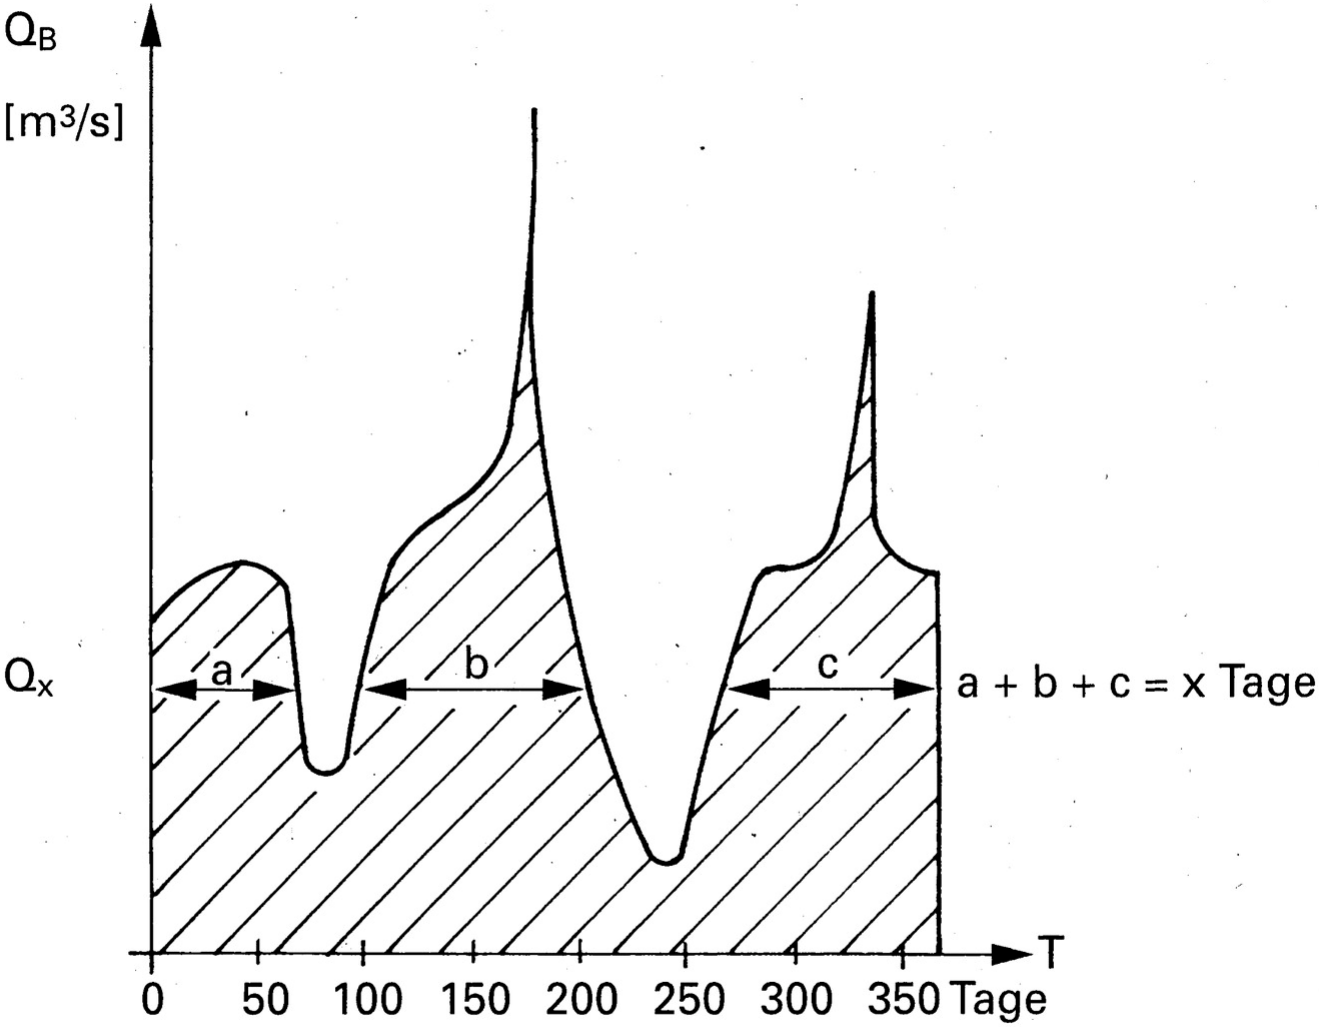
\includegraphics[width=0.95\textwidth, align=c]{images/Abflussganglinie.png}
    \end{center}
\end{minipage}

\vspace{0.25cm}



\subsection{Abflussdauerkurve}
Abfluss $Q_b$ in $\frac{m^3}{s}$ während eines Jahres (365 Tage), sortiert der Grösse nach\\
\begin{minipage}[c]{0.48\columnwidth}
    \begin{center}
        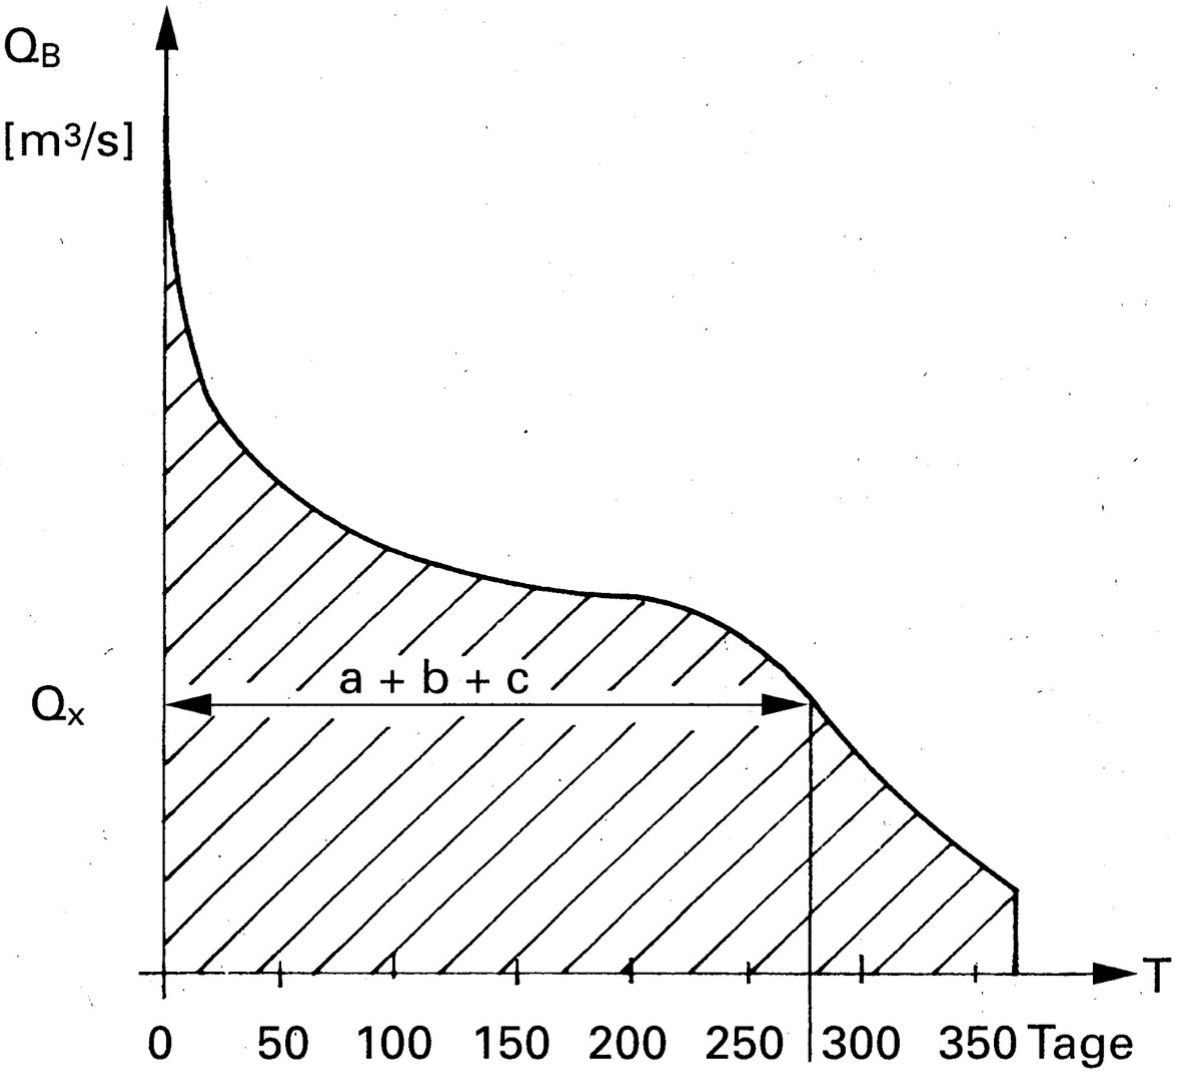
\includegraphics[width=0.95\textwidth, align=c]{images/Abflussdauerkurve.png}
    \end{center}
\end{minipage}

\vspace{0.25cm}

\textbf{Abfluss ist an 275 Tagen mindestens $Q_x$}



\subsection{Nutzwassermenge}
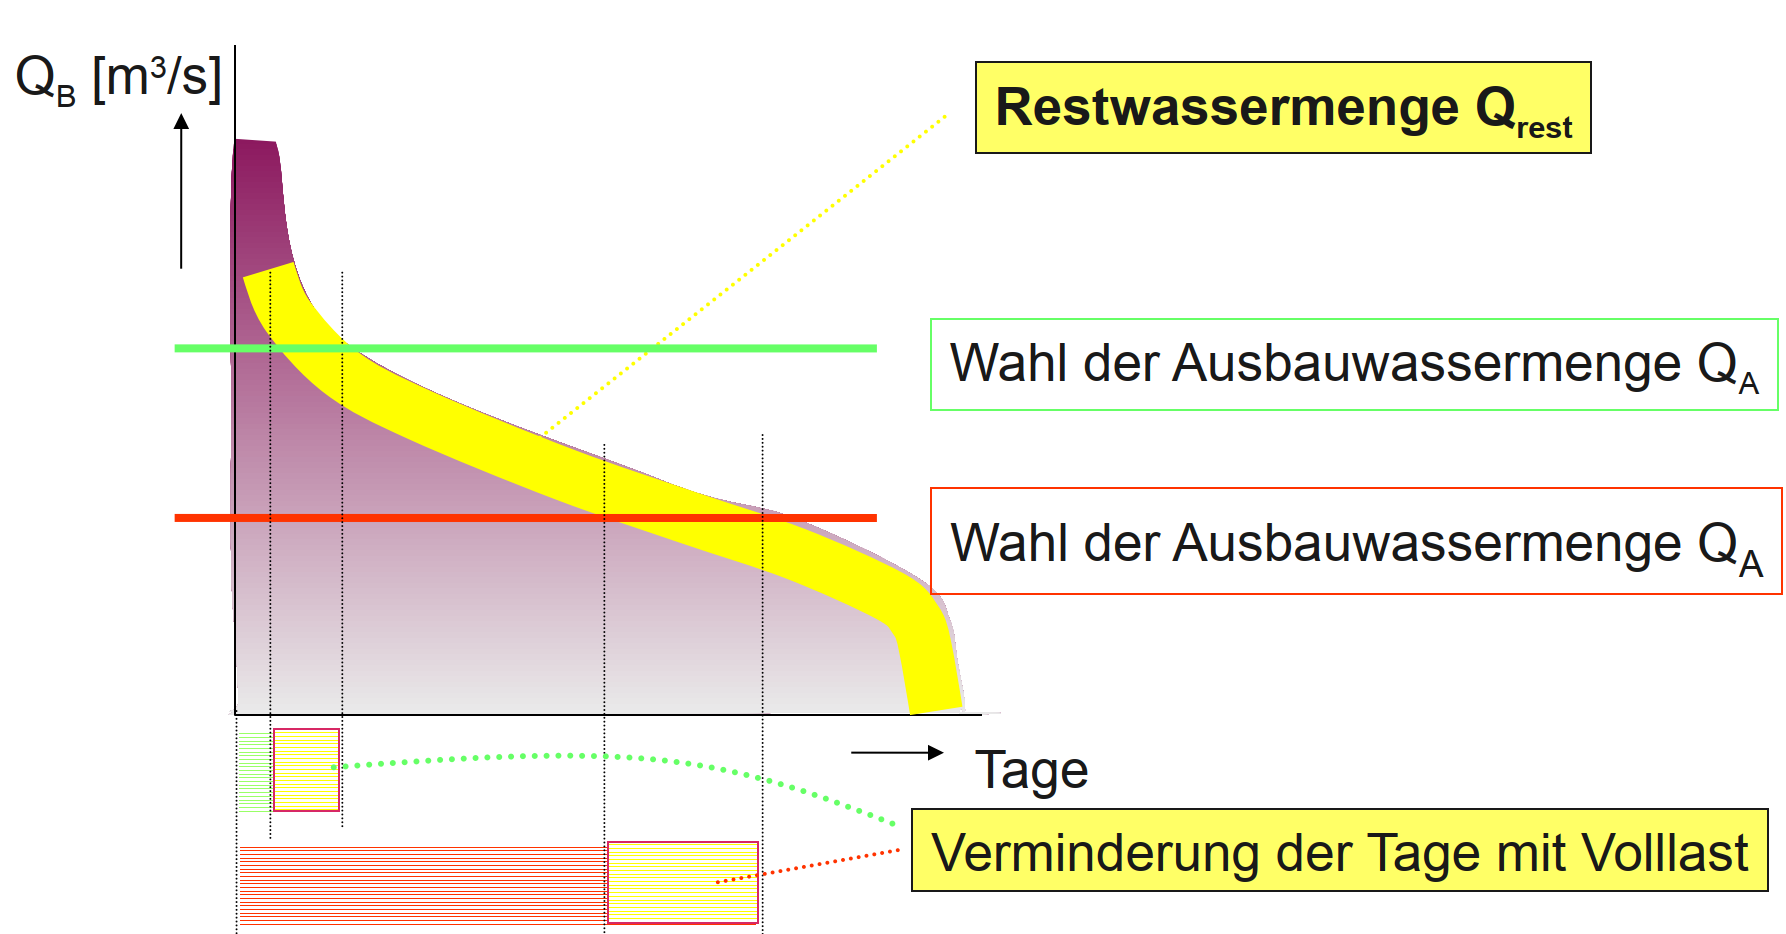
\includegraphics[width=0.95\columnwidth, align=c]{images/Nutzwassermenge.png}

\vspace{0.25cm}

$\boxed{Q_{Nutz} = Q_B - Q_{Rest}}$

\vspace{0.25cm}

\renewcommand{\arraystretch}{1.2} % Erhöht Zeilenhöhe für bessere Lesbarkeit
\begin{tabular}{@{} l p {6cm} l @{}}
    $[Q_{Nutz}]$    & Nutzwassermenge   \dotfill & $\frac{m^3}{s}$ \\
    $[Q_B]$         & Abflussmenge      \dotfill & $\frac{m^3}{s}$ \\
    $[Q_{Rest}]$    & Restwassermenge   \dotfill & $\frac{m^3}{s}$ \\
\end{tabular}
















        %\newpage
\section{Wasserkraft}


\subsection{Kontinuitätsgleichung des Durchflusses}
\begin{center}
    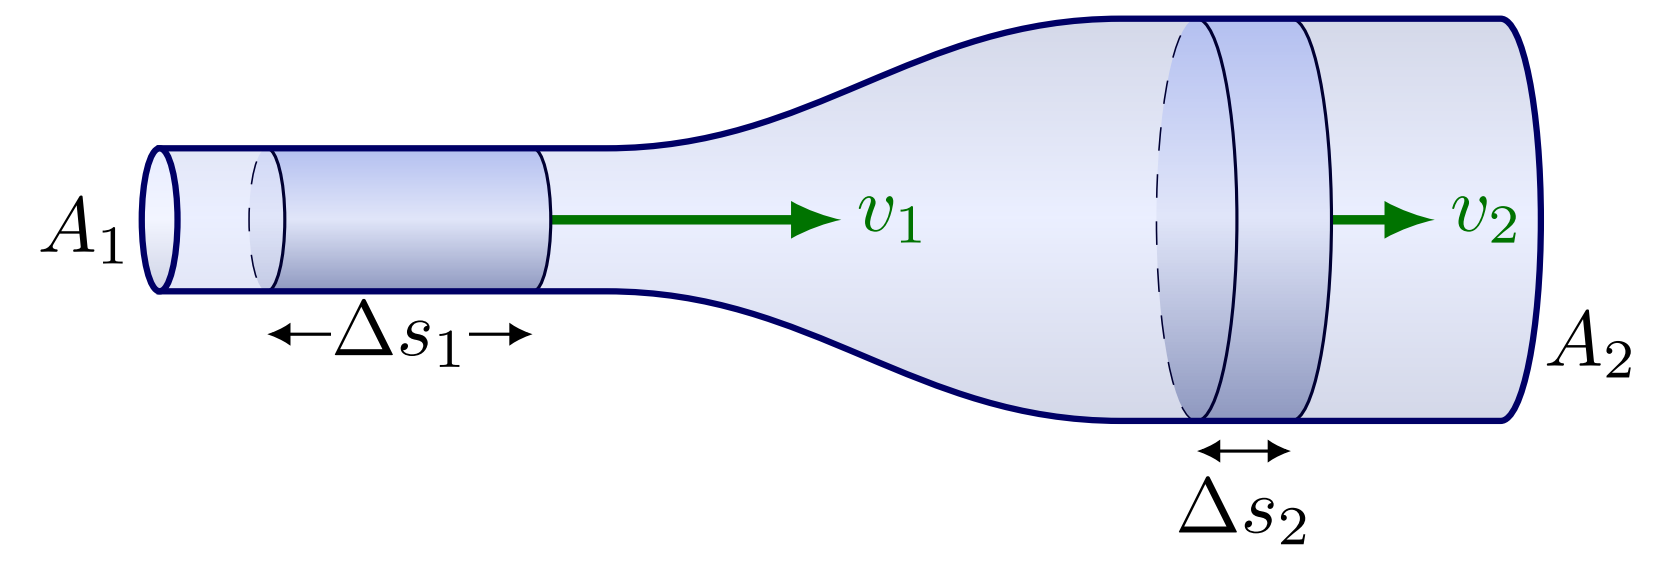
\includegraphics[width=0.9\columnwidth, align=c]{images/Kontinuitaet.png}
\end{center}

Die Kontinuitätsgleichung beschreibt die Erhaltung des Volumenstroms in einer strömenden Flüssigkeit:

\vspace{0.15cm}

$
\boxed{
    Q = A \cdot v 
} 
\quad
\boxed{
    Q_1 = Q_2 
} 
\quad
\boxed{
    A_1 \cdot v_1 = A_2 \cdot v_2
}
\quad
\boxed{
    Q = \dot{V} = \frac{\Delta V}{\Delta t} = \text{const} 
} 
$

\vspace{0.15cm}

\renewcommand{\arraystretch}{1.2} % Erhöht Zeilenhöhe für bessere Lesbarkeit
\begin{tabular}{@{} l p{6cm} l @{}}
    $[Q_x]$        & Durchflussrate                     \dotfill & $\mathrm{\frac{m^3}{s}}$ \\
    $[A_x]$        & Querschnittsfläche                 \dotfill & $\mathrm{m^2}$ \\
    $[v_x]$        & Fliessgeschwindigkeit              \dotfill & $\mathrm{\frac{m}{s}}$ \\
    $[\dot{V}]$    & Volumenstrom (Volumen pro Zeit)    \dotfill & $\mathrm{\frac{m^3}{s}}$ \\
    $[\Delta V]$   & Volumenänderung                    \dotfill & $\mathrm{m^3}$ \\
    $[\Delta t]$   & Zeitänderung                       \dotfill & $\mathrm{s}$ \\
\end{tabular}



\subsection{Bernoulli-Druck-Gleichung für Speicherwasserkraftwerke}

\begin{center}
    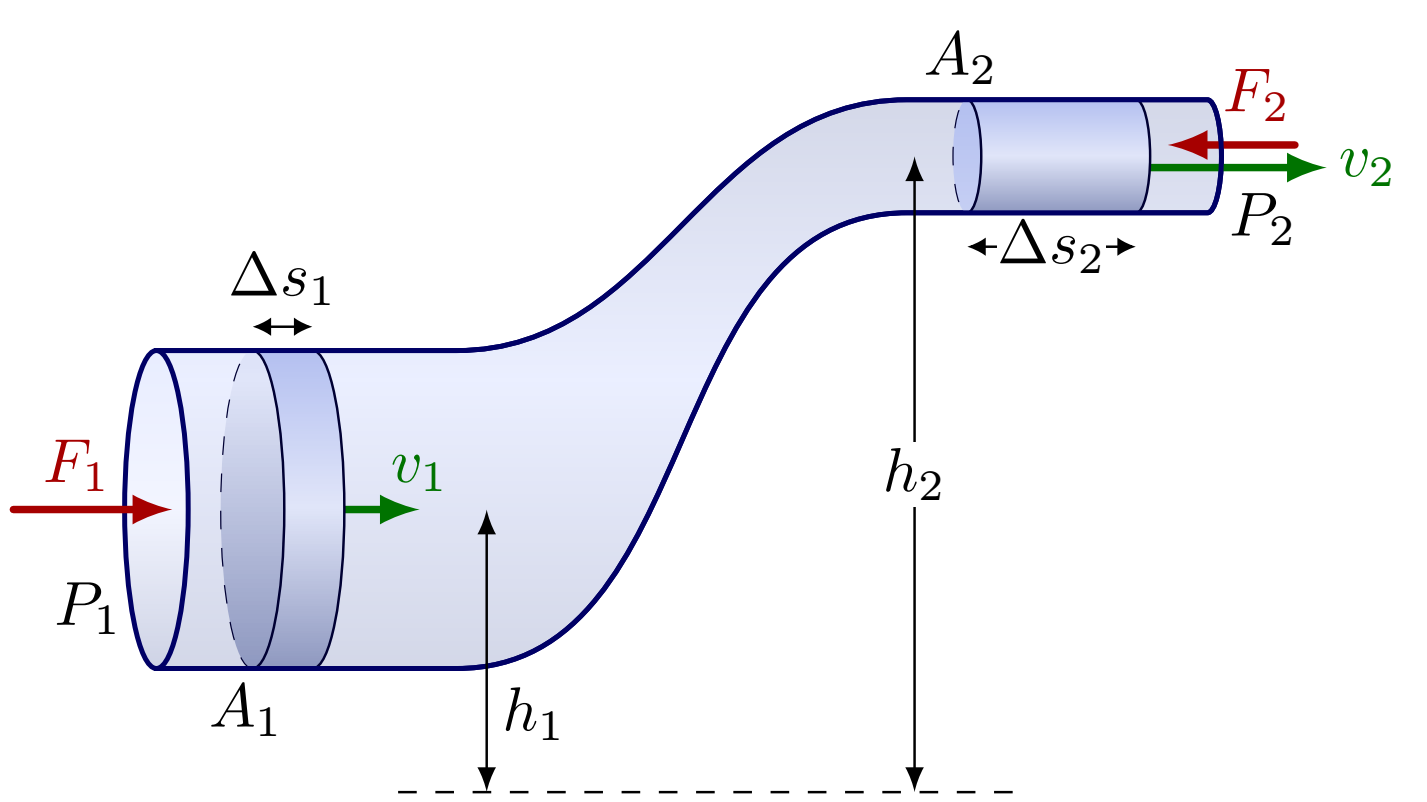
\includegraphics[width=0.9\columnwidth, align=c]{images/Bernoulli.png}
\end{center}

$\boxed{\frac{1}{2} \cdot \rho \cdot v^2 + \rho \cdot g \cdot z + p = \text{constant}}$

\vspace{0.15cm}

$
\boxed{
p_1 + \rho \cdot g \cdot h_1 + \frac{1}{2} \rho \cdot v_1^2 
= 
p_2 + \rho \cdot g \cdot h_2 + \frac{1}{2} \rho \cdot v_2^2
}
$

\vspace{0.15cm}

\renewcommand{\arraystretch}{1.2} % Erhöht Zeilenhöhe für bessere Lesbarkeit
\begin{tabular}{@{} l p {6cm} l @{}}
    $[\frac{1}{2} \rho v^2]$ & Kinetische Energie (je Kubikmeter) \dotfill & $\mathrm{\frac{J}{m^3}}$ \\
    $[\rho g z]$             & Potentielle Energie                 \dotfill & $\mathrm{\frac{J}{m^3}}$ \\
    $[p]$                    & Druckenergie                        \dotfill & $\mathrm{\frac{J}{m^3}}$ \\
\end{tabular}


\vspace{0.15cm}

$
\underbrace{p}_{A} + \underbrace{\rho g z}_{B} + \underbrace{\frac{1}{2}\rho v^2}_{C} = \underbrace{\text{constant}}_{D}
$


\subsection{Bernoulli-Höhen-Gleichung für Speicherwasserkraftwerke}

$\boxed{H = z + \frac{p}{\rho \cdot g} + \frac{v^2}{2 \cdot g} + \sum H_v}$

\vspace{0.15cm}

\renewcommand{\arraystretch}{1.3} % Erhöht Zeilenhöhe für bessere Lesbarkeit
\begin{tabular}{@{} l p {4cm} l @{}}
    $[H]$                           & Bruttogefälle                              \dotfill & $\mathrm{m}$ \\
    $[z]$                           & Höhenlage (potenzielle Energie)            \dotfill & $\mathrm{m}$ \\
    $[p]$                           & Druck                                      \dotfill & $\mathrm{Pa} = \mathrm{\frac{N}{m^2}}$ \\
    $[\rho]$                        & Dichte des Wassers                         \dotfill & $\mathrm{\frac{kg}{m^3}}$ \\
    $[g]$                           & Erdbeschleunigung                          \dotfill & $\mathrm{\frac{m}{s^2}}$ \\
    $[v]$                           & Geschwindigkeit                            \dotfill & $\mathrm{\frac{m}{s}}$ \\
    $\left[\frac{p}{\rho g}\right]$ & Druckhöhe                                  \dotfill & $\mathrm{m}$ \\
    $\left[\frac{v^2}{2g}\right]$   & Geschwindigkeitshöhe                       \dotfill & $\mathrm{m}$ \\
    $[\sum H_v]$                    & Hydraulische Energieverluste               \dotfill & $\mathrm{m}$ \\
\end{tabular}


\newcolumn
\subsection{Örtliche Energieverluste}

$\boxed{h_v = \zeta \cdot \frac{v^2}{2g}}$

\vspace{0.15cm}

\renewcommand{\arraystretch}{1.2} % Erhöht Zeilenhöhe für bessere Lesbarkeit
\begin{tabular}{@{} l p {4cm} l @{}}
    $[h_v]$     & Örtliche Energieverlusthöhe   \dotfill & $\mathrm{m}$ \\
    $[\zeta]$   & Verlustbeiwert (dimensionslos) \dotfill & $-$ \\
    $[v]$       & Geschwindigkeit               \dotfill & $\mathrm{\frac{m}{s}}$ \\
    $[g]$       & Erdbeschleunigung             \dotfill & $\mathrm{\frac{m}{s^2}}$ \\
\end{tabular}



\subsection{Reibungsverluste (Formel von Strickler)}

$\boxed{h_{\text{v,r}} = \frac{v^2 \cdot L}{K_{St}^2 \cdot R_h^{4/3}}}$

\vspace{0.15cm}

\renewcommand{\arraystretch}{1.2} % Erhöht Zeilenhöhe für bessere Lesbarkeit
\begin{tabular}{@{} l p {4cm} l @{}}
    $[h_{\text{v,r}}]$  & Reibungsverlusthöhe           \dotfill & $\mathrm{m}$ \\
    $[v]$               & Strömungsgeschwindigkeit      \dotfill & $\mathrm{\frac{m}{s}}$ \\
    $[L]$               & Länge der Strömungsstrecke    \dotfill & $\mathrm{m}$ \\
    $[K_{St}]$          & Rauhigkeitsbeiwert nach Strickler \dotfill & $\mathrm{\frac{m^{1/3}}{s}}$ \\
    $[R_h]$             & Hydraulischer Radius          \dotfill & $\mathrm{m}$ \\
\end{tabular}



\subsubsection{Tabelle Rauhigkeitsbeiwert $K_{St}$ nach Strickler}
\begin{tabular}{|l|l|c|}
    \hline
    \textbf{Material} & \textbf{Zustand} & \textbf{$K_{St}$ [m$^{1/3}$/s]} \\
    \hline
    Stahl & neu & 75 \\
    \hline
    Stahl & schlechter Zustand, verrostet, verkrustet & 60 \\
    \hline
    Beton & glatt & 85 \\
    \hline
    Beton & rauh & 60 \\
    \hline
    PE, PVC &  & 100 \\
    \hline
\end{tabular}


\subsubsection{Hydraulischer Radius}

\begin{minipage}[c]{0.48\columnwidth}
    \myul{\textbf{Rechteckqueerschnitt}}\\
    \begin{center}
        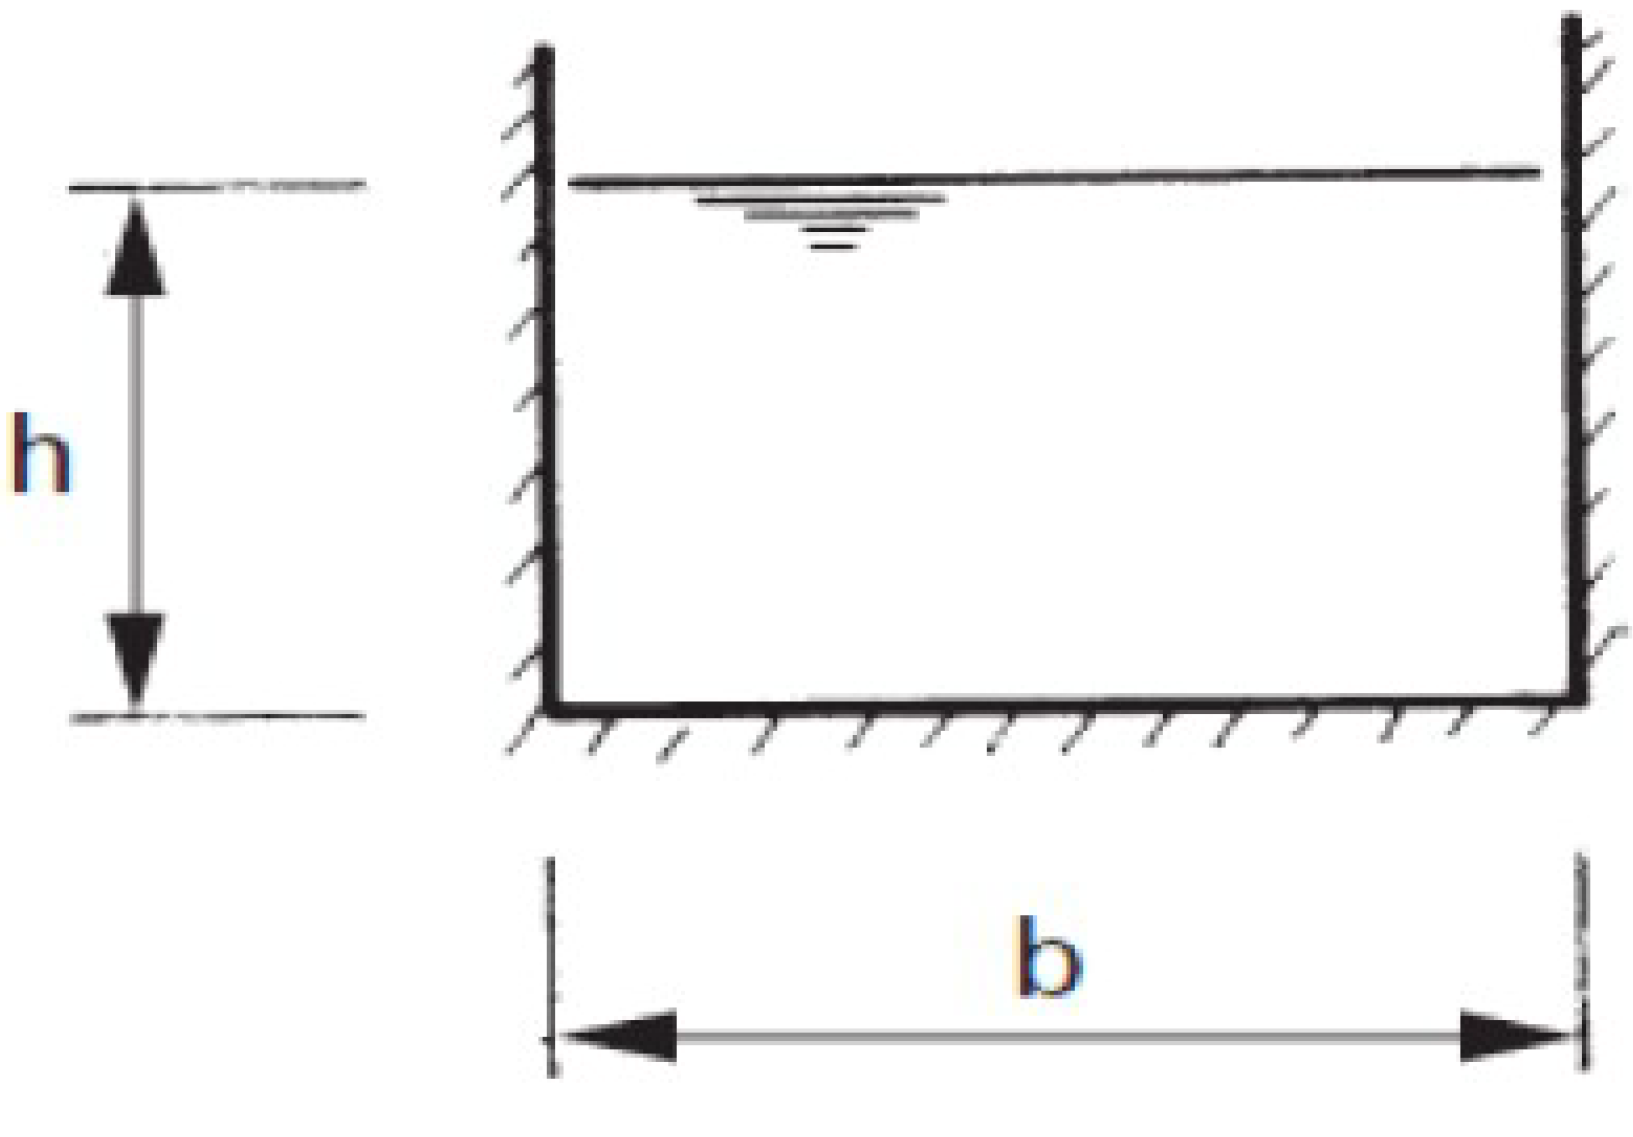
\includegraphics[width=0.9\textwidth, align=c]{images/Hydraulischer_Radius_Rechteck.png}
    \end{center}
\end{minipage}
\hfill
\vrule width 1pt % Vertikale Trennlinie mit 1pt Breite
\hfill
\begin{minipage}[c]{0.48\columnwidth}
    \myul{\textbf{Kreisqueerschnitt}}\\
    \begin{center}
        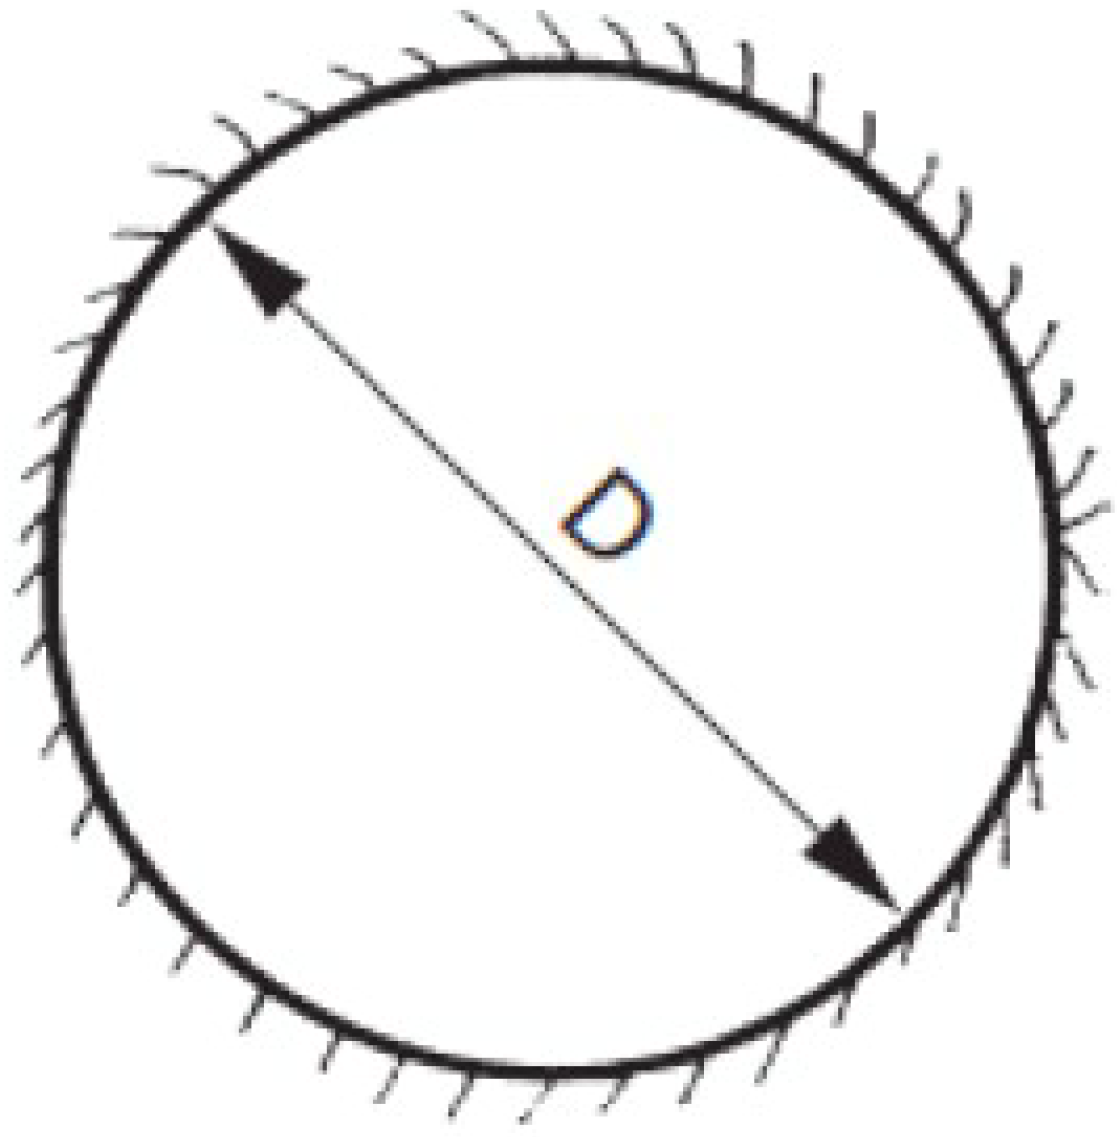
\includegraphics[width=0.65\textwidth, align=c]{images/Hydraulischer_Radius_Kreis.png}
    \end{center}
\end{minipage}

\vspace{0.25cm}

\begin{minipage}[c]{0.48\columnwidth}
    $\boxed{F = b \cdot h}$

    \vspace{0.15cm}

    $\boxed{P = b + 2 \cdot h}$

    \vspace{0.15cm}

    $\boxed{R_h = \frac{b \cdot h}{b + 2 \cdot h}}$ $\boxed{R_h = \frac{F}{P}}$
\end{minipage}
\hfill
\vrule width 1pt % Vertikale Trennlinie mit 1pt Breite
\hfill
\begin{minipage}[c]{0.48\columnwidth}
    $\boxed{F = \frac{D^2 \cdot \pi}{4}}$

    \vspace{0.15cm}

    $\boxed{P = D \cdot \pi}$

    \vspace{0.15cm}

    $\boxed{R_h = \frac{D}{4}}$ $\boxed{R_h = \frac{F}{P}}$
\end{minipage}

\vspace{0.15cm}

\renewcommand{\arraystretch}{1.2} % Erhöht Zeilenhöhe für bessere Lesbarkeit
\begin{tabular}{@{} l p {6cm} l @{}}
    $[F]$    & Abflussquerschnittsfläche         \dotfill & $\mathrm{m^2}$ \\
    $[P]$    & Benetzter Umfang                  \dotfill & $\mathrm{m}$ \\
    $[R_h]$  & Hydraulischer Radius              \dotfill & $\mathrm{m}$ \\
\end{tabular}





\subsection{Verlusthöhe durch Reibung}

$\boxed{h_{\text{v,r}} = \lambda \cdot \frac{L}{d_{\text{hy}}} \cdot \frac{v^2}{2 \cdot g} }
\quad
\boxed{h_{\text{v,r}} = \lambda \cdot \frac{L}{d_i} \cdot \frac{8 \cdot Q^2}{g \cdot \pi^2 \cdot d_i^4}}
\quad
\boxed{h_{\text{v,r}} = \frac{8 \cdot \lambda \cdot L \cdot Q^2}{g \cdot \pi^2 \cdot d_i^5}}$

\vspace{0.15cm}

\renewcommand{\arraystretch}{1.2} % Erhöht Zeilenhöhe für bessere Lesbarkeit
\begin{tabular}{@{} l p {6cm} l @{}}
    $[h_{\text{v,r}}]$  & Verlusthöhe durch Reibung      \dotfill & $\mathrm{m}$ \\
    $[L]$               & Länge                          \dotfill & $\mathrm{m}$ \\
    $[v_m]$             & Mittlere Geschwindigkeit       \dotfill & $\mathrm{\frac{m}{s}}$ \\
    $[Q]$               & Durchfluss                     \dotfill & $\mathrm{\frac{m^3}{s}}$ \\
    $[d_i]$             & Innendurchmesser               \dotfill & $\mathrm{m}$ \\
    $[d_{\text{hy}}]$   & Hydraulischer Durchmesser      \dotfill & $\mathrm{m}$ \\
    $[l_u]$             & Benetzter Umfang               \dotfill & $\mathrm{m}$ \\
    $[\lambda]$         & Verlustbeiwert                 \dotfill & $-$ \\
\end{tabular}


\vspace{0.15cm}

Zusammenhang des hydraulischen Durchmessers:

\vspace{0.15cm}

$
\boxed{d_{\text{hy}} = d_{\text{Kreisrohr}} = d_i = 4 \cdot R_{\text{hy}} = 4 \cdot \left(\frac{A}{l_u}\right)}
$


\newcolumn
\subsection{Reynolds-Zahl $\text{Re}$}

Die Reynolds-Zahl $\text{Re}$ beschreibt das Verhältnis von Trägheitskräften zu Zähigkeitskräften in einer Strömung und wird wie folgt berechnet:

\vspace{0.15cm}

$\boxed{\text{Re} = \frac{v_m \cdot d_{\text{hy}}}{\nu}}$ \quad Bemerkung: $d_{\text{hy}} = d_{\text{Kreisrohr}} = d_i$

\vspace{0.15cm}

\renewcommand{\arraystretch}{1.2} % Erhöht Zeilenhöhe für bessere Lesbarkeit
\begin{tabular}{@{} l p {6cm} l @{}}
    $[\text{Re}]$     & Reynolds-Zahl (dimensionslos)                        \dotfill & $-$ \\
    $[v_m]$           & Mittlere Strömungsgeschwindigkeit                    \dotfill & $\mathrm{\frac{m}{s}}$ \\
    $[d_{\text{hy}}]$ & Hydraulischer Durchmesser                            \dotfill & $\mathrm{m}$ \\
    $[d_i]$           & Innendurchmesser (für Kreisrohr gleich $d_{\text{hy}}$) \dotfill & $\mathrm{m}$ \\
    $[\nu]$           & Kinematische Viskosität                              \dotfill & $\mathrm{\frac{m^2}{s}}$ \\
\end{tabular}




\subsection{Verlustbeiwert }

$
\boxed{
\lambda = \left(\frac{1}{-2 \cdot \log \left( \frac{\varepsilon}{3{,}71} \right)}\right)^2
}
\quad
\boxed{
\lambda = \left(\frac{1}{-2 \cdot \log \left( \frac{k}{d_{hy} \cdot 3{,}71} \right)}\right)^2
}
$

\vspace{0.15cm}

\renewcommand{\arraystretch}{1.2}
\begin{tabular}{@{} l p{6cm} l @{}}
    $[\lambda]$ & Verlustbeiwert \dotfill & $-$ \\
    $[k]$ & äquivalente Rauheit \dotfill & mm \\
    $[d_{\text{hy}}]$ & Hydraulischer Durchmesser \dotfill & m \\
\end{tabular}



\subsection{Nettogefälle $H_n$}
$
\boxed{
H_n = H - \sum H_v - \frac{v^2}{2g}
}
\quad
\boxed{\sum H_v = C \cdot Q^2}
$

\vspace{0.15cm}

\renewcommand{\arraystretch}{1.2}
\begin{tabular}{@{} l p{6cm} l @{}}
    $[H_n]$       & Nettofallhöhe \dotfill & m \\
    $[H]$         & Bruttogefälle \dotfill & m \\
    $\left[\sum H_v\right]$ & Summe der hydraulischen Verluste \dotfill & m \\
    $[C]$         & Faktor bei Bestimmung der Verluste \dotfill & $\frac{\text{s}^{2}}{\text{m}^5}$ \\
    $[Q]$         & Volumenstrom \dotfill & $\frac{\text{m}^3}{\text{s}}$ \\
    $[v]$         & Strömungsgeschwindigkeit im Unterwasser \dotfill & $\frac{\text{m}}{\text{s}}$ \\
    $[g]$         & Erdbeschleunigung $g = 9{,}81$ \dotfill & $\frac{\text{m}}{\text{s}^2}$ \\
\end{tabular}



\subsection{Hydraulische Leistung $P_{\text{hyd}}$}

$
\boxed{P_{\text{hyd}} = \frac{m \cdot g \cdot H_n}{t} }
\quad
\boxed{P_{\text{hyd}} = \rho \cdot Q \cdot g \cdot H_n}
\quad
\boxed{\frac{\text{m}}{\text{t}} = \rho \cdot Q}
$

\vspace{0.15cm}

\renewcommand{\arraystretch}{1.2}
\begin{tabular}{@{} l p{6cm} l @{}}
    $[P_{\text{hyd}}]$  & Hydraulische Leistung \dotfill                & $\text{W}$ \\
    $[m]$               & Masse \dotfill                                & $\text{kg}$ \\
    $[g]$               & Erdbeschleunigung, $g = 9{,}81$ \dotfill      & $\frac{\text{m}}{\text{s}^2}$ \\
    $[H_n]$             & Nettofallhöhe \dotfill                        & $\text{m}$ \\
    $[t]$               & Zeit \dotfill                                & $\text{s}$ \\
    $[\rho]$            & Dichte des Wassers, $\rho = 1000$ \dotfill    & $\frac{\text{kg}}{\text{m}^3}$ \\
    $[Q]$               & Nutzwassermenge \dotfill                      & $\frac{\text{m}^3}{\text{s}}$\\ 
\end{tabular}



\subsection{Mechanische Leistung $P_{\text{mech}}$}

$
\boxed{P_{\text{mech}} = \eta_t \cdot P_{\text{hyd}}} 
\quad 
\boxed{P_{\text{mech}} = \eta_t \cdot \rho \cdot Q \cdot g \cdot H_n}
$

\vspace{0.15cm}

\renewcommand{\arraystretch}{1.2}
\begin{tabular}{@{} l p{7cm} l @{}}
    $[P_{\text{mech}}]$  & Mechanische Leistung an der Turbinen-Generator-Welle \dotfill & $\text{W}$ \\
    $[P_{\text{hyd}}]$   & Hydraulische Leistung \dotfill                               & $\text{W}$ \\
    $[\eta_t]$           & Turbinenwirkungsgrad \dotfill                               & $-$ \\
\end{tabular}



\subsection{Elektrische Leistung $P_{\text{el}}$}

$
\boxed{P_{\text{el}} = \eta_g \cdot P_{\text{mech}}} 
\quad 
\boxed{P_{\text{el}} = \eta_g \cdot \eta_t \cdot \rho \cdot Q \cdot g \cdot H_n}
$

\vspace{0.15cm}

\renewcommand{\arraystretch}{1.2}
\begin{tabular}{@{} l p{6cm} l @{}}
    $[P_{\text{el}}]$     & Elektrische Leistung an den Generatorklemmen \dotfill & $\text{W}$ \\
    $[P_{\text{mech}}]$   & Mechanische Leistung \dotfill                          & $\text{W}$ \\
    $[\eta_g]$            & Generatorwirkungsgrad \dotfill                         & $-$ \\
\end{tabular}



\subsection{Elektrische Energie $E$}

$
\boxed{E = \int P_{\text{el}} \cdot dt}
\quad
\boxed{E = \int \eta_g \cdot \eta_t \cdot Q \cdot H_n \cdot \rho \cdot g \cdot dt}
\quad
\boxed{E = \rho \cdot g \cdot \int \eta_g \cdot \eta_t \cdot Q \cdot H_n \cdot dt}
$

\vspace{0.15cm}

\renewcommand{\arraystretch}{1.2}
\begin{tabular}{@{} l p{6cm} l @{}}
    $[E]$               & Elektrische Energie \dotfill                           & $\text{Ws}$ \\
    $[P_{\text{el}}]$   & Elektrische Leistung \dotfill                          & $\text{W}$ \\
    $[\eta_g]$          & Generatorwirkungsgrad \dotfill                         & $-$ \\
    $[\eta_t]$          & Turbinenwirkungsgrad \dotfill                          & $-$ \\
    $[Q]$               & Nutzwassermenge \dotfill                               & $\frac{\text{m}^3}{\text{s}}$ \\
    $[H_n]$             & Nettofallhöhe \dotfill                                 & $\text{m}$ \\
    $[\rho]$            & Dichte des Wassers, $\rho = 1000$ \dotfill             & $\frac{\text{kg}}{\text{m}^3}$ \\
    $[g]$               & Erdbeschleunigung, $g = 9{,}81$ \dotfill               & $\frac{\text{m}}{\text{s}^2}$ \\
    $[t]$               & Zeit \dotfill                                           & $\text{s}$ \\
\end{tabular}

























































        %\section{Talsperren}


\subsection{Bogenstaumauer}

\begin{minipage}[c]{0.38\columnwidth}
    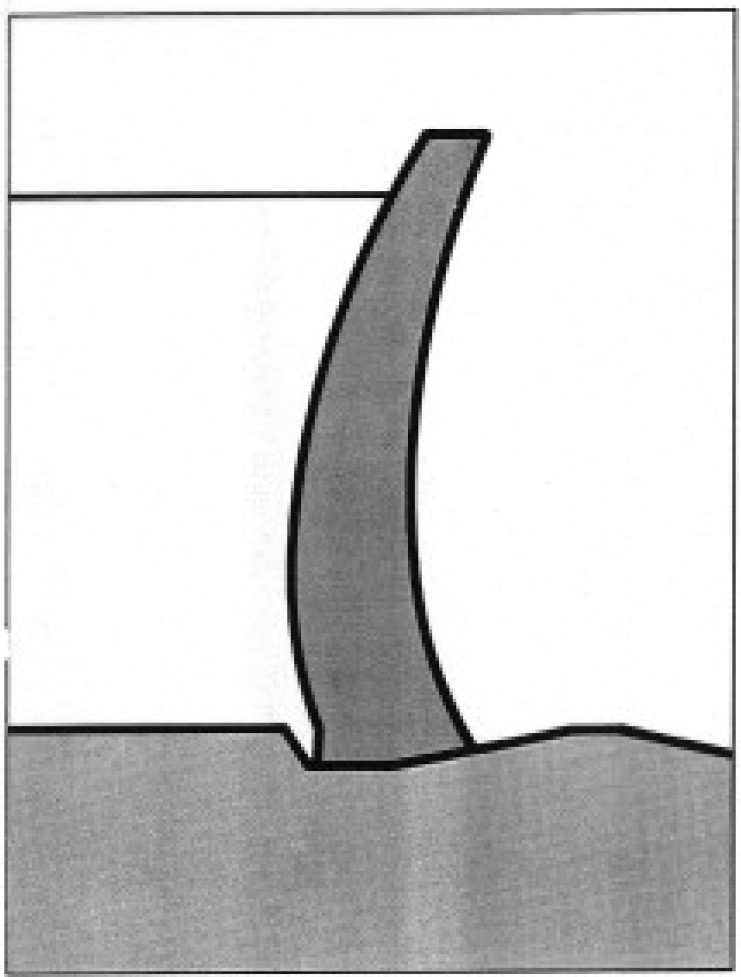
\includegraphics[width=0.98\columnwidth, align=c]{images/Talsperre_1.jpg}
\end{minipage}
\hfill
\begin{minipage}[t]{0.58\columnwidth}
    \begin{itemize}
    \item Beton
    \item Schlank
    \item Kraft wird links und rechts in den Hang geleitet (Gewölbewirkung)
    \item Beispiel: Verzasca Damm (Tessin)
    \end{itemize}
\end{minipage}



\subsection{Gewichtsstaumauer}
\begin{minipage}[c]{0.38\columnwidth}
    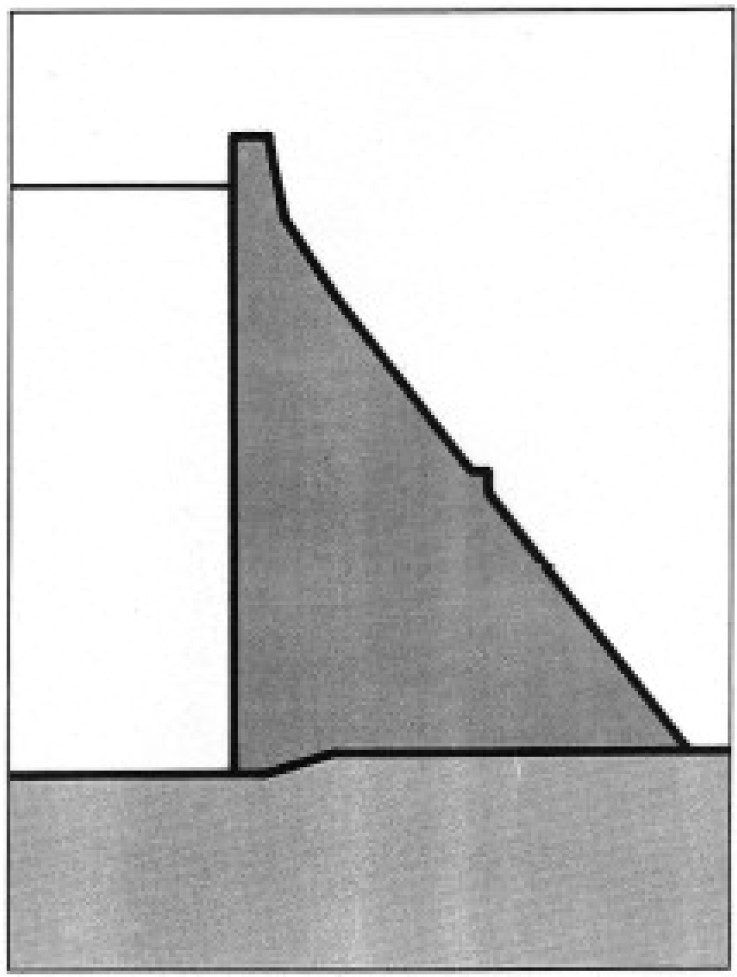
\includegraphics[width=0.98\columnwidth, align=c]{images/Talsperre_2.jpg}
\end{minipage}
\hfill
\begin{minipage}[c]{0.58\columnwidth}
    \begin{itemize}
  \item Beton oder Mauerwerk
  \item Hohes Eigengewicht
  \item Kraft wird durch Eigengewicht gehalten
  \item Beispiel: Grande Dixence (Wallis) Höchste Gewichtsstaumauer der Welt
\end{itemize}

\end{minipage}

\subsection{Staudamm}


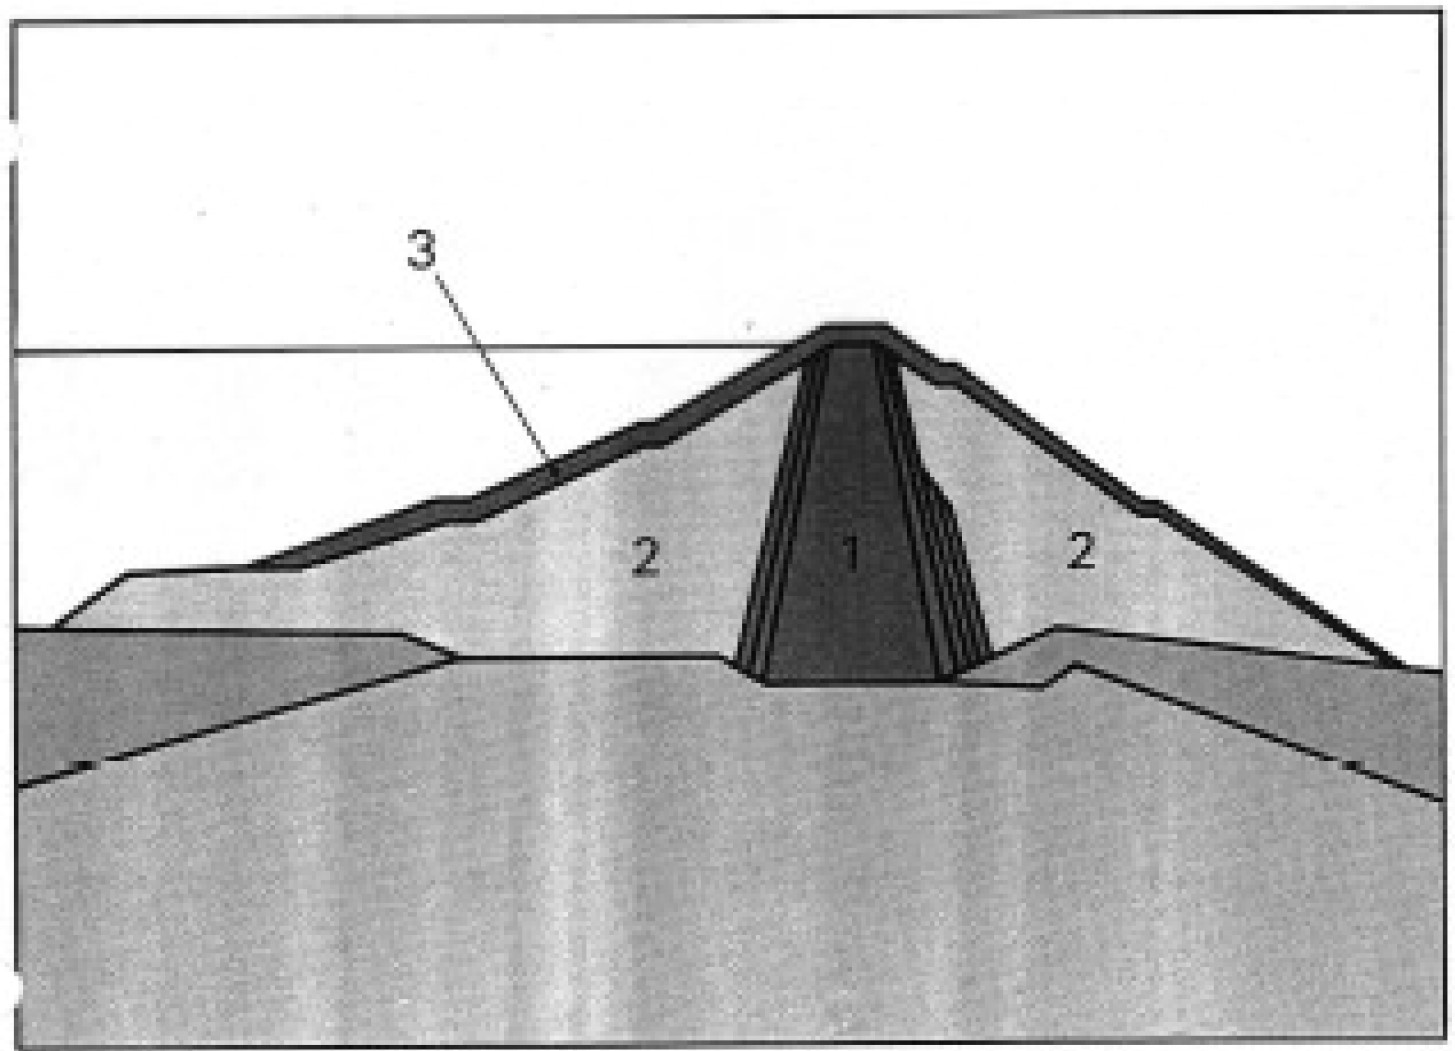
\includegraphics[width=0.8\columnwidth, align=c]{images/Talsperre_3.jpg}

\vspace{0.15cm}

\begin{enumerate}
    \item Kern 
    \item Stützkörper
    \item Schutzschicht
\end{enumerate}

\vspace{0.15cm}

\begin{itemize}
  \item Aufgeschüttet
  \item Flacher Böschungswinkel
  \item Steinschüttung unterschiedlicher Korngrösse
  \item Beispiel: Stausee Mattmark (Wallis) (Höchster Erdschüttdamm der Welt)
\end{itemize}

\vspace{0.15cm}


\subsection{}


\subsection{}


\subsection{}


\subsection{}


\subsection{}


\subsection{}


\subsection{}
        %\newpage
\section{Abschlussorgane bei Speicherkraftwerken}

\subsection{Schützen}
\textbf{Aufgabe:}  
Binäre Regelung des Wasserdurchflusses („Auf und zu“)

\textbf{Anwendung:}  
Grundablass, Seeabschluss, Abschluss gegen das Unterwasser

\textbf{\textcolor{green}{Vorteile:}}  
Einfacher Aufbau, sichere Absperrung

\textbf{\textcolor{red}{Nachteile:}}  
Keine Zwischenstellungen („halb offen“ nicht möglich)

\textbf{Beispiel:}  
Regulierschütz und Reserveschütz beim Grundablass

\textbf{Sonstiges:}  
Zwei Schützen pro Grundablass für Betrieb und Revision; schnelle Schliess- und Öffnungszeiten sind entscheidend, um Druckstösse zu vermeiden.

\subsection{Klappen}
\textbf{Aufgabe:}  
Wasserfluss absperren (Notverschluss, Wartung)

\textbf{Anwendung:}  
Saugrohrklappen beim Kraftwerk Mapragg

\textbf{\textcolor{green}{Vorteile:}}  
Schnelles Schliessen, einfacher Aufbau

\textbf{\textcolor{red}{Nachteile:}}  
Keine Regelungsfunktion („halb offen“ nicht möglich)

\textbf{Beispiel:}  
Saugrohrklappen Mapragg

\textbf{Sonstiges:}  
Dienen als definitiver Abschluss bei Stillstand oder Wartung; Schliess- und Öffnungszeiten dürfen nicht verändert werden, um Druckstösse zu vermeiden.

\subsection{Drosselklappen}
\textbf{Aufgabe:}  
Regelbarer Durchfluss durch horizontales Verschieben (Spalt lässt Wasser durch)

\textbf{Anwendung:}  
Einsatz bei variablen Durchflüssen

\textbf{\textcolor{green}{Vorteile:}}  
Regelbarkeit des Durchflusses möglich

\textbf{\textcolor{red}{Nachteile:}}  
Höhere hydraulische Verluste

\textbf{Beispiel:}  
Horizontal verschiebbarer Rohrschieber

\textbf{Sonstiges:}  
Wird nur selten bei Speicher- oder Laufwasserkraftwerken eingesetzt, da dort meist binäre Regelung bevorzugt wird.

\subsection{Kugelschieber}
\textbf{Aufbau:}  
Drehbare Kugel mit Loch

\textbf{Aufgabe:}  
Absperren des Wasserflusses mit nahezu verlustfreiem Durchfluss im offenen Zustand

\textbf{Anwendung:}  
Definitiver Abschluss (Betriebsring und Reservering)

\textbf{\textcolor{green}{Vorteile:}}  
Im offenen Zustand nahezu verlustfrei

\textbf{\textcolor{red}{Nachteile:}}  
Wartung und Betrieb der Dichtung (Betriebsring) aufwändig

\textbf{Beispiel:}  
Kugelschieber in Wasserkraftwerken mit Betriebsring und Reservering

\textbf{Sonstiges:}  
Betriebsring sorgt für Abdichtung zwischen Gehäuse und Kugel, Reservering wird nur bei Revision geschlossen und gegen Wiederöffnen gesichert.

\subsection{Ring- und Eckringschieber}
\textbf{Aufgabe:}  
Steuerung des Wasserflusses innerhalb oder ausserhalb des Rohres

\textbf{Anwendung:}  
Ringschieber: innerhalb des Rohres; Eckringschieber: ausserhalb des Rohres

\textbf{\textcolor{green}{Vorteile:}}  
Flexibler Einbau, verschiedene Steuerungsmöglichkeiten

\textbf{\textcolor{red}{Nachteile:}}  
Erhöhter Konstruktions- und Wartungsaufwand

\textbf{Beispiel:}  
Ringschieber und Eckringschieber bei variablen Wasserführungen

\textbf{Sonstiges:}  
Ermöglichen Zwischenstellungen (feine Regelung), können jedoch zu höheren hydraulischen Verlusten führen.


        %\section{Stauanlagen bei Laufwasserkraftwerken}


\subsubsection{Unterschied zu Speicherkraftwerken}
Das Wasser muss immer fliessen können – es kann weder gestoppt noch umgeleitet werden.

\subsubsection{Abfluss}
Muss auch während Instandhaltungsarbeiten gewährleistet sein. Eine mindestens (n-1) -Sicherheit muss für wehrabschlüsse vorhanden sein.
Auch beim Ausfall eines Ablassorgans (Verstopfung) muss das definierte Hächsthochwasser beherrschbar sein.

\subsection{Ausleitungskraftwerke (Umleitungskraftwerke)}

\vspace{0.15cm}

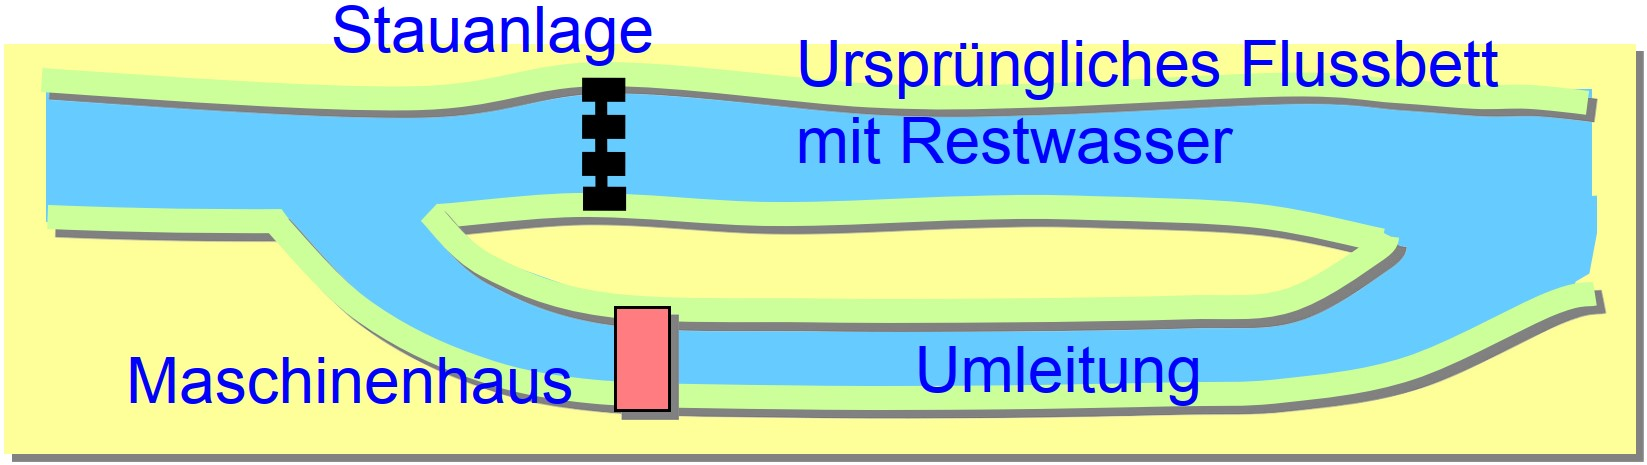
\includegraphics[width=0.98\columnwidth, align=c]{images/Ausleitungskraftwerke.jpg}
\begin{itemize}
  \item Bessere Ausnutzung des Gefälles in flachen Tälern
  \item Wasserwirtschaftliche Belange
  \item Aspekte hinsichtlich des Grundwassers sowie kulturtechnische Erwägungen
  \item Einfacher zum Bauen
\end{itemize}



\subsection{Flusskraftwerke}

\textbf{Bauweise 1}\\
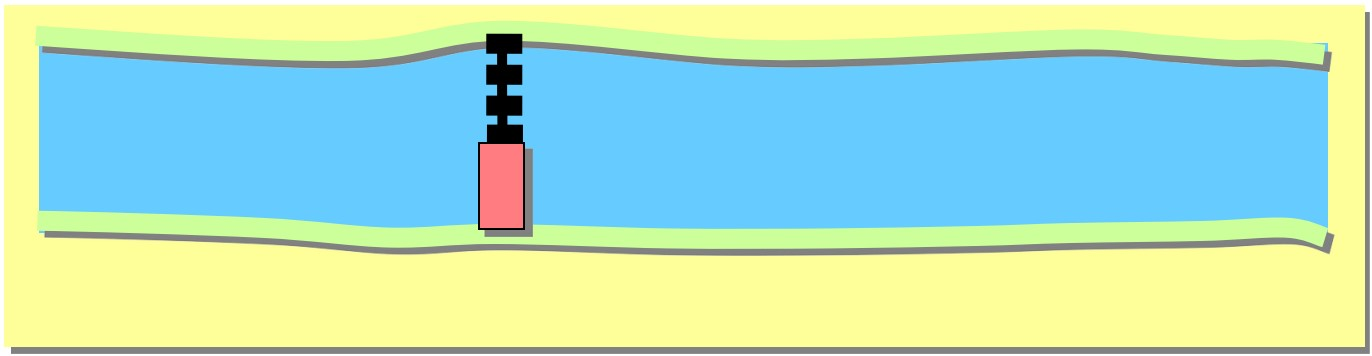
\includegraphics[width=0.98\columnwidth, align=c]{images/Flusskraftwerke_Bauweise_1.jpg}
\vspace{0.15cm}
\textbf{Bauweise 2}\\
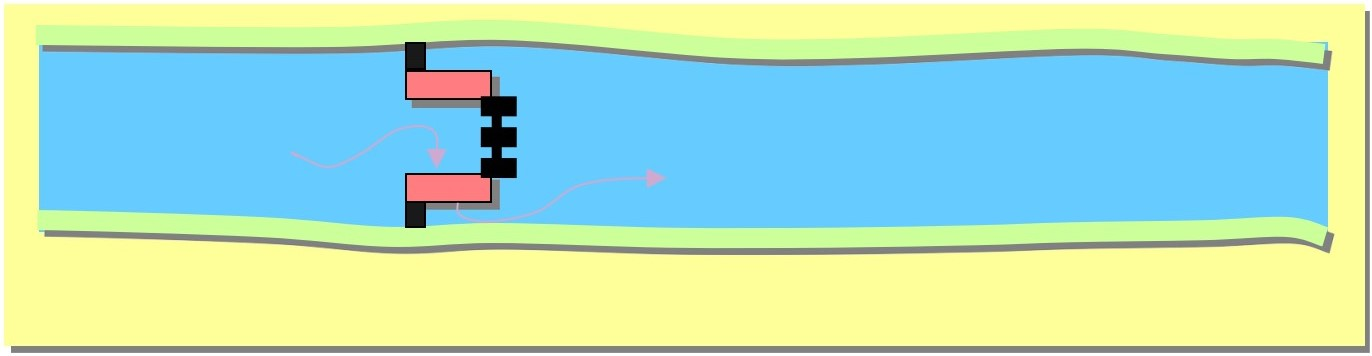
\includegraphics[width=0.98\columnwidth, align=c]{images/Flusskraftwerke_Bauweise_2.jpg}
\vspace{0.15cm}
\textbf{Bauweise 3}\\
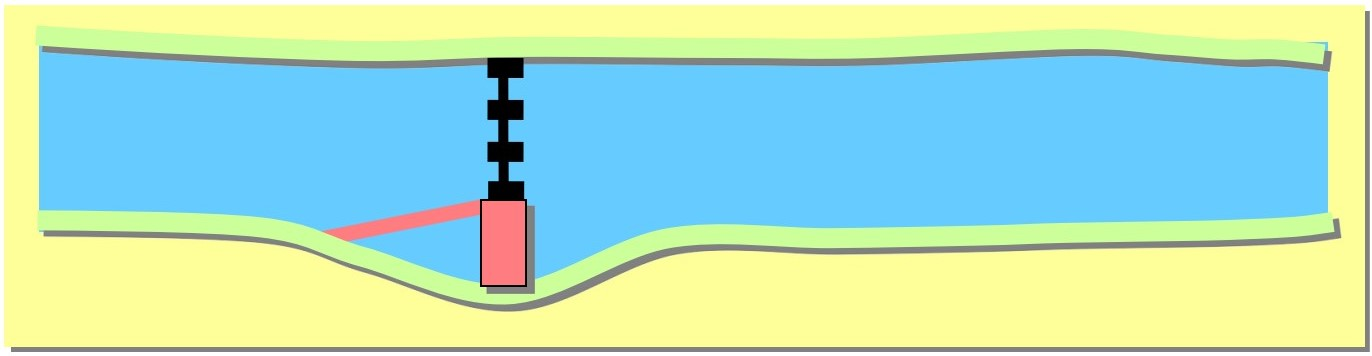
\includegraphics[width=0.98\columnwidth, align=c]{images/Flusskraftwerke_Bauweise_3.jpg}
\vspace{0.15cm}

Moderne Flusskraftwerke werden heute gemäss Bauweise 1 gebaut.

Der Wirkungsgrad bei Bauweise 2 und 3 ist schlechter als bei Bauweise 1.


\subsection{Arten von Wehr- und Sektorverschlüssen}
\includegraphics[width=0.98\columnwidth, align=c]{images/Arten_Wehr_und_Sektorverschlüsse_1.png}

\includegraphics[width=0.98\columnwidth]{images/Arten_Wehr_und_Sektorverschlüsse_2.png}



\subsection{Ort des Maschinenhauses}
Maschinenhaus auf der Kurvenaussenseite

\textbf{\textcolor{green}{Vorteile:}}  
\begin{itemize}
    \item Druckhöhe vor den Trubinen ist grösser
\end{itemize}

\textbf{\textcolor{red}{Nachteile:}}  

\begin{itemize}
    \item Geschwemsel lagert sich vor allem vor dem Rechen ab
    \item Bei starkem Geschwemseltrieb muss eventuell sogar das Kraftwerk abgestellt werden
\end{itemize}


        %\newpage
\section{Wasserkraftwerk-Typen}

\subsection{Klassifizierung}

\begin{itemize}
    \item Laufwasserkraftwerke
    \item Mitteldruckanlagen
    \item Hochdruck- (Speicher-) Anlagen
    \item Pumpspeicherkraftwerke
    \item Gezeitenkraftwerke
    \item Wellenkraftwerke
    \item Wasserwirbelkraftwerke
\end{itemize}


\subsection{Einteilung nach technischen Aspekten}
\begin{itemize}
    \item \textbf{Laufwasserkraftwerke}
    \begin{itemize}
        \item Flusskraftwerke
        \begin{itemize}
            \item Blockbauweise
            \item Buchtenkraftwerke
            \item Zwillingsbauweise (beidseitige Anordnung)
            \item \dots
        \end{itemize}
        \item Ausleitungskraftwerke
    \end{itemize}
    
    \item \textbf{Speicherkraftwerke} mit natürlichem Zufluss
    \item \textbf{Pumpspeicherkraftwerke} (Speicherkraftwerke mit oder ohne natürlichem Zufluss)
    \item Gezeitenkraftwerke
    \item Wellenkraftwerke
\end{itemize}



\subsection{Einteilung nach energiewirtschaftlichen Aspekten}
\begin{itemize}
    \item Grundlastkraftwerke (häufig verwendet, Laufwasser, Speicher mit vielen Volllaststunden)
    \item Mittellastkraftwerke
    \item Spitzenlastkraftwerke (Speicher mit wenig Volllaststunden)
\end{itemize}



\subsection{Einteilung nach Betriebsart}
\begin{itemize}
    \item Verbundbetrieb (im Normalbetrieb alle Kraftwerke in der Schweiz)
    \item Inselbetrieb (Unabhängig vom Netz)
\end{itemize}



\subsection{Einteilung nach der installierten Leistung}
\begin{itemize}
    \item Kleinwasserkraftwerke (in der Regel kleiner 10 MW)
    \item Grosswasserkraftwerke (P > 10 MW)
\end{itemize}



\subsection{Einteilung nach wasserwirtschaftlichen Aspekten}
\begin{itemize}
    \item Wasserkraftwerke, die ausschliesslich elektrische Energie produzieren
    \item Wasserkraftanlagen für mehrere wasserwirtschaftliche Zielsetzungen (Mehrzweckanlagen, z.\,B. Trinkwasser)
\end{itemize}



\subsection{Wasserturbinen und Pumpen}

\begin{itemize}
    \item \textbf{Aktionsturbinen:} Arbeit aus kinetischer Energie-Differenz
    \begin{itemize}
        \item \textbf{Peltonturbinen}
    \end{itemize}

\item \textbf{Reaktionsturbinen:} Arbeit aus Druckdifferenz vor und nach Turbine
    \begin{itemize}
        \item \textbf{Francisturbinen} (spiralförmig)
        \item \textbf{Kaplanturbinen} (propellerförmig)
        \item Rohrturbinen
        \item Kreiselpumpen als Turbinen
    \end{itemize}
\end{itemize}



\subsection{Laufwasserkraftwerke LWK}

\begin{center}
    \includegraphics[width=0.95\columnwidth, align=c]{images/Laufwasserkraftwerke.png}
\end{center}

\begin{minipage}[c]{0.38\columnwidth}
    \begin{tabular}{c l}
        1 & Oberwasser \\ 
        2 & Unterwasser \\ 
        3 & Maschinenhaus \\
        4 & Stauwehr \\
        5 & Transformatoren \\
    \end{tabular}
\end{minipage}
\hfill
\begin{minipage}[c]{0.58\columnwidth}
    \begin{tabular}{c l}
        6 & Schaltanlage \\
        7 & Leitungen \\
        8 & Betriebsgebäude \\
        9 & Fischtreppe \\
        10 & Einrichtung für den Schiffstransport \\
    \end{tabular}
\end{minipage}



\subsection{LWK mit Kaplanturbinen}

\begin{itemize}
    \item Turbine Vertikal verbaut
\end{itemize}

\begin{center}
    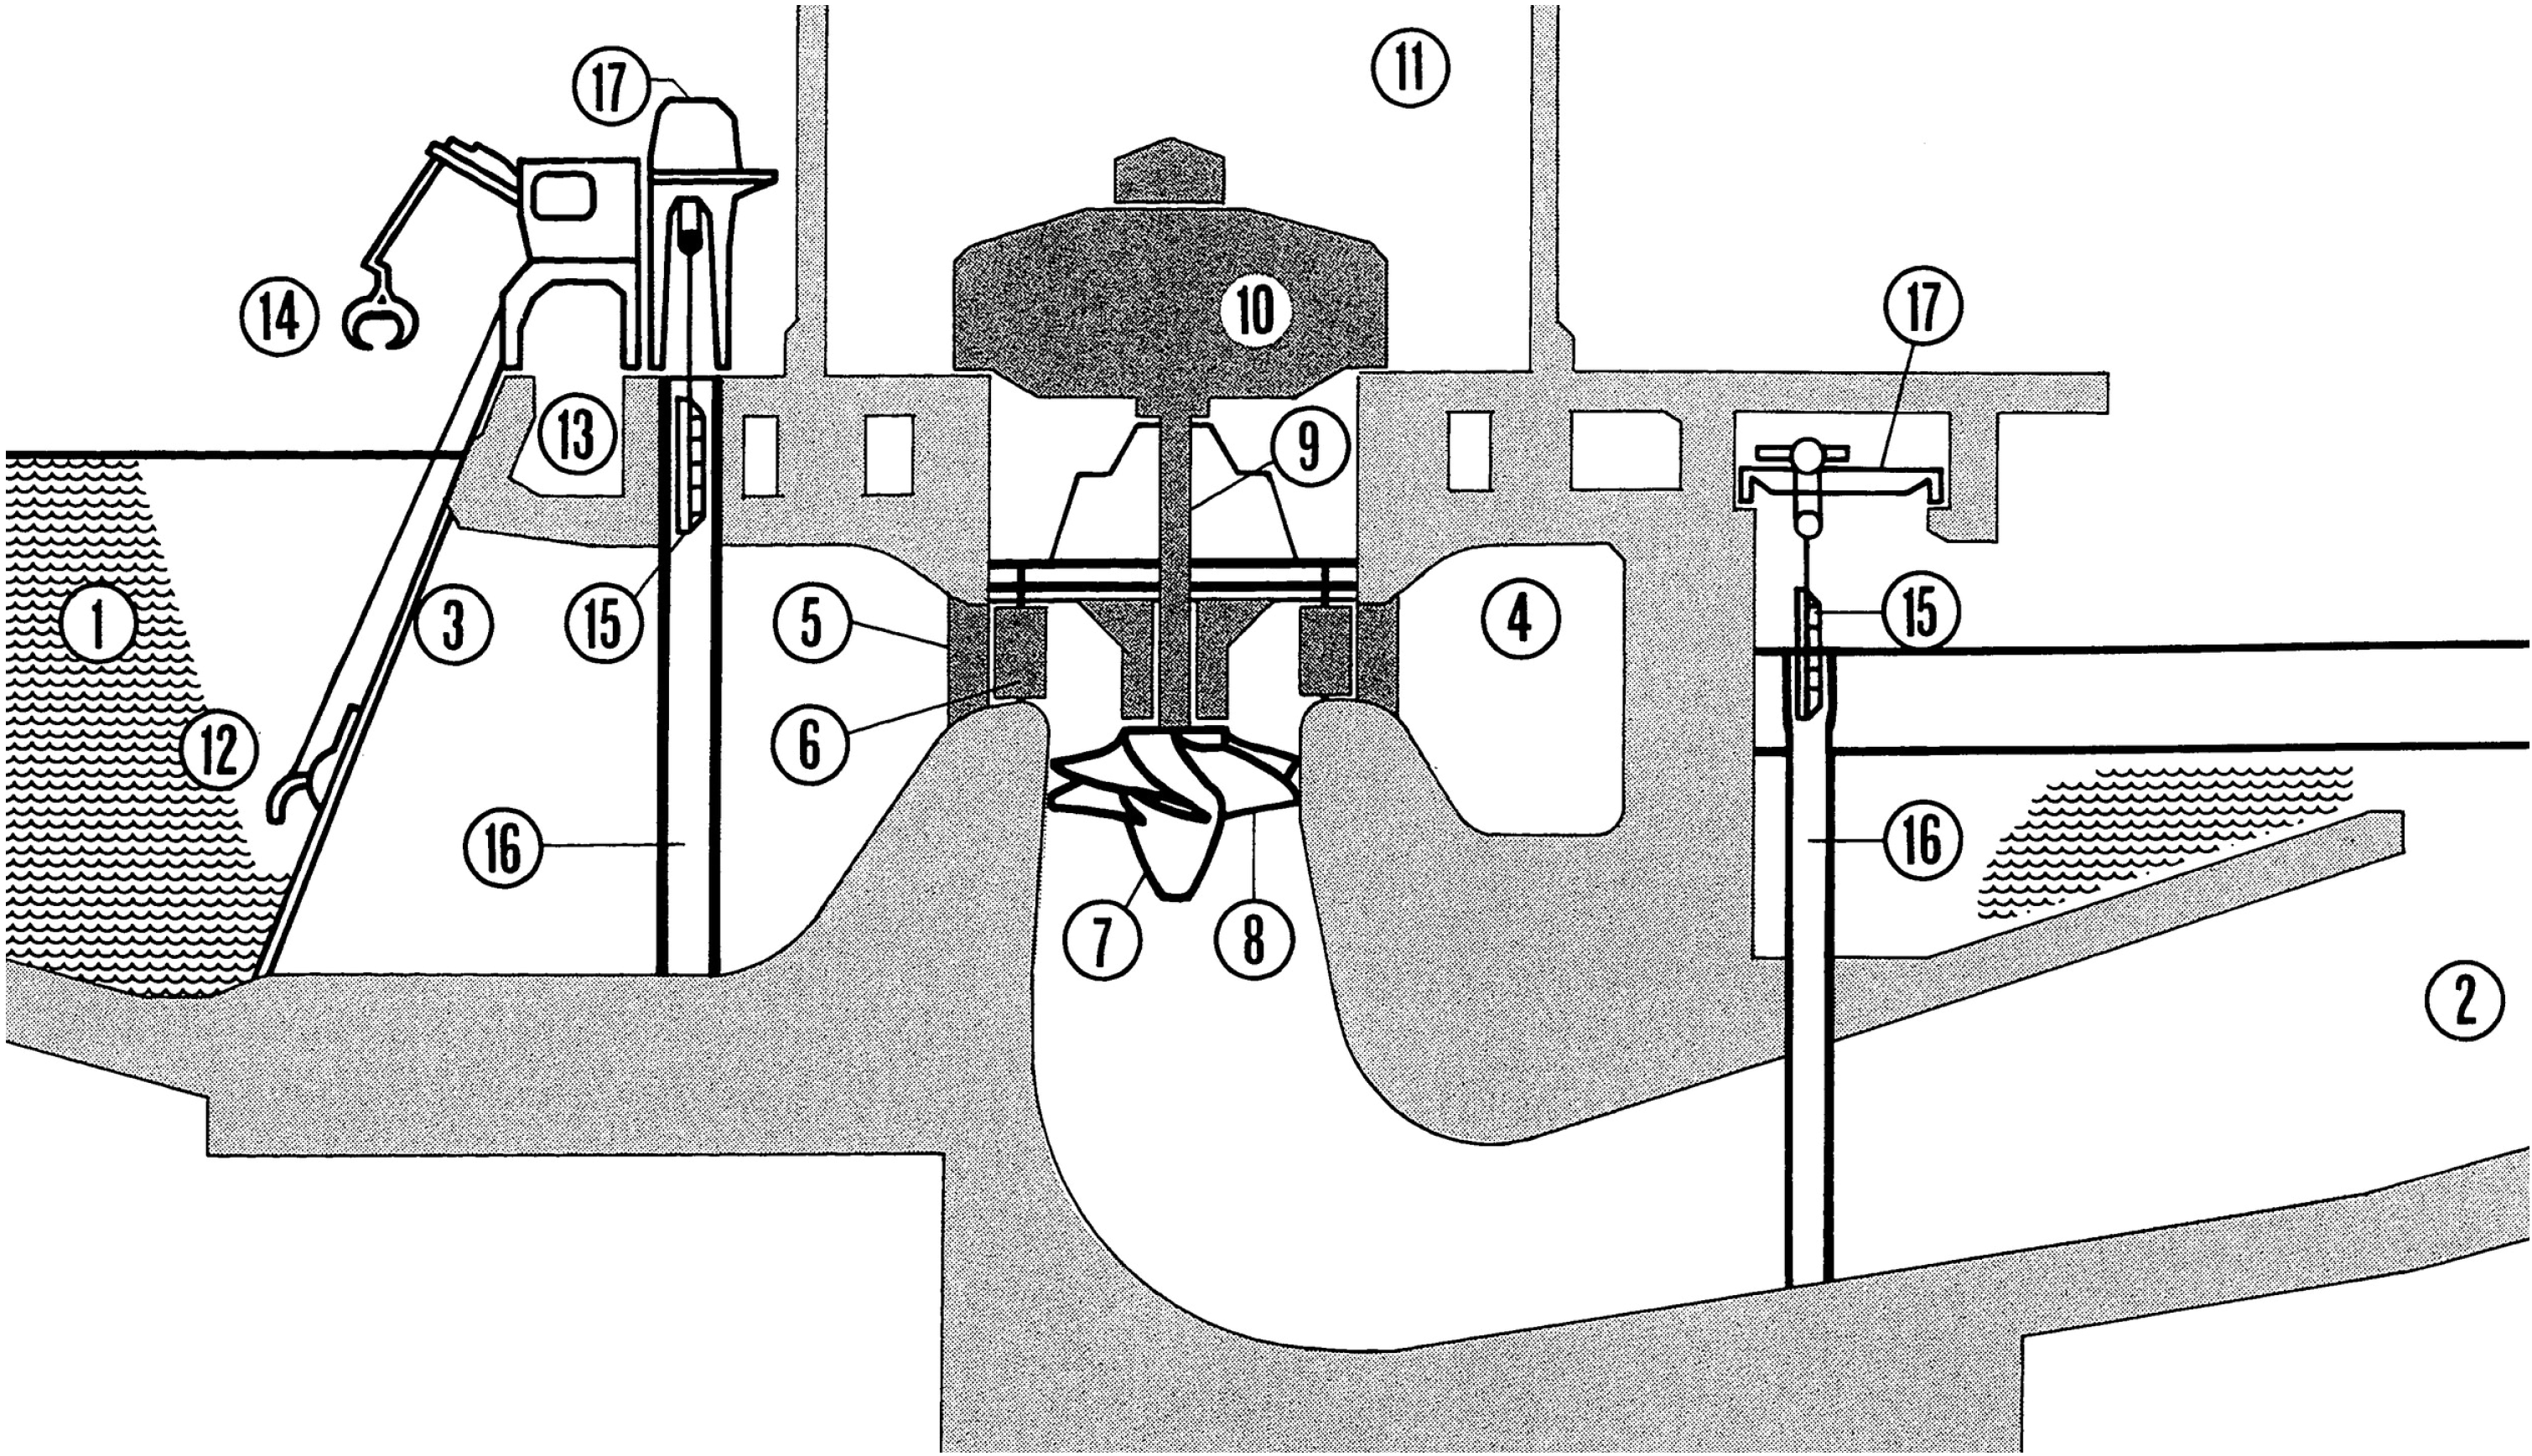
\includegraphics[width=0.95\columnwidth, align=c]{images/Laufwasserkraftwerke_Kaplanturbine_Vertikal.png}
\end{center}

\begin{minipage}[t]{0.38\columnwidth}
    \begin{tabular}{c l}
        1 & Oberwasser \\
        2 & Unterwasser \\
        3 & Rechen \\
        4 & Spirale \\
        5 & Stützschaufeln \\
        6 & Leitschaufeln \\
        7 & Laufrad \\
        8 & Laufradschaufeln \\
        9 & Saugrohr \\
    \end{tabular}
\end{minipage}
\hfill
\begin{minipage}[t]{0.58\columnwidth}
    \begin{tabular}{c l}
        10 & Generator \\
        11 & Maschinenhaus \\
        12 & Rechenreinigungsmaschine \\
        13 & Geschwemmselrinne \\
        14 & Zangengreifer \\
        15 & Dammbalken \\
        16 & Nuten für Dammbalken \\
        17 & Dammbalkenkran \\
           &  \\
    \end{tabular}
\end{minipage}



\subsection{LWK mit Rohrturbinen}

\begin{itemize}
    \item Turbine Horizontal verbaut
    \item bis 25m Fallhöhe
\end{itemize}

\begin{center}
    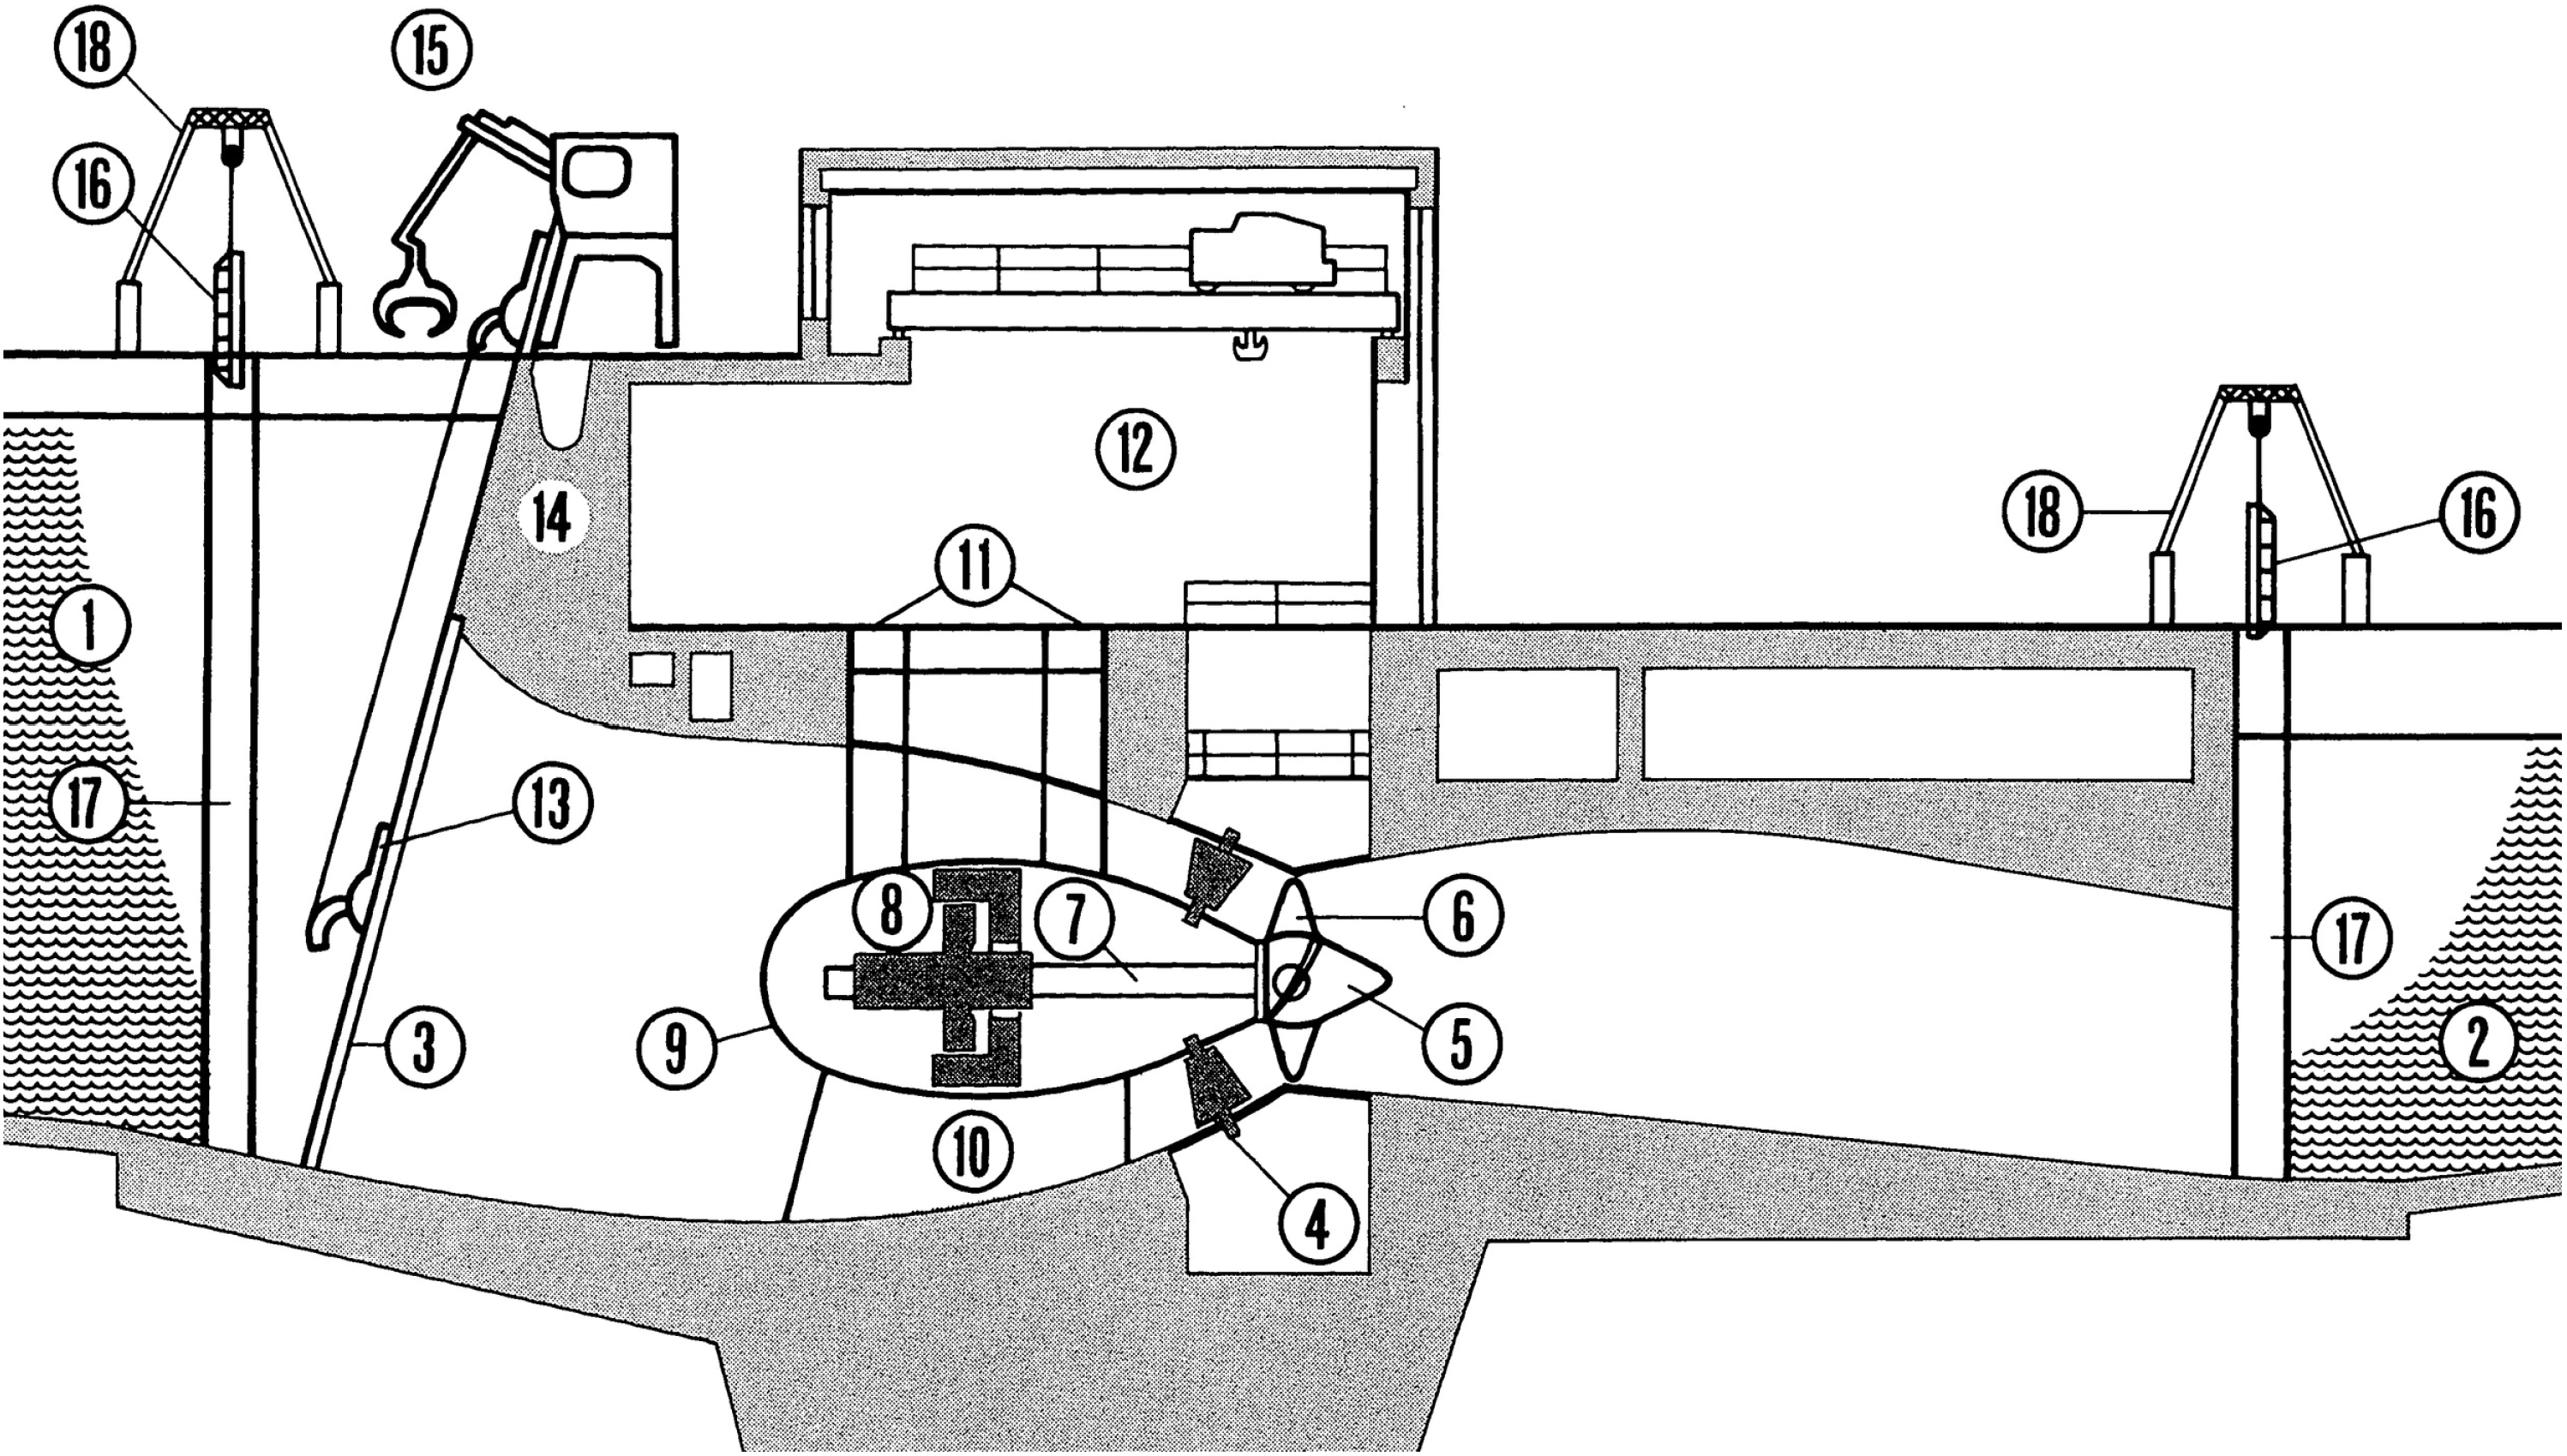
\includegraphics[width=0.95\columnwidth, align=c]{images/Laufwasserkraftwerke_Kaplanturbine_Horizontal.png}
\end{center}

\begin{minipage}[t]{0.38\columnwidth}
    \begin{tabular}{c l}
        1 & Oberwasser \\
        2 & Unterwasser \\
        3 & Rechen \\
        4 & Leitschaufeln \\
        5 & Laufrad \\
        6 & Laufradschaufeln \\
        7 & Turbinenwelle \\
        8 & Generator \\
        9 & Gehäuse \\
    \end{tabular}
\end{minipage}
\hfill
\begin{minipage}[t]{0.58\columnwidth}
    \begin{tabular}{c l}
        10 & Sockel \\
        11 & Einstiegsschächte \\
        12 & Maschinenhalle \\
        13 & Rechenreinigungsmaschine \\
        14 & Geschwemmselrinne \\
        15 & Zangengreifer \\
        16 & Dammbalken \\
        17 & Nuten für die Dammbalken \\
        18 & Dammbalkenkran \\
    \end{tabular}
\end{minipage}


\newcolumn
\subsection{LWK mit Strafloturbinen}

\begin{itemize}
    \item Weiterentwicklung der Rohrturbine
    \item Rotor Turbine und Generator bilden Einheit
\end{itemize}

\begin{center}
    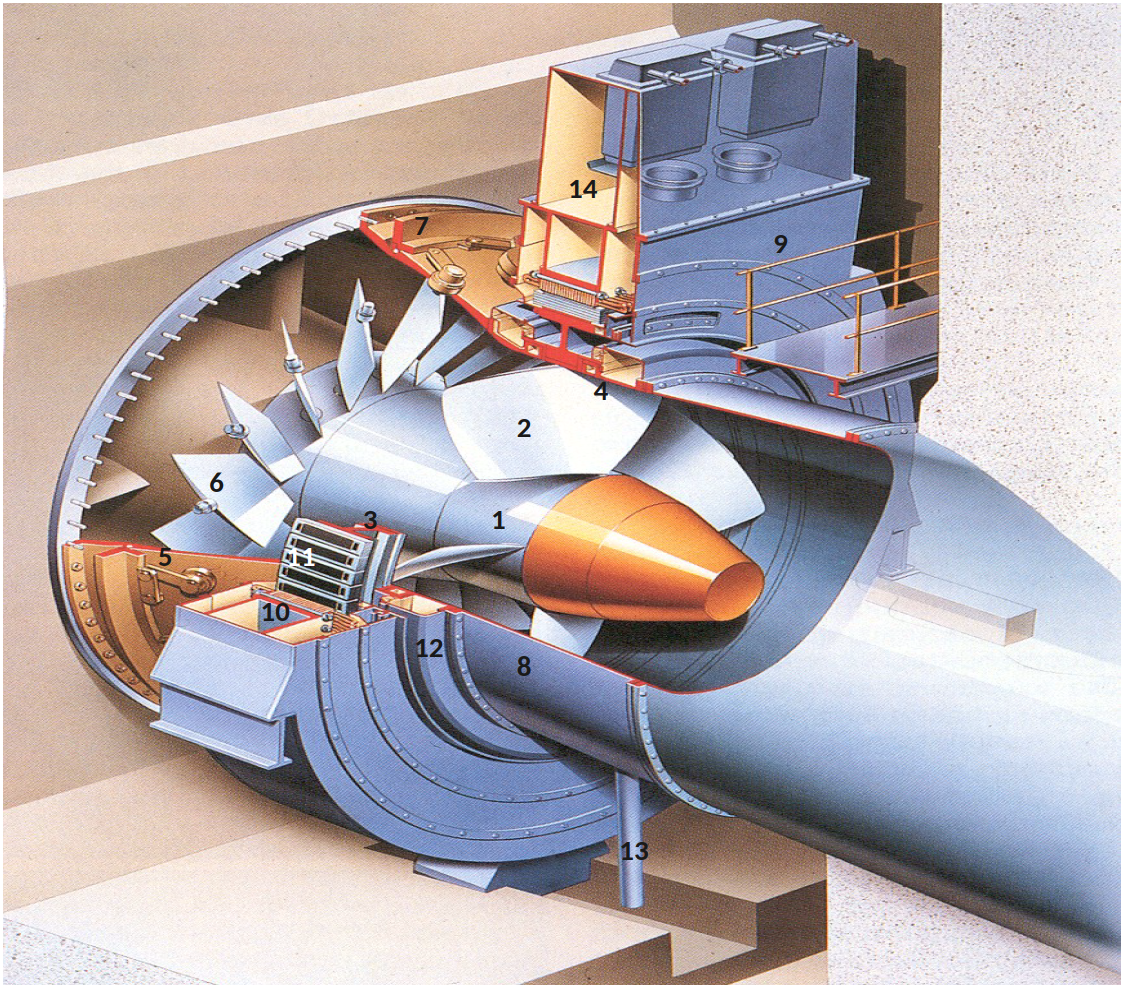
\includegraphics[width=0.95\columnwidth, align=c]{images/Laufwasserkraftwerke_mit_Strafloturbinen.png}
\end{center}

\begin{minipage}[t]{0.38\columnwidth}
    \begin{tabular}{c l}
        1 & Laufradnabe \\
        2 & Propellerblatt \\
        3 & Rotorring \\
        4 & Entlastungsring \\
        5 & Turbinengehäuse \\
        6 & Leitschaufel \\
        7 & Leitradverstellring \\
    \end{tabular}
\end{minipage}
\hfill
\begin{minipage}[t]{0.58\columnwidth}
    \begin{tabular}{c l}
        8 & Rohrleitung \\
        9 & Generator \\
        10 & Stator \\
        11 & Rotor \\
        12 & Ringdichtungs-Leckwasser-Kollektor \\
        13 & Leckwasserableitung \\
        14 & Kühler \\
    \end{tabular}
\end{minipage}

\subsection{Mitteldruckanlagen}

\begin{itemize}
    \item bis circa 50m Fallhöhe
    \item (<= 5 bar Druck)
\end{itemize}


\subsection{Hochdruck- (Speicher-) Anlagen}

\begin{itemize}
    \item ab circa 50m Fallhöhe
    \item (> 5 bar Druck, bis weit über 100 bar möglich)
\end{itemize}

\begin{center}
    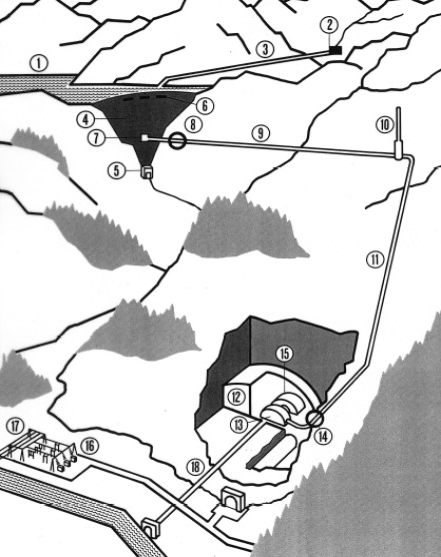
\includegraphics[width=0.95\columnwidth, align=c]{images/Hochdruckspeicheranlagen.png}
\end{center}

\begin{minipage}[t]{0.48\columnwidth}
    \begin{tabular}{c l}
        1 & Stausee \\
        2 & Wasserfassung \\
        3 & Freispiegelstollen (keine Druckleitung) \\
        4 & Staumauer \\
        5 & Grundablass (für kontrollierten Ablauf) \\
        6 & Hochwasserentlastung (= Überlauf) \\
        7 & Einlauf \\
        8 & Drosselklappe \\
        9 & Druckstollen \\
    \end{tabular}
\end{minipage}
\hfill
\begin{minipage}[t]{0.48\columnwidth}
    \begin{tabular}{c l}
        10 & Wasserschloss \\
        11 & Druckschacht \\
        12 & Zentrale \\
        13 & Turbine \\
        14 & Kugelschieber \\
        15 & Generator \\
        16 & Energieableitung, Transformatoren \\
        17 & Schaltanlage \\
        18 & Unterwasserstollen \\
    \end{tabular}
\end{minipage}



\subsection{Pumpspeicherkraftwerke PSW}

\begin{itemize}
    \item Pumpspeicherkraftwerk mit konventionellem Maschinensatz (Dreimaschinensatz)
    \item Wirkungsgrad der PSW: 65 – 80\%
\end{itemize}

\begin{center}
    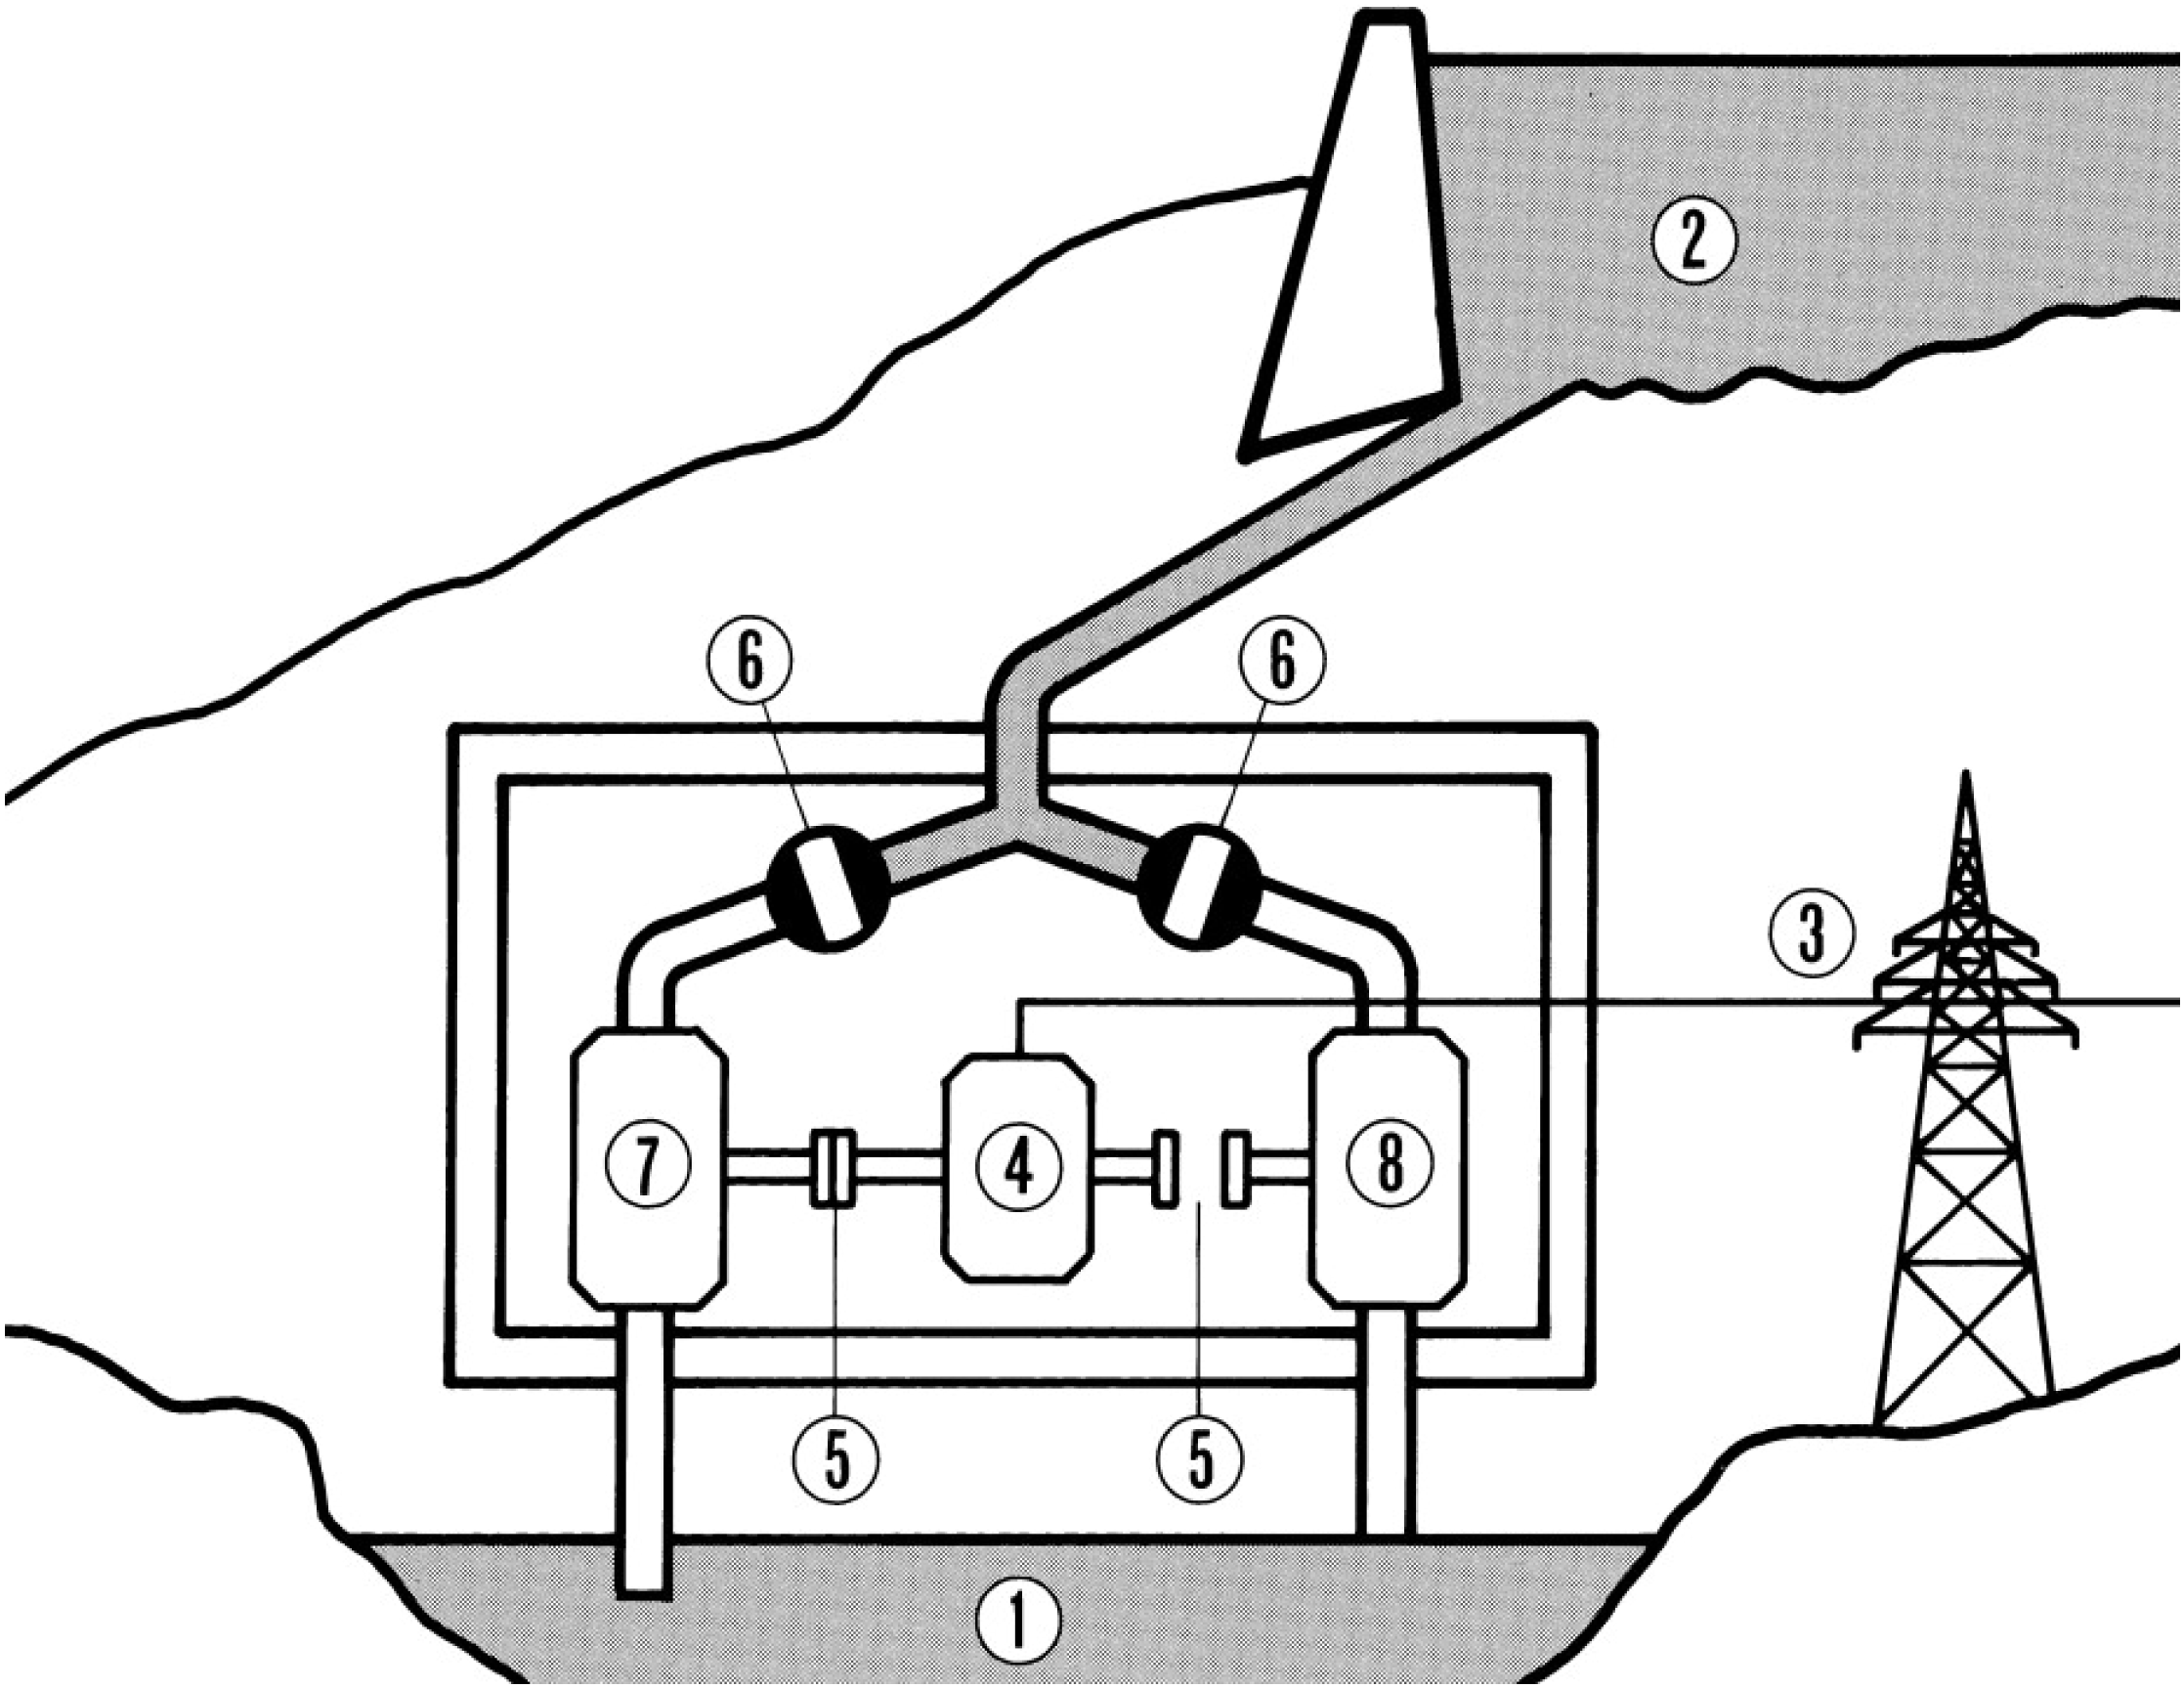
\includegraphics[width=0.95\columnwidth, align=c]{images/Pumpspeicherkraftwerke.png}
\end{center}

\begin{minipage}[t]{0.48\columnwidth}
    \begin{tabular}{c l}
        1 & Unteres Becken \\
        2 & Oberes Becken \\
        3 & Energieableitung, Stromleitung \\
        4 & Motorgenerator \\
    \end{tabular}
\end{minipage}
\hfill
\begin{minipage}[t]{0.48\columnwidth}
    \begin{tabular}{c l}
        5 & Kupplung \\
        6 & Kugelschieber \\
        7 & Pumpe \\
        8 & Turbine \\
    \end{tabular}
\end{minipage}


\subsection{Gezeitenkraftwerke}

\begin{itemize}
    \item Nutzung des Tidenhubs
    \item Früher meist mit Staudammbauweise (hohe Umwelteinwirkungen)
    \item Heute meist Meeresströmungs-Kraftwerk
    \item Grösste Europäische Anlage in Frankreich (240 MW)
\end{itemize}


\subsection{Wellenkraftwerk}

\subsubsection{Wellenkraftwerk mit Pneumatischer Kammer}
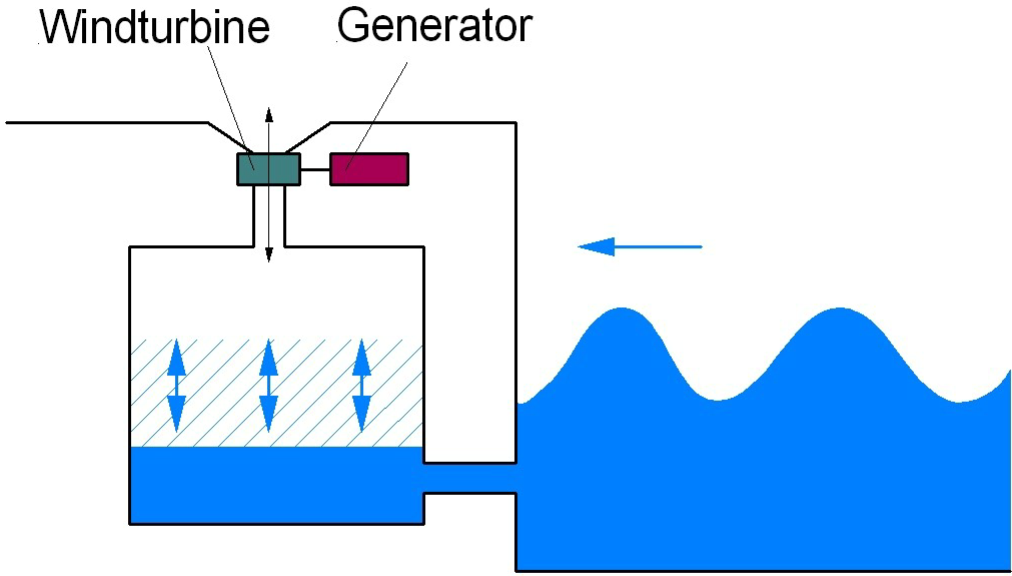
\includegraphics[width=0.65\columnwidth, align=c]{images/Wellenkraft mit Pneumatischer Kammer.png}


\subsubsection{Wellenkraftwerk mit Rampe}
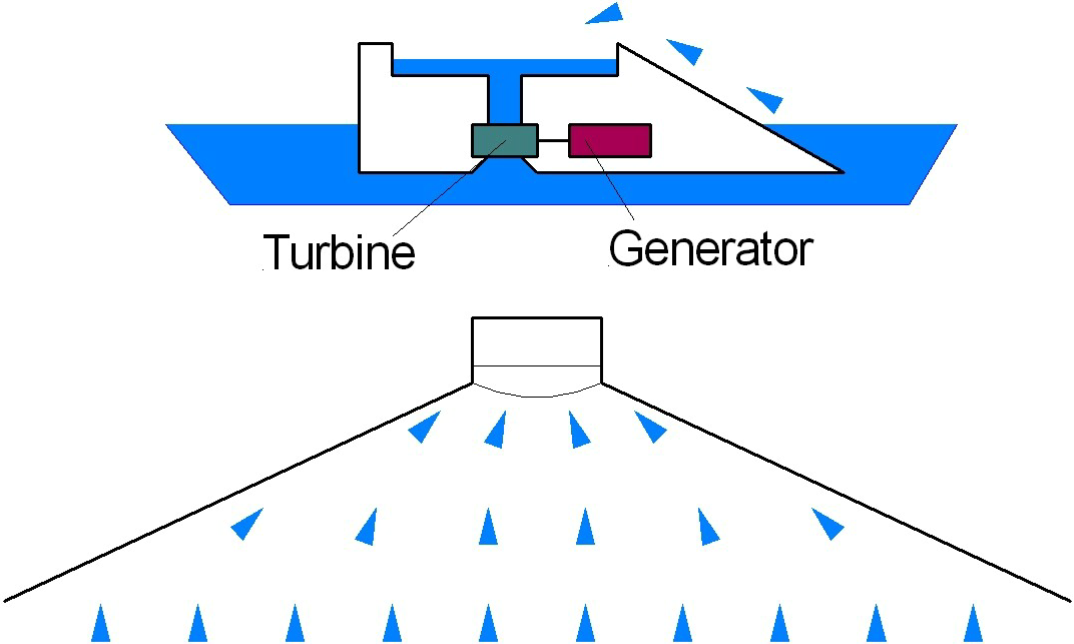
\includegraphics[width=0.65\columnwidth, align=c]{images/Wellenkraft mit Rampe.png}



\subsection{Wasserwirbelkraftwerk}

\begin{minipage}[c]{0.58\columnwidth}
    \begin{itemize}
    \item Für Kleinwasserkraft
    \item Geringe Fallhöhen und Durchfluss möglich:\\
    $h \geqq 0.5\text{m}$ und $Q \geqq 0.5 \frac{\text{m}^3}{\text{s}}$
    \item Geringerer Wirkungsgrad
    \item Besser Fischgängig
\end{itemize}
\end{minipage}
\hfill
\begin{minipage}[c]{0.38\columnwidth}
    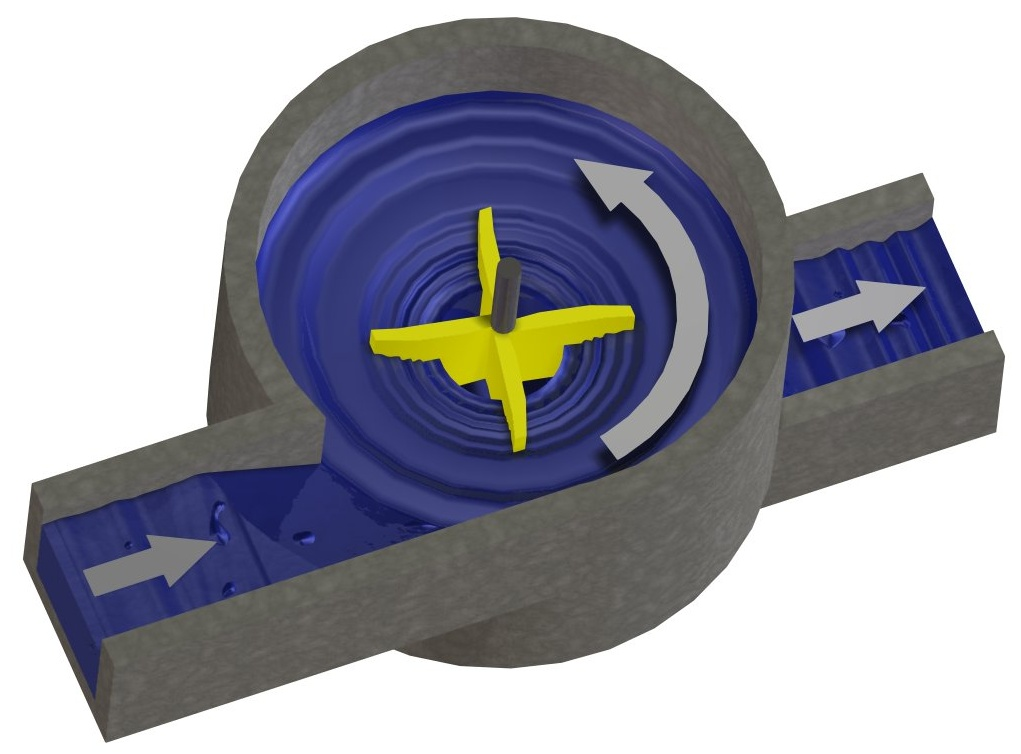
\includegraphics[width=0.65\columnwidth, align=c]{images/Wasserwirbelkraftwerk.jpg}
\end{minipage}
        %\newpage
\section{Turbinen Kenngrössen}
\subsection{Nettofallhöhe und Durchfluss}

\subsection{Hydraulische Leistung}

$\boxed{P_{\text{hyd}} = \rho \cdot Q \cdot g \cdot H_n}$

\renewcommand{\arraystretch}{1.2} % Erhöht Zeilenhöhe für bessere Lesbarkeit
\begin{tabular}{@{} l p {7cm} l @{}}
    $[P_{\text{hyd}}]$  & Hydraulische Leistung \dotfill & $W$ \\
    $[Q]$               & Nutzwassermenge \dotfill & $m^3/s$ \\
    $[H_n]$             & Nettofallhöhe \dotfill & $m$ \\
    $[\rho]$            & Dichte des Wassers ($\rho = 1000$) \dotfill & $\frac{kg}{m^3}$ \\
    $[g]$               & Erdbeschleunigung ($g = 9.81$) \dotfill & $\frac{m}{s^2}$ \\
\end{tabular}



\subsection{Mechanische Leistung an der Turbinenwelle}

$\boxed{P_{\text{mech}} = \omega \cdot M}$

\renewcommand{\arraystretch}{1.2} % Erhöht Zeilenhöhe für bessere Lesbarkeit
\begin{tabular}{@{} l p {6cm} l @{}}
    $[P_{\text{mech}}]$  & Mechanische Leistung   \dotfill & $W$ \\
    $[\omega]$           & Winkelgeschwindigkeit \dotfill & $\frac{\text{rad}}{s}$ \\
    $[M]$                & Drehmoment            \dotfill & $Nm$ \\
\end{tabular}


\subsection{Winkelgeschwindigkeit}

$\boxed{\omega = 2 \cdot \pi \cdot n}$

\renewcommand{\arraystretch}{1.2} % Erhöht Zeilenhöhe für bessere Lesbarkeit
\begin{tabular}{@{} l p {6cm} l @{}}
    $[\omega]$  & Winkelgeschwindigkeit \dotfill & $\frac{\text{rad}}{s}$ \\
    $[n]$       & Drehzahl              \dotfill & $\frac{1}{s}$ \\
\end{tabular}


\subsection{Betriebszustände der Maschinengruppe}
\textbf{(Maschinengruppe = Turbine/Pumpe + Generator/Motor)}

\begin{itemize}
    \item Inselbetrieb
    \item Parallelbetrieb, Verbundbetrieb
    \item Instationäre Vorgänge
    \begin{itemize}
        \item Anfahren und Abstellen
        \item Lastabwurf $\Rightarrow$ Überdrehzahl
    \end{itemize}
\end{itemize}

\textbf{Durchgangsdrehzahl $n_D$} (auch Schleuderdrehzahl genannt) $\Rightarrow$ höchste erreichbare Drehzahl ohne Last (z.B. bei Versagen des Generators)

Die Durchgangsdrehzahl ist eine Bemessungsgröße. Die Maschinengruppe darf bei der Durchgangsdrehzahl keinen Schaden erleiden.




















        %%%%%%%\input{sections/23_Thermische_Kraftwerke.tex}
        %\input{sections/25_Gasturbinenkraftwerke.tex}
        %\input{sections/30_Gas_und_Dampfturbinenkraftwerke.tex}
        %\input{sections/35_Kombianlagen_für_Kraft-und_Wärmekopplung.tex}
        %\section{Atomkraftwerk}

\subsubsection{Merkmale Nukleare Dampferzeugung}

\begin{outline}
  \1 Leistungsfähige Energiequelle
  \1 CO2 - freie Produktion elektrischer Energie
  \1 Aufwändige Technologie
  \1 Sicherheit
  \1 Tiefenlager radioaktiver Stoffe
  \1 Diskussion in Politik, Gesellschaft, Ethik
\end{outline}


\subsubsection{Kernprozesse für die Energiegewinnung}

\begin{outline}
  \1 Künstliche Kernspaltung schwerer Kerne (Fission)
    \2 → Kernkraftwerke 3. Generation
    \2 (Stand der Technik)
    
  \1 Umwandlung von schweren Kernen in gut spaltbare Kerne im Brutprozess (Konversion)
    \2 → Kernkraftwerke 4. Generation
    \2 (in Entwicklung)
    
  \1 Verschmelzung leichter Kerne zu einem Kern (Fusion)
    \2 → Grundlagenforschung in Bearbeitung
\end{outline}


\subsection{Kernphysikalische Grundlagen}

$\boxed{A = Z + N}$ \quad Nuklid-Schreibweise: $\boxed{\text{\ce{^{A}_{Z}Element}} }$ \quad \text{z.\,B.} \quad \text{\ce{^{235}_{92}U}}

\vspace{1em}
\renewcommand{\arraystretch}{1.2}
\begin{tabular}{@{} l p{6cm} l @{}}
    $[A]$ & Anzahl Kerneteilchen eines Atoms \dotfill & $-$ \\
    $[Z]$ & Anzahl Protonen (Kernladungszahl) \dotfill & $-$ \\
    $[N]$ & Anzahl Neutronen \dotfill & $-$ \\
\end{tabular}



\subsection{Spaltung schwerer Kerne}

\begin{outline}
    \1 Spaltung schwerer Kerne
    \1 Einige Isotope besitzen die Eigenschaft, dass sie beim Beschießen mit langsamen Neutronen diese im Kern absorbieren und in zwei Tochterkerne zerfallen, wobei gleichzeitig 2–3 Neutronen frei werden.

    \vspace{0.15cm}

    $\boxed{
    \ce{^{235}_{92}U + ^{1}_{0}n \rightarrow  ^{89}_{36}Kr + ^{144}_{56}Ba + 3 ^{1}_{0}n + 200MeV}
    }$

    \vspace{0.15cm}

    \1 Bindungsenergie wird dabei frei.\\
        Im Mittel sind dies: 
        \textbf{200 MeV = $\bm{3{,}2 \cdot 10^{-11}}$ Ws pro Spaltung}
    \1 Die „schnellen“ Neutronen müssen abgebremst werden ($\Rightarrow$  thermische Neutronen), so dass der Prozess nicht abbricht.\\
    Dies geschieht mit einem Moderator wie „leichtes“ Wasser oder Graphit.
    \1 Werden genügend thermische Neutronen zur Verfügung gestellt, hält sich durch eine Kettenreaktion der Spaltungsprozess selbst aufrecht.
\end{outline}


\crd{To be continued ...}





















        %\section{Windenergie}


\subsection{Windeleistung}

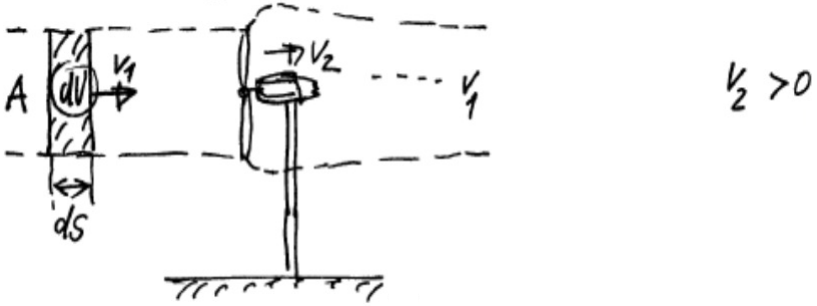
\includegraphics[width=0.95\columnwidth, align=c]{images/WEK_Leistungs-und_Drehzahlregelung.png}

$
\boxed{
P_{\text{max}} = \frac{dW}{dt} = \frac{A \cdot \rho_{\text{Luft}}}{2} \cdot v_1^3
}
\quad
\boxed{
P_W = c_P \cdot \frac{A \cdot \rho_{\text{Luft}}}{2} \cdot v_1^3
}
$ \quad Achtung! $v_1$ ist hoch 3!


\renewcommand{\arraystretch}{1.2}
\begin{tabular}{@{} l p{8cm} l @{}}
    $[P_{\text{max}}]$ & Theoretische Windleistung \dotfill & $W$ \\
    $[P_W]$            & Effektiv nutzbare praktische Windleistung \dotfill & $W$ \\
    $[c_P]$            & Leistungsbeiwert, $c_P = 0.4 ... 0.5$ \dotfill & $-$ \\
    $[A]$              & Rotorfläche (projizierte Fläche senkrecht zur Strömung) \dotfill & $m^2$ \\
    $[\rho_{\text{Luft}}]$ & Dichte Luft, $\approx 1{,}29 \, \frac{kg}{m^3}$ \dotfill & $\frac{kg}{m^3}$ \\
    $[v_1]$            & Anströmgeschwindigkeit des Windes \dotfill & $\frac{m}{s}$ \\
\end{tabular}



\section{Windenergiekonverter (WEK)}
\subsection{Netzkopplung}

DU = Direktumrichter, ZKU = Zwischenkreis-Umrichter\\

\subsubsection{Direkte Netzkopplung mit ASM}
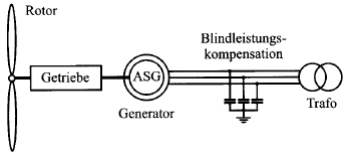
\includegraphics[width=0.6\columnwidth]{images/Direkte Netzkopplung mit ASM.png}

\subsubsection{Direkte Netzkopplung mit SM}
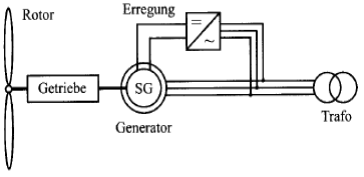
\includegraphics[width=0.6\columnwidth]{images/Direkte Netzkopplung mit SM.png}

\subsubsection{Direkte Netzkopplung mit ASM und DU im Läufer}
\includegraphics[width=0.6\columnwidth]{images/Direkte Netzkopplung mit ASM und Direktumrichter im Läufer.png}

\subsubsection{Direkte Netzkopplung mit SM über Gleichstromzwischenkreis}
\begin{itemize}
    \item variable Drehzahl
\end{itemize}

\vspace{0.1cm}

\includegraphics[width=0.6\columnwidth]{images/Direkte Netzkopplung mit SM über einen Gleichstromzwischenkreis, variable Drehzahl.png}

\subsubsection{Direkte Netzkopplung mit ASM und ZKU im Läufer}

\begin{itemize}
    \item übersynchrone Strorichter-Kaskade
    \item variable Drehzahl
\end{itemize}

\vspace{0.1cm}

\includegraphics[width=0.6\columnwidth]{images/Direkte Netzkopplung mit ASM und Zwischenkreis-umrichter im Läufer.png}
















        %\section{Netze Allgemein}


\subsubsection{Stromnetz früher}

\begin{center}
    \includegraphics[width=0.95\columnwidth, align=c]{images/Aufgabe_des_Netzes_früher.jpg}
\end{center}


\subsubsection{Stromnetz heute}

\begin{center}
    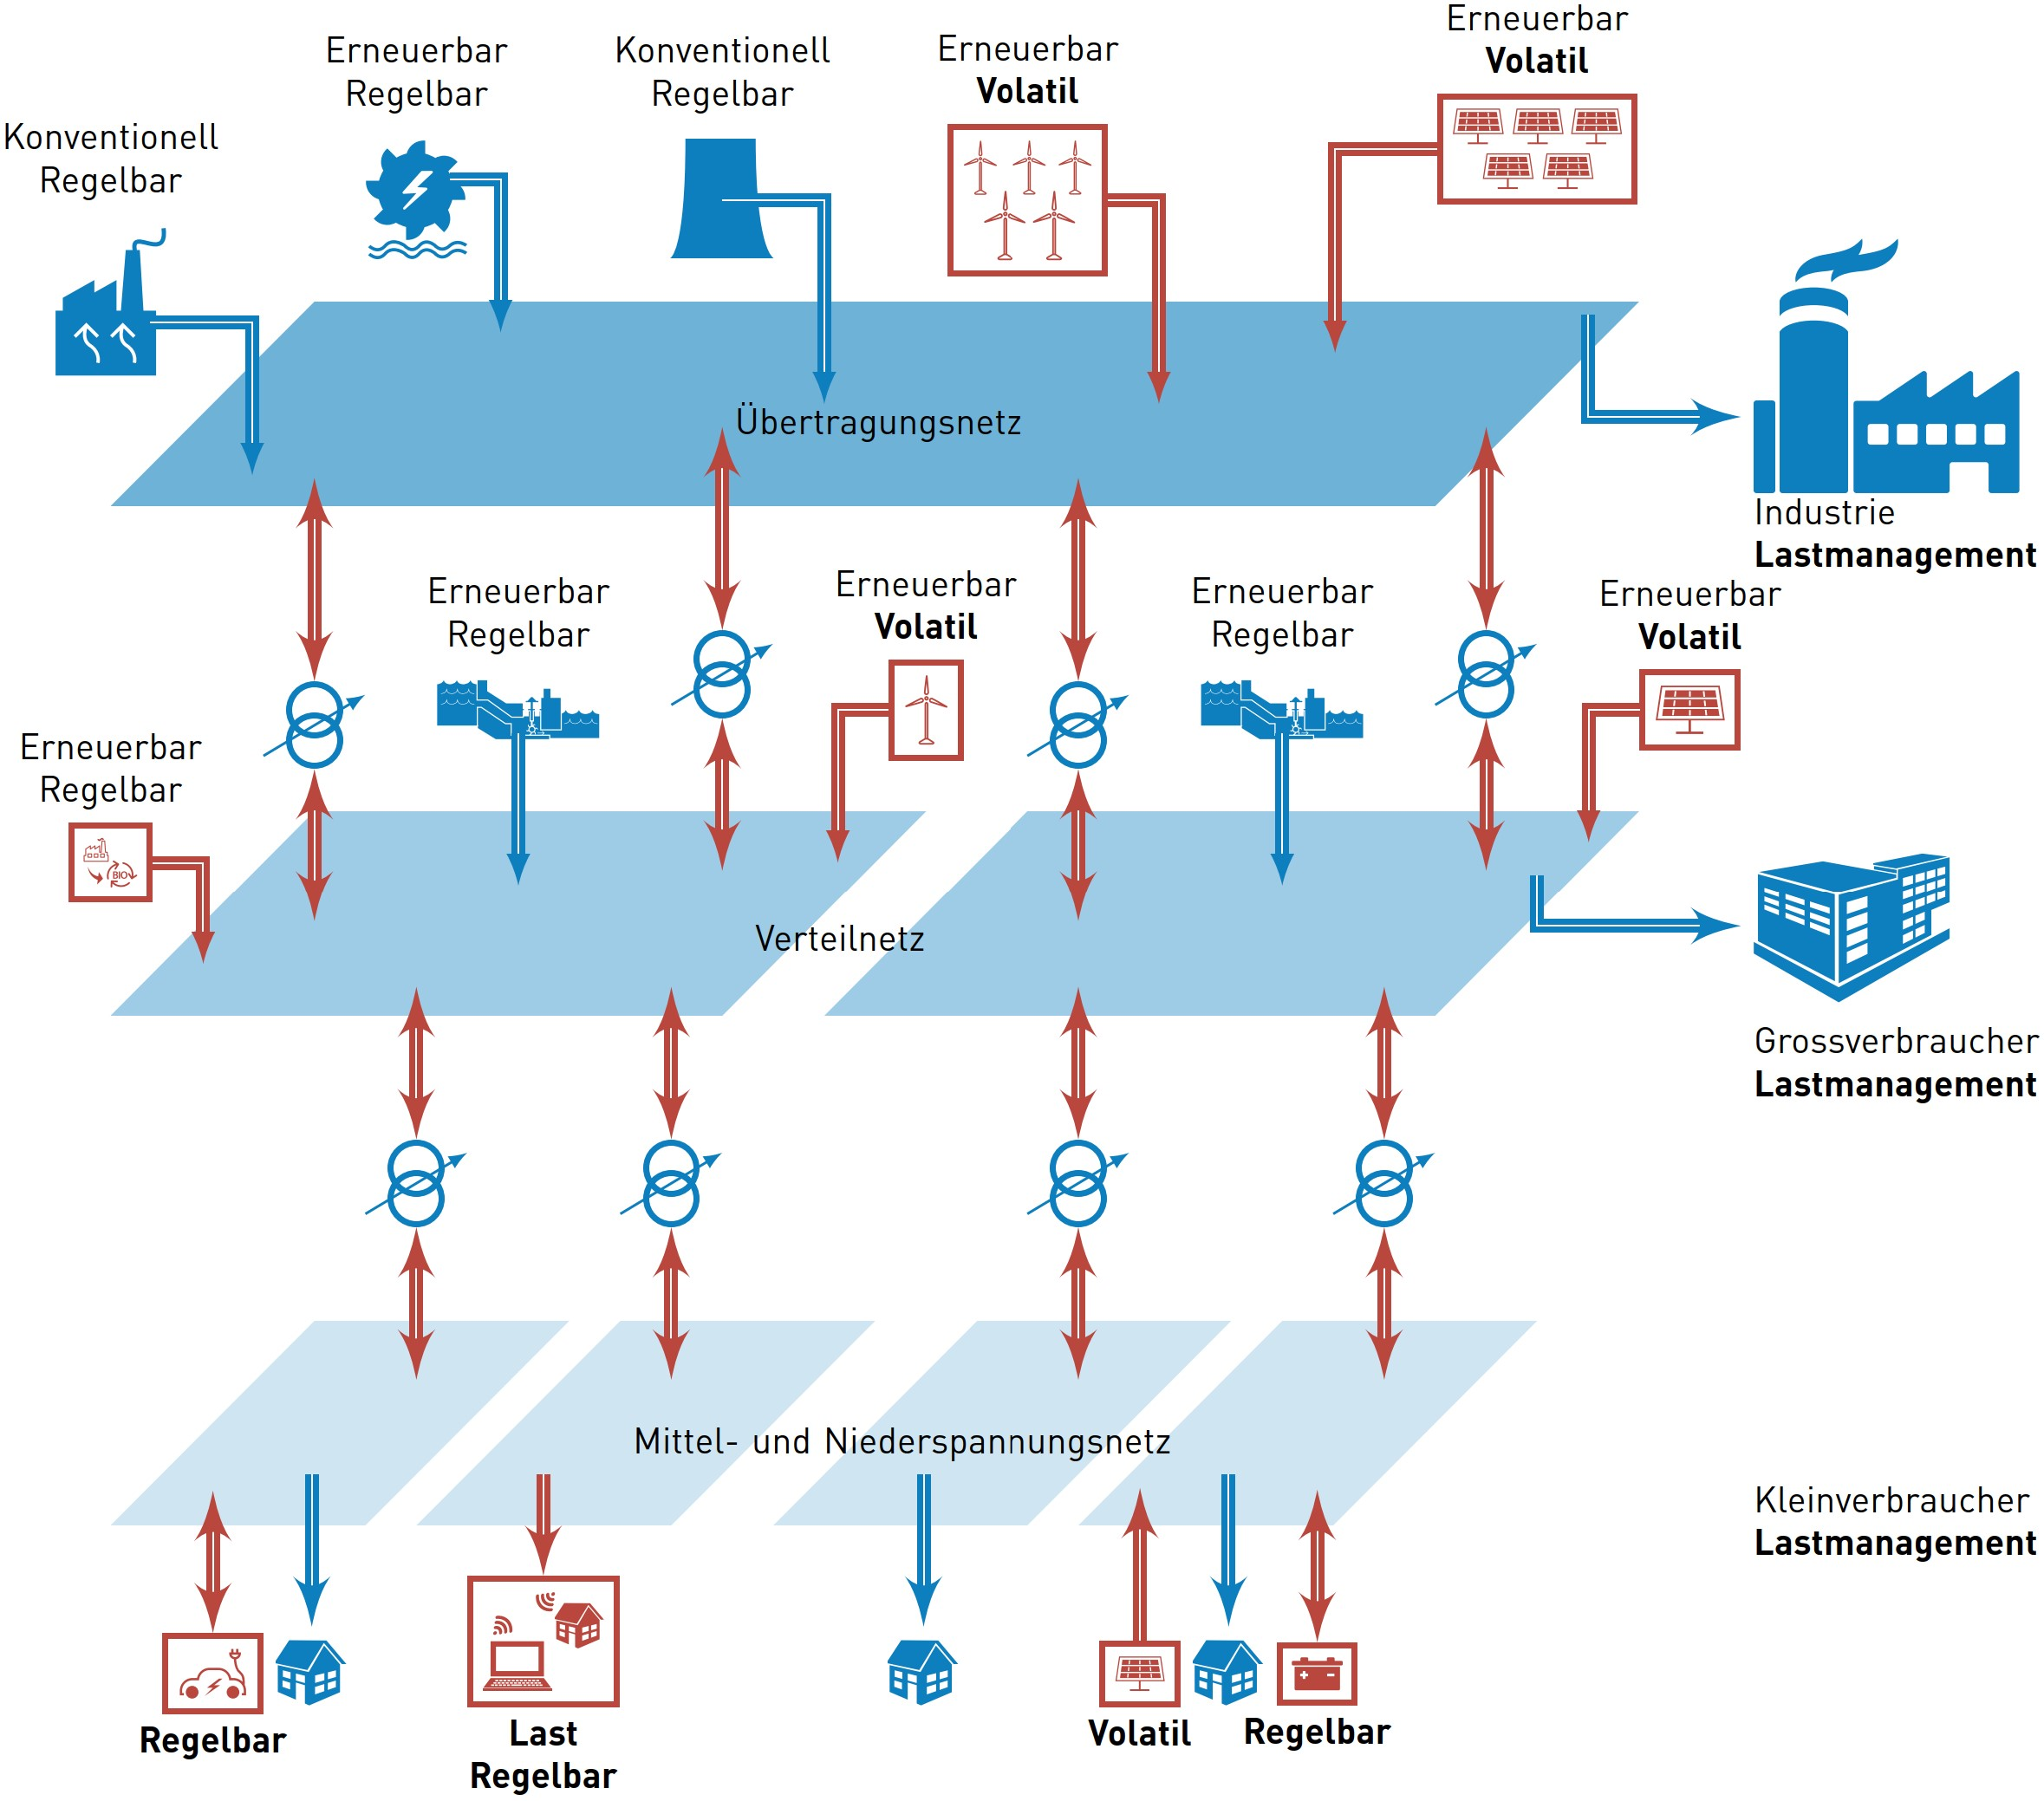
\includegraphics[width=0.95\columnwidth, align=c]{images/Aufgabe_des_Netzes_heute.jpg}
\end{center}

\subsection{Interessen der Erzeuger}

\begin{itemize}
    \item \textbf{Erzeuger}
    \begin{itemize}
        \item Freier Netzzugang
        \item Hohe Verfügbarkeit: produzierte Leistung kann jederzeit abgeführt werden
        \item Geringe Kosten
    \end{itemize}
    \item \textbf{Verbraucher}
    \begin{itemize}
        \item Netzanschluss
        \item Hohe Versorgungssicherheit und -qualität
        \item Geringe Kosten
    \end{itemize}
\end{itemize}


\subsection{Anforderungen an das Stromnetz}

\begin{itemize}
    \item Hohe Verfügbarkeit
    \item Hohe Versorgungsqualität
    \item Sicherheit
    \item Wirtschaftlichkeit
    \item Diskriminierungsfreiheit
    \item Transparenz
\end{itemize}



        %\section{Netzebenen}

\begin{center}
    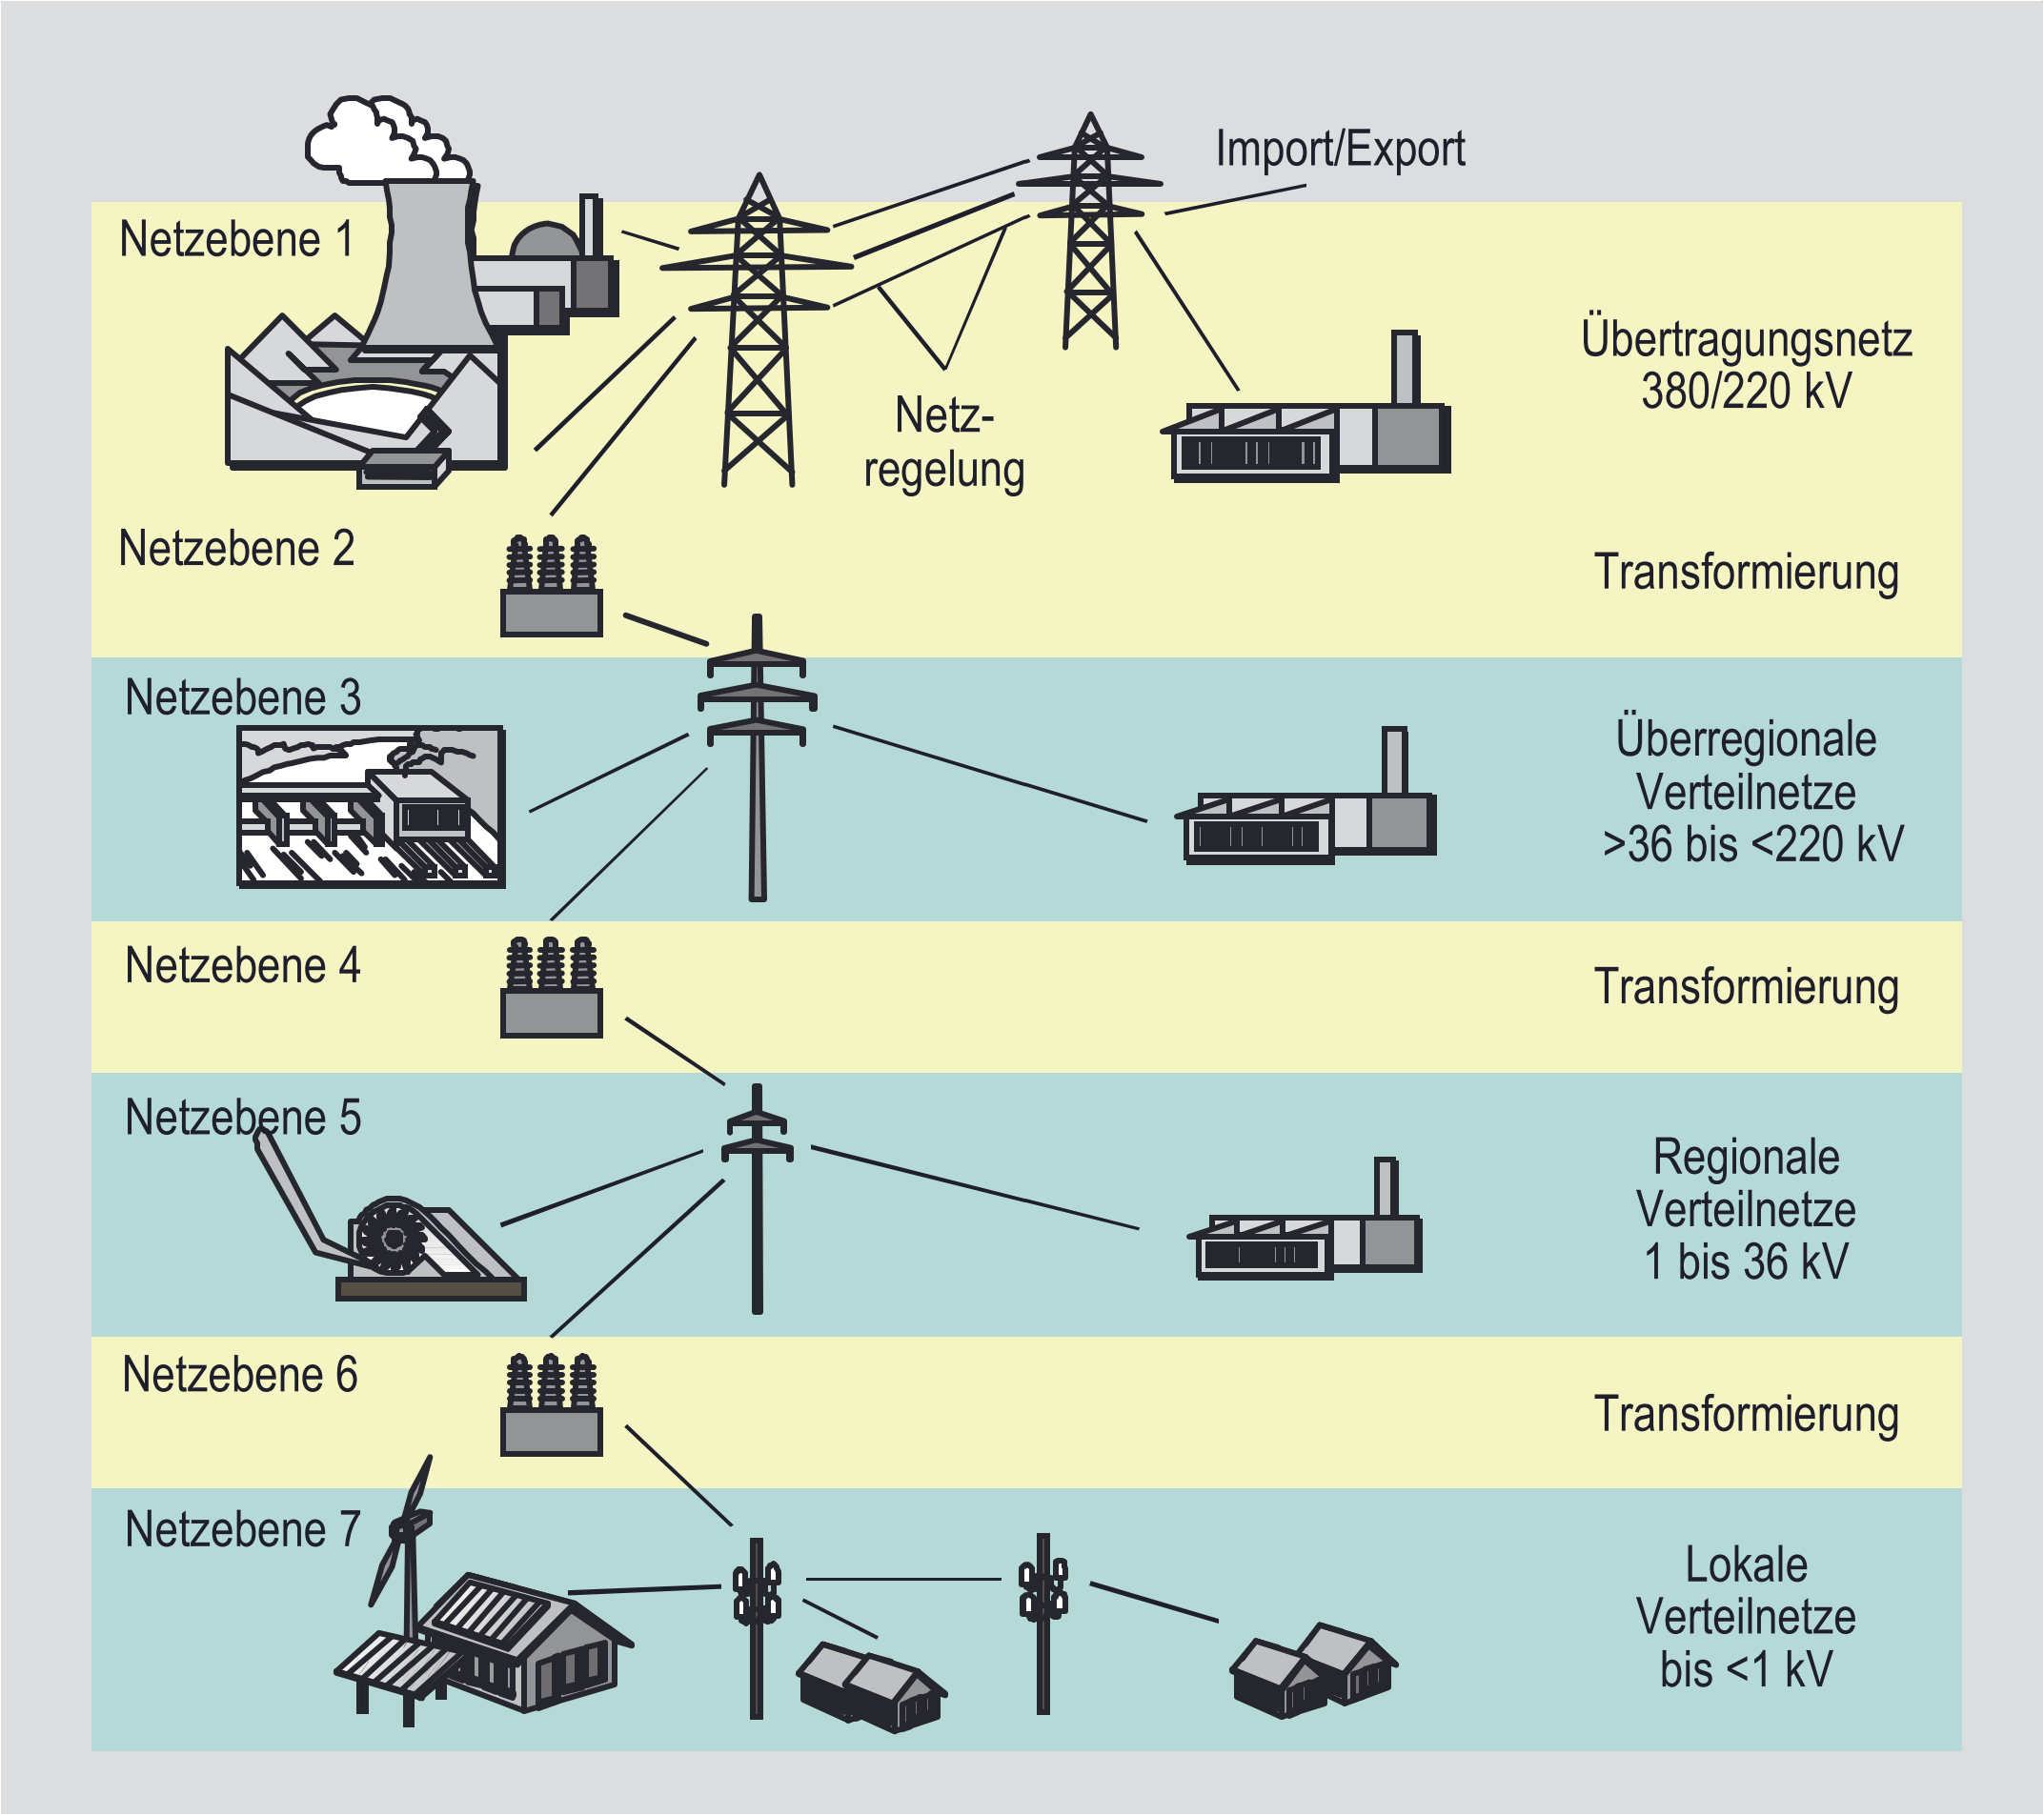
\includegraphics[width=0.95\columnwidth, align=c]{images/Netzebenen_1.png}
\end{center}

\begin{tabular}{>{\bfseries}l l l}
    \toprule
    Spannungsebene & Spannungsbereich & Leistung \\
    \midrule
    Höchstspannung   & 380 kV, 220 kV         & > 300 MVA \\
    Hochspannung     & 150 kV bis 50 kV       & < 100 MVA \\
    Mittelspannung   & 36 kV bis 6 kV         & < 30 MVA \\
    Niederspannung   & 0{,}4 kV               & < 1 MVA \\
    \bottomrule
\end{tabular}

\subsection{NE1: Übertragungsnetz}

\begin{itemize}
    \item 380 kV und 220 kV
    \item Zweck
    \begin{itemize}
        \item Abtransport der großen Kraftwerksleistungen (typ. > 300 MVA)
        \item Versorgung der Verteilnetze
        \item Weiträumiger Energietransport
        \item Internationaler Verbundbetrieb, Energieaustausch
    \end{itemize}
    \item \textbf{Ausdehnung:} national, international
    \item \textbf{Topologie:} (stark) vermaschtes Netz
    \item \textbf{Technologie:} fast ausschließlich Freileitungen
\end{itemize}

\subsubsection{Schweizer Stromübertragungsnetz (Daten 2014)}

\begin{center}
    \includegraphics[width=0.95\columnwidth, align=c]{images/Schweizer_übertragungsnetz.png}
\end{center}

\begin{itemize}
    \item Gesamtlänge Übertragungsnetz Inland: 6700 km
    \begin{itemize}
        \item Länge 380 kV: 1780 km
        \item Länge 220 kV: 4920 km
    \end{itemize}
    
    \item Gesamtzahl Leitungen im Übertragungsnetz: 246
    \begin{itemize}
        \item Leitungen 380 kV: 48
        \item Leitungen 220 kV: 198
    \end{itemize}
    
    \item Anzahl Netzübergänge in das Ausland: 41
\end{itemize}

\subsubsection{Entso-E}

\begin{center}
    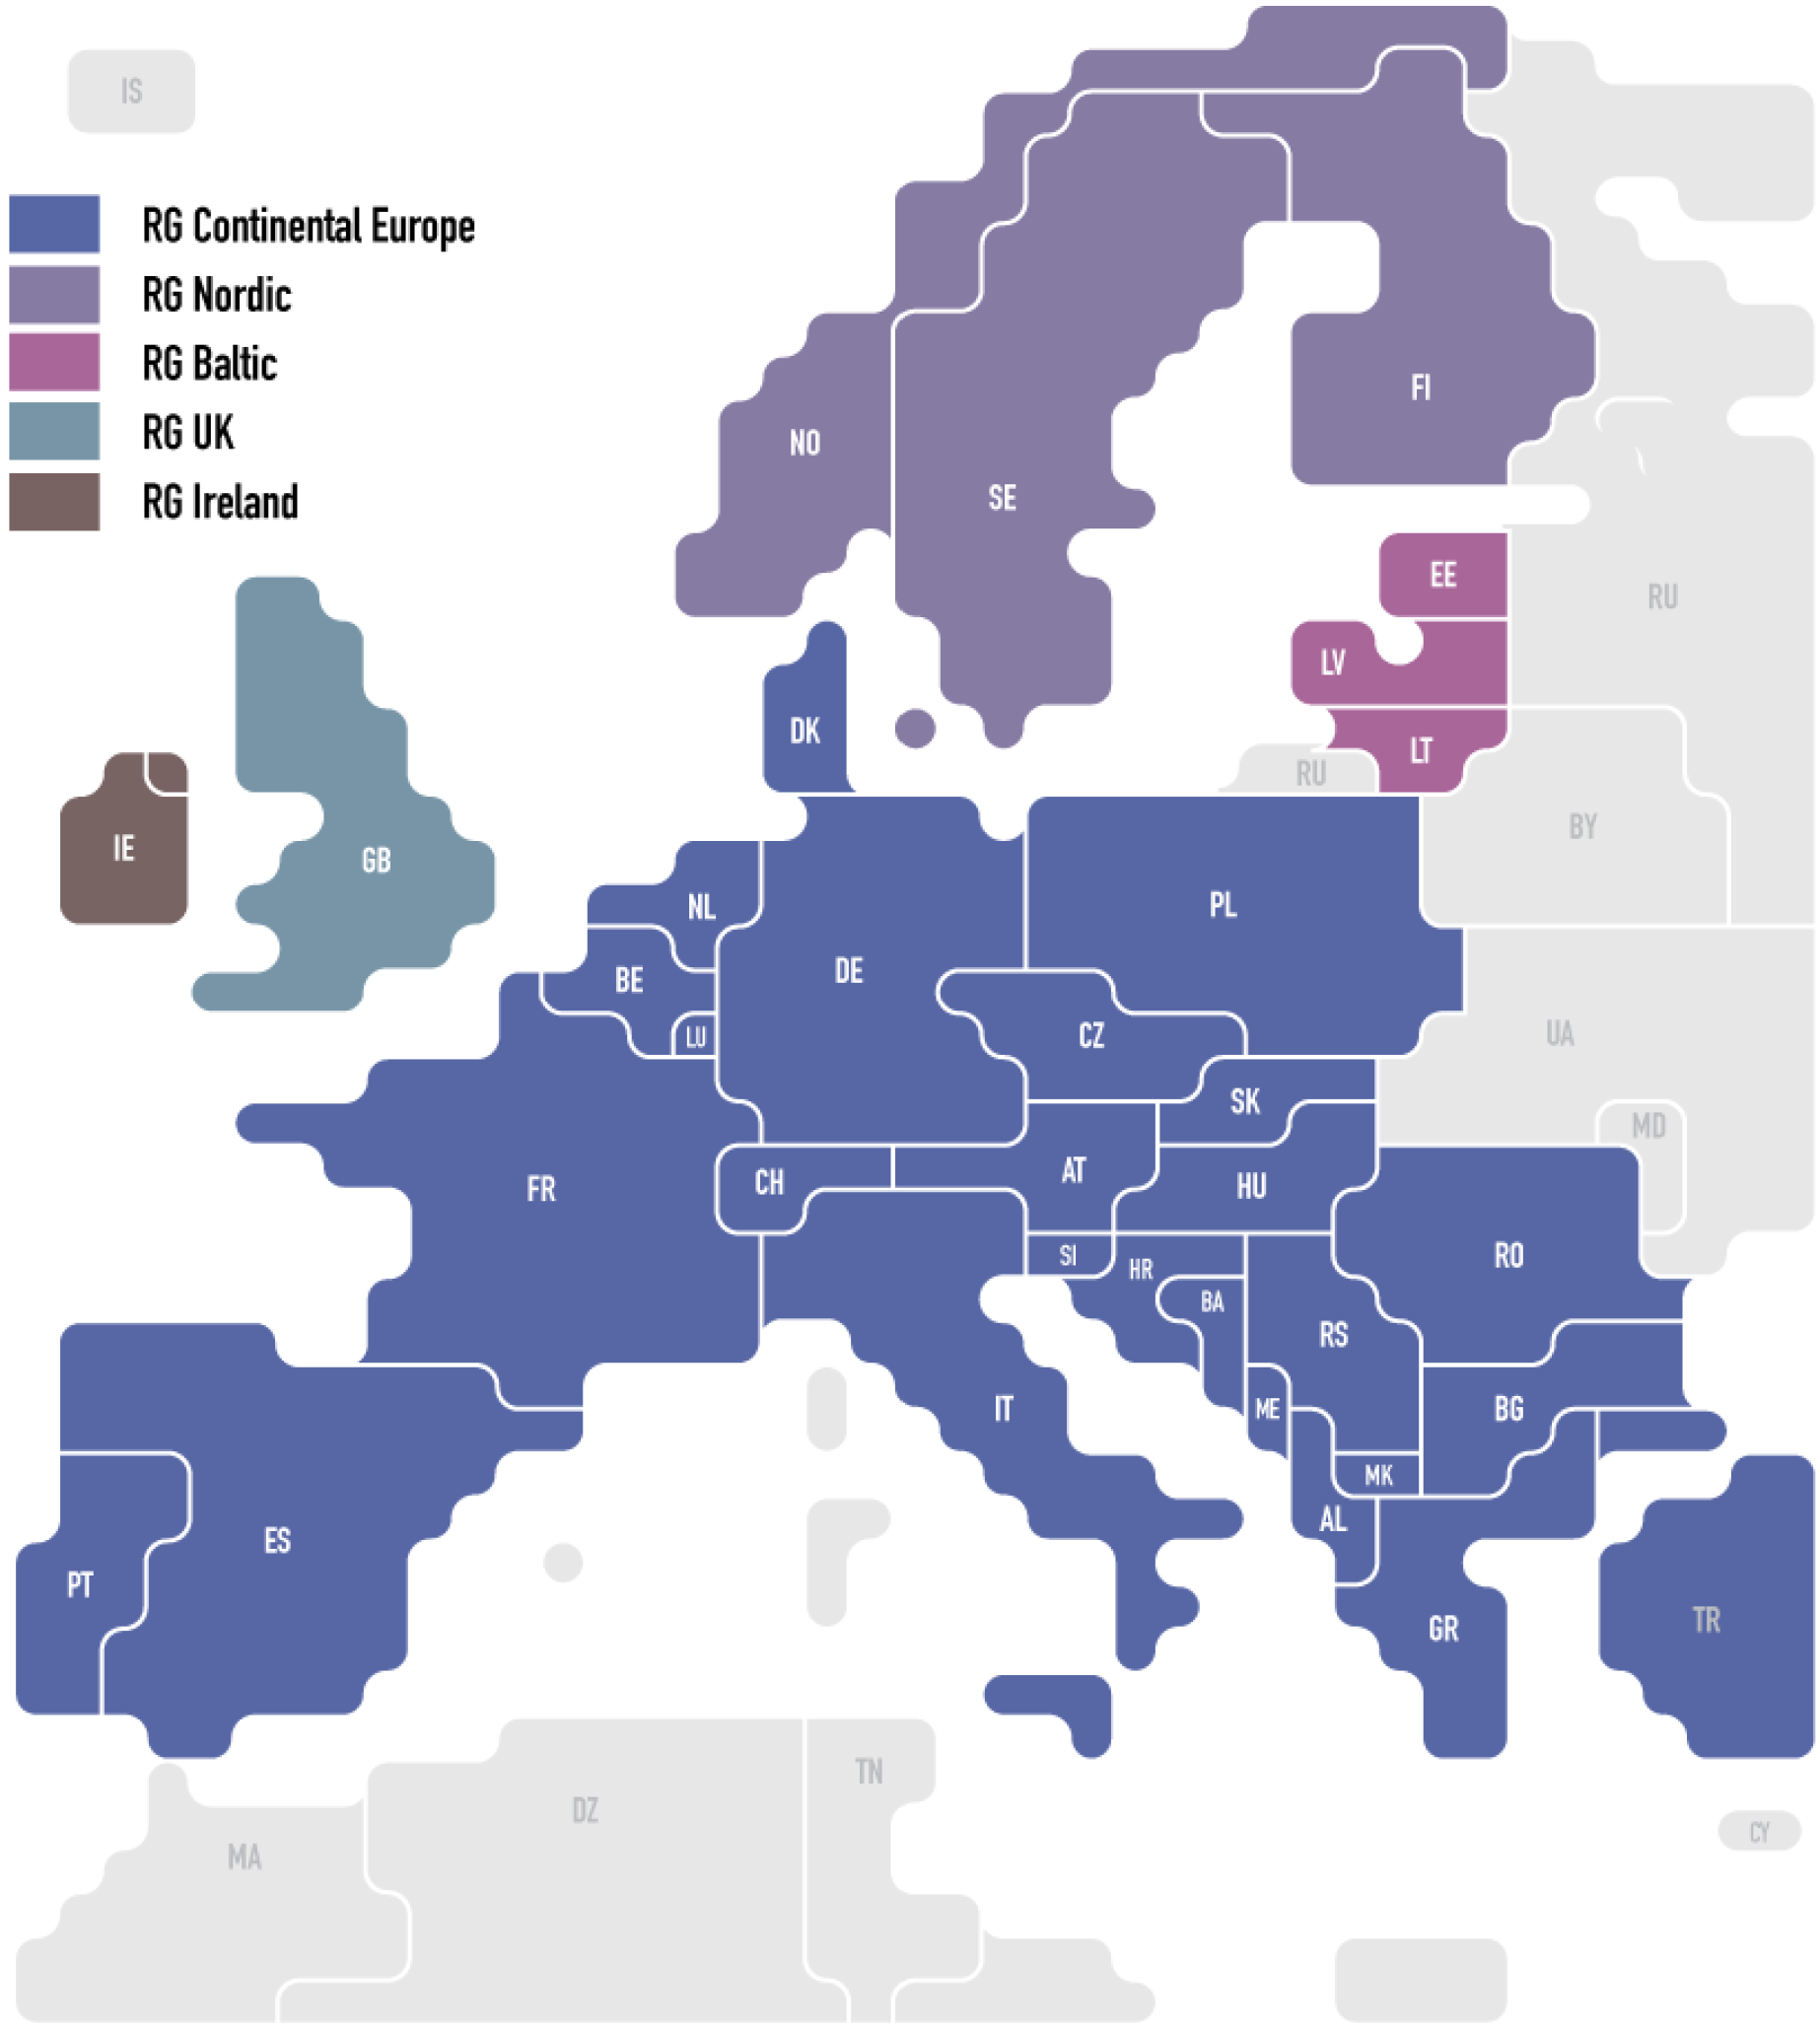
\includegraphics[width=0.95\columnwidth, align=c]{images/Entso_E.png}
\end{center}

\begin{itemize}
    \item koordinierter Systembetrieb
    \item koordinierte Marktlösungen
    \item koordinierte Systementwicklung
\end{itemize}




\subsection{NE3: Überregionales Verteilnetz}

\begin{itemize}
    \item 150 kV, 132 kV, 60 kV
    \item Zweck
    \begin{itemize}
        \item Abtransport mittlerer Kraftwerksleistungen (typ. 100 MVA)
        \item Anschluss großer Industriekunden
        \item Überregionale Verteilung
    \end{itemize}
    \item Ausdehnung: mehrere Kantone
    \item Topologie: (leicht) vermaschtes Netz oder Ringnetz
    \item Technologie: vorwiegend Freileitungen
\end{itemize}

\subsection{NE5: Verteilnetz}


\begin{itemize}
    \item 20 kV, 10 kV
    \item Zweck
    \begin{itemize}
        \item Abtransport kleiner Kraftwerksleistungen (\(< 30\,\text{MVA}\))
        \item Anschluss von Industrie- und Gewerbekunden
        \item Regionale Verteilung
    \end{itemize}
    \item Ausdehnung: Kanton, Tal
    \item Topologie: Ringnetz, Strahlennetz
    \item Technologie: Freileitungen und Kabel
\end{itemize}

\subsection{NE7: Verteilnetz}

\begin{itemize}
    \item 400 V
    \item Zweck
    \begin{itemize}
        \item Abtransport kleinster Einspeisungen (kVA)
        \item Feinverteilung zum Endverbraucher
        \item Anschluss von Haushaltskunden
    \end{itemize}
    \item Ausdehnung: typ. Gemeinde
    \item Topologie: offener Ring, Strahlennetz
    \item Technologie: Freileitungen und Kabel
\end{itemize}






















        %\section{Netztopologien}


\subsection{Strahlnetz}

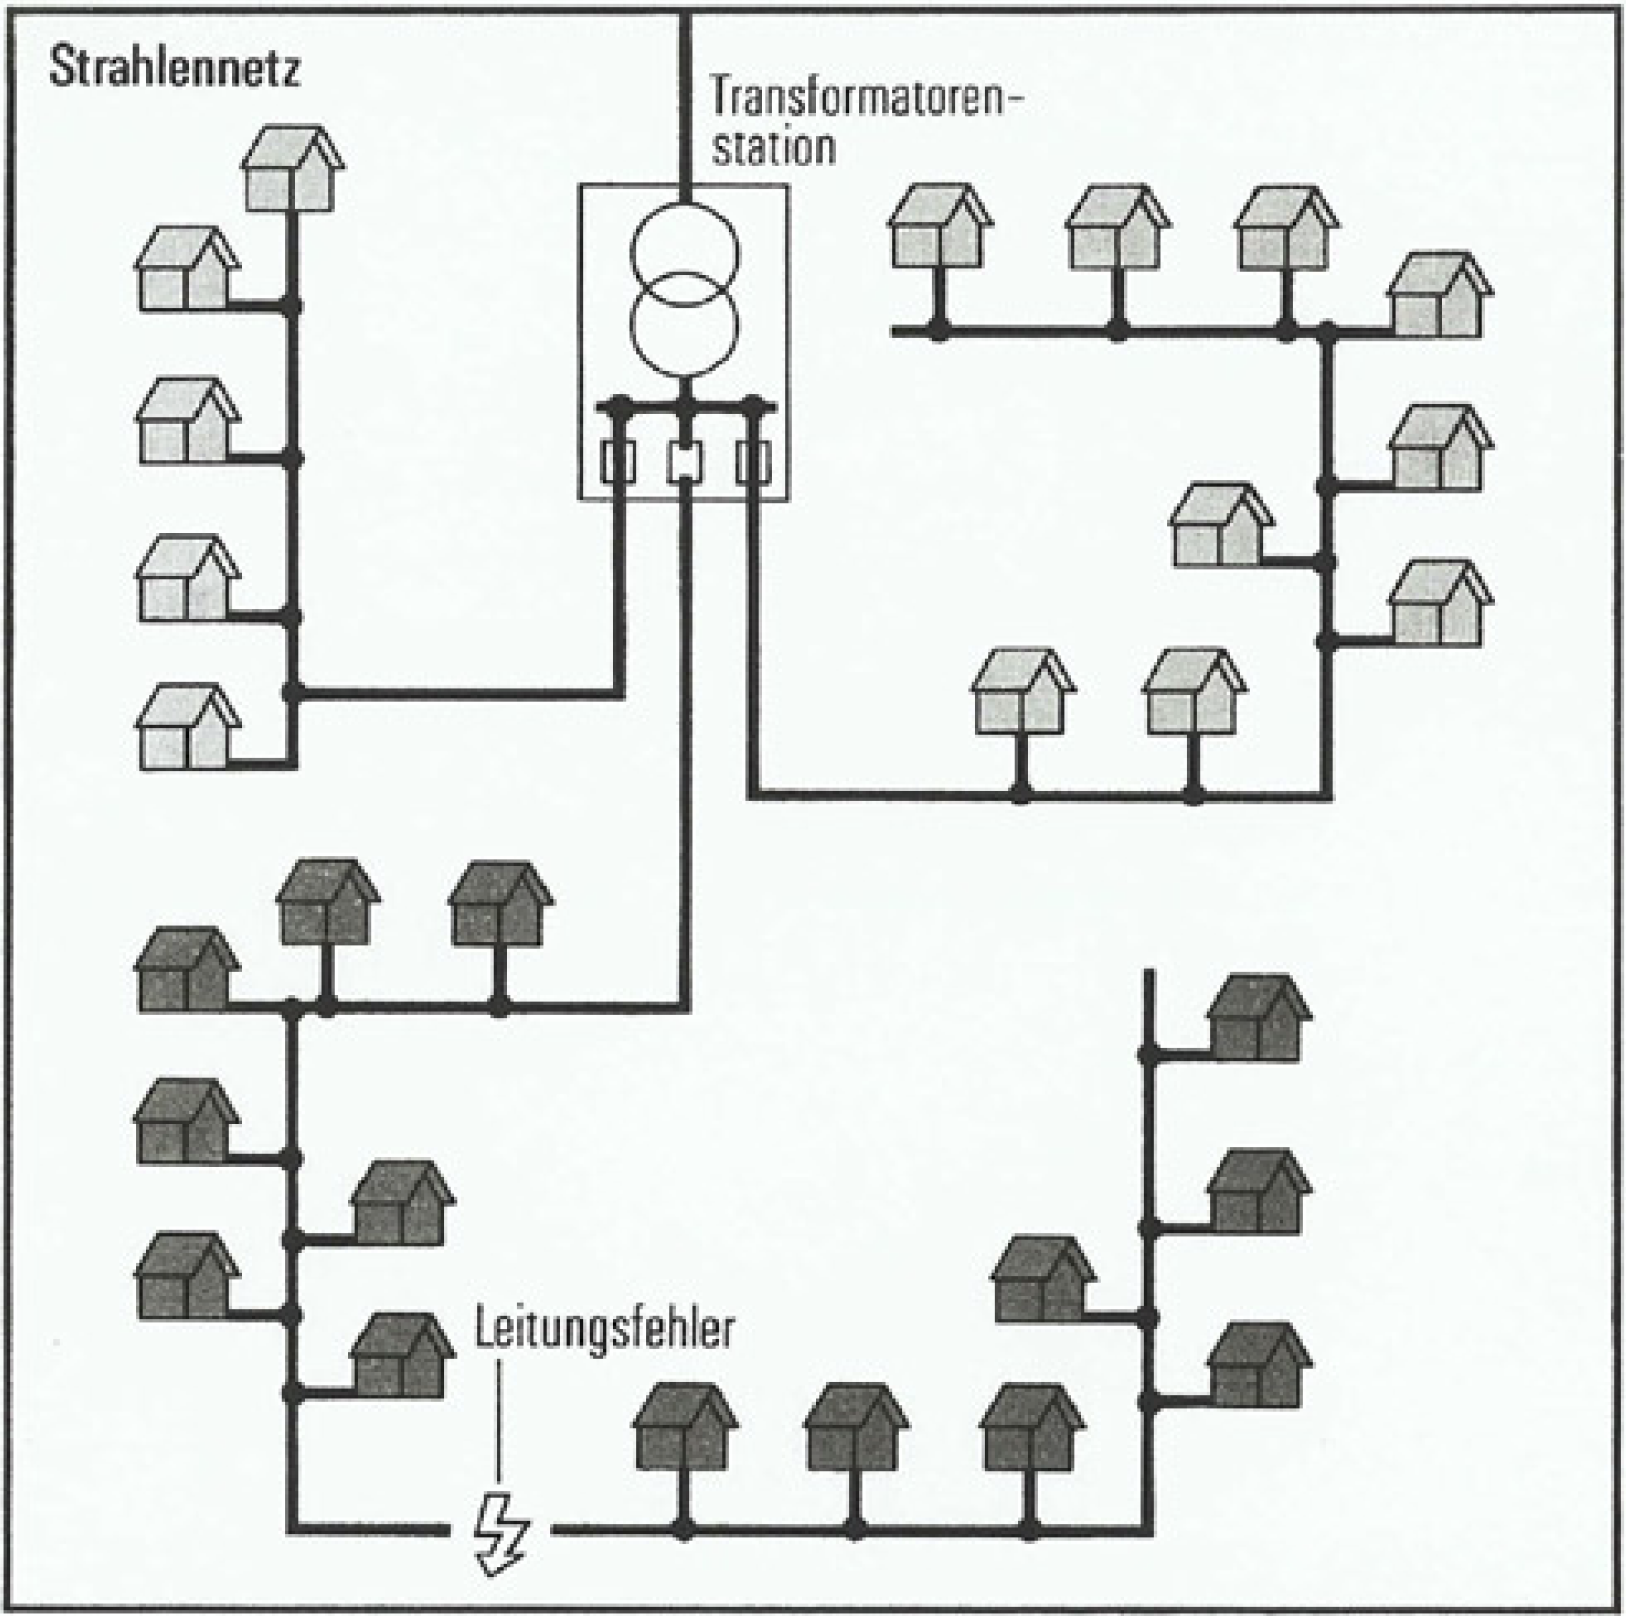
\includegraphics[width=0.55\columnwidth, align=c]{images/Strahlnetz.png}

\textbf{Pro:}
    \begin{itemize}
        \item geringer Planungsaufwand
        \item große Übersichtlichkeit bei der Fehlersuche
        \item geringe Anforderungen an den Netzschutz
    \end{itemize}
\vspace{1em}
\textbf{Contra:}
    \begin{itemize}
        \item größer werdende Spannungsabfälle mit zunehmendem Abstand von der Einspeisung
        \item höhere Leistungsverluste mit zunehmendem Abstand von der Einspeisung
    \end{itemize}


\subsection{Ringnetz}

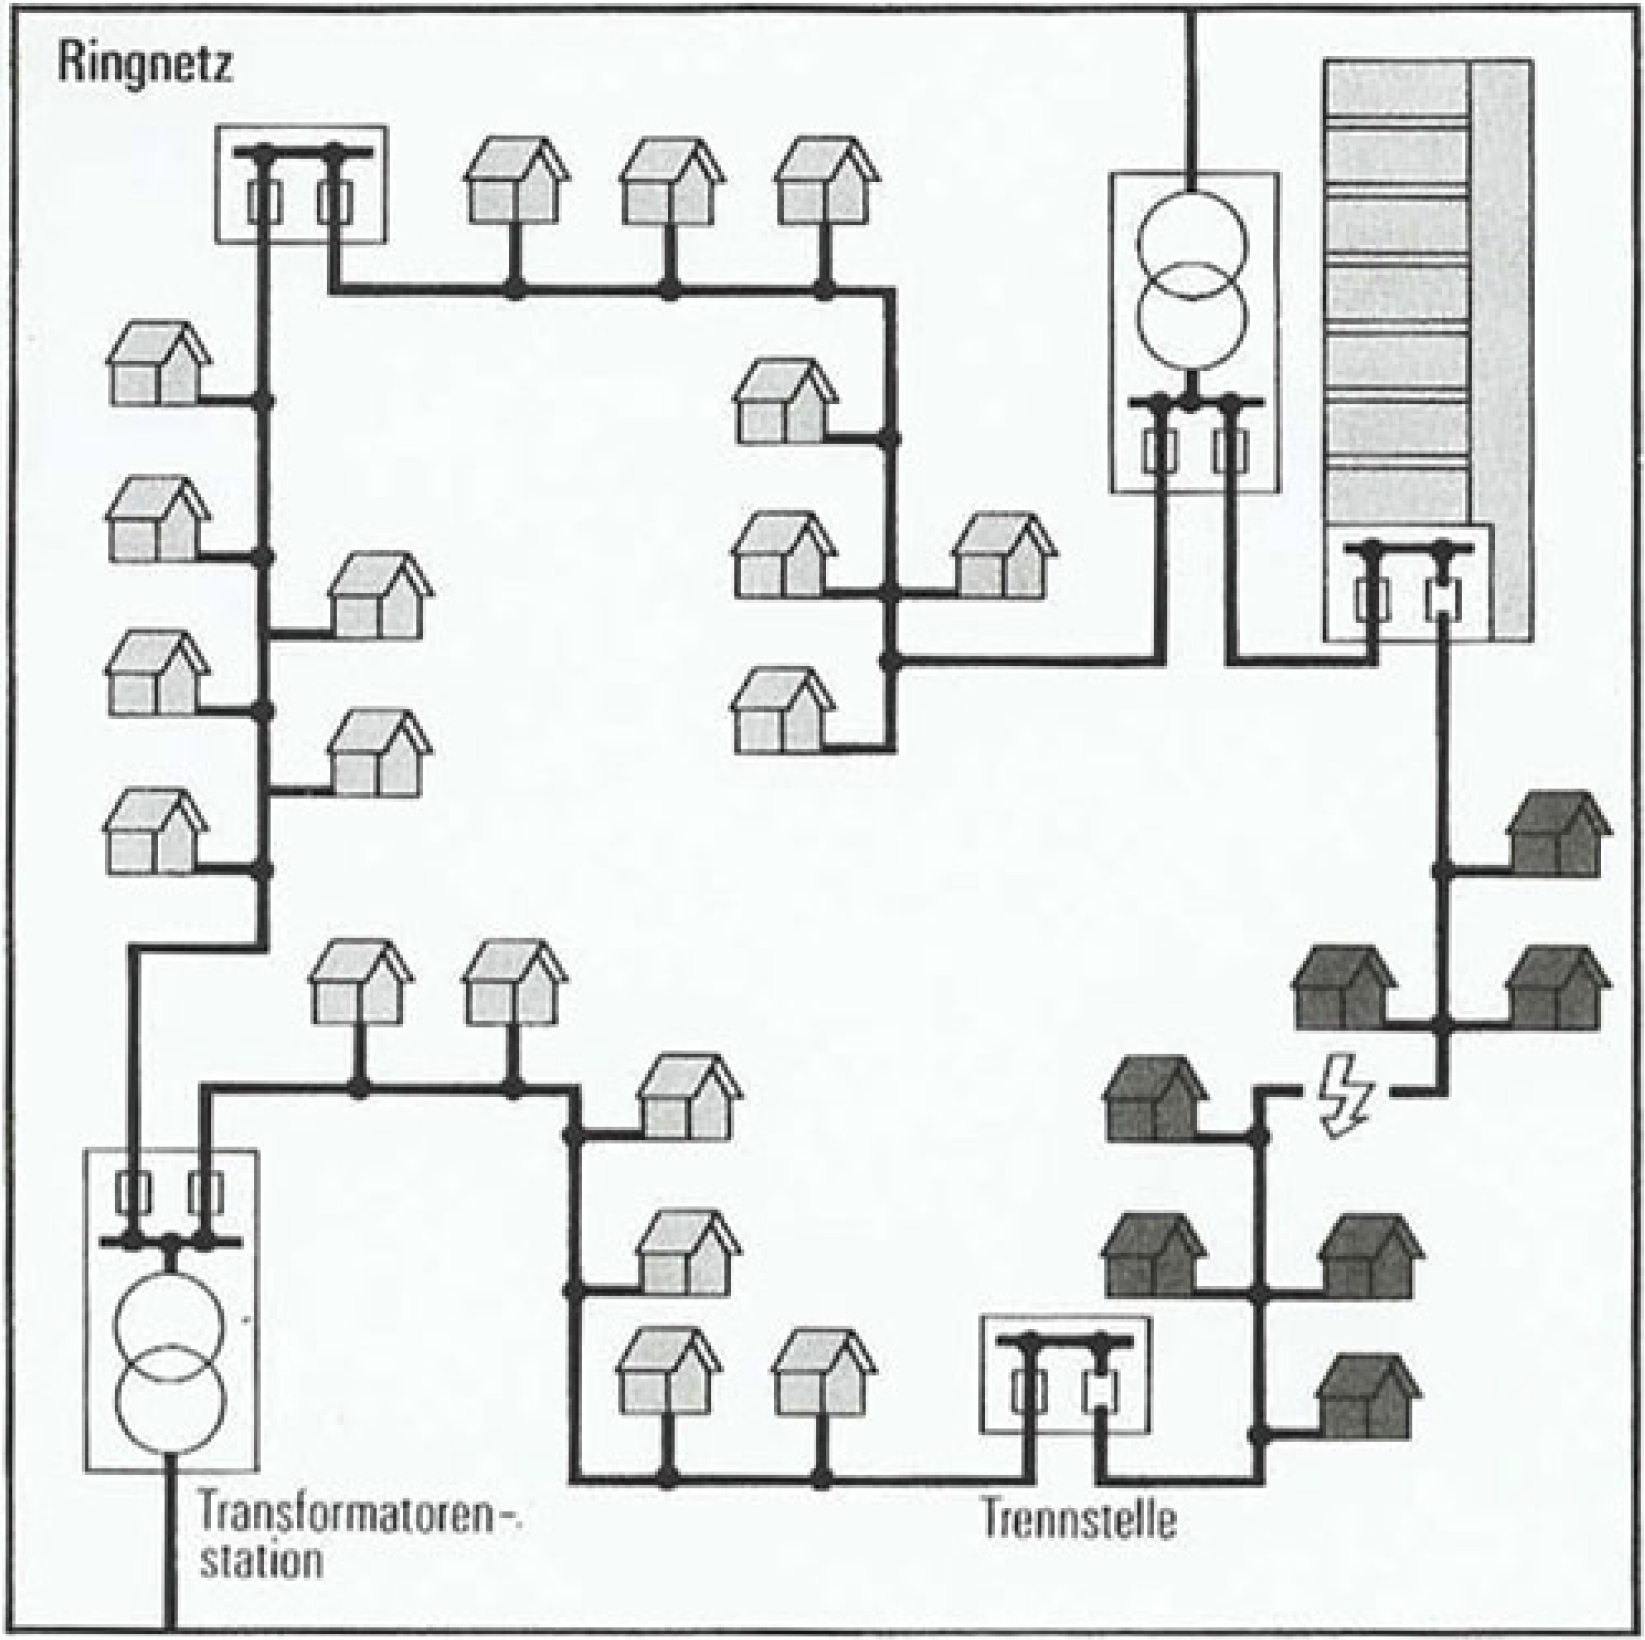
\includegraphics[width=0.55\columnwidth, align=c]{images/Ringnetz.png}

\textbf{Pro:}
\begin{itemize}
    \item höhere Versorgungssicherheit
    \item geringere Verluste
    \item verbesserte Spannungshaltung
\end{itemize}

\vspace{1em}
\textbf{Contra:}
\begin{itemize}
    \item höhere Anspruch an die Qualifikation des Wartungspersonals
\end{itemize}

\subsection{Maschennetz}

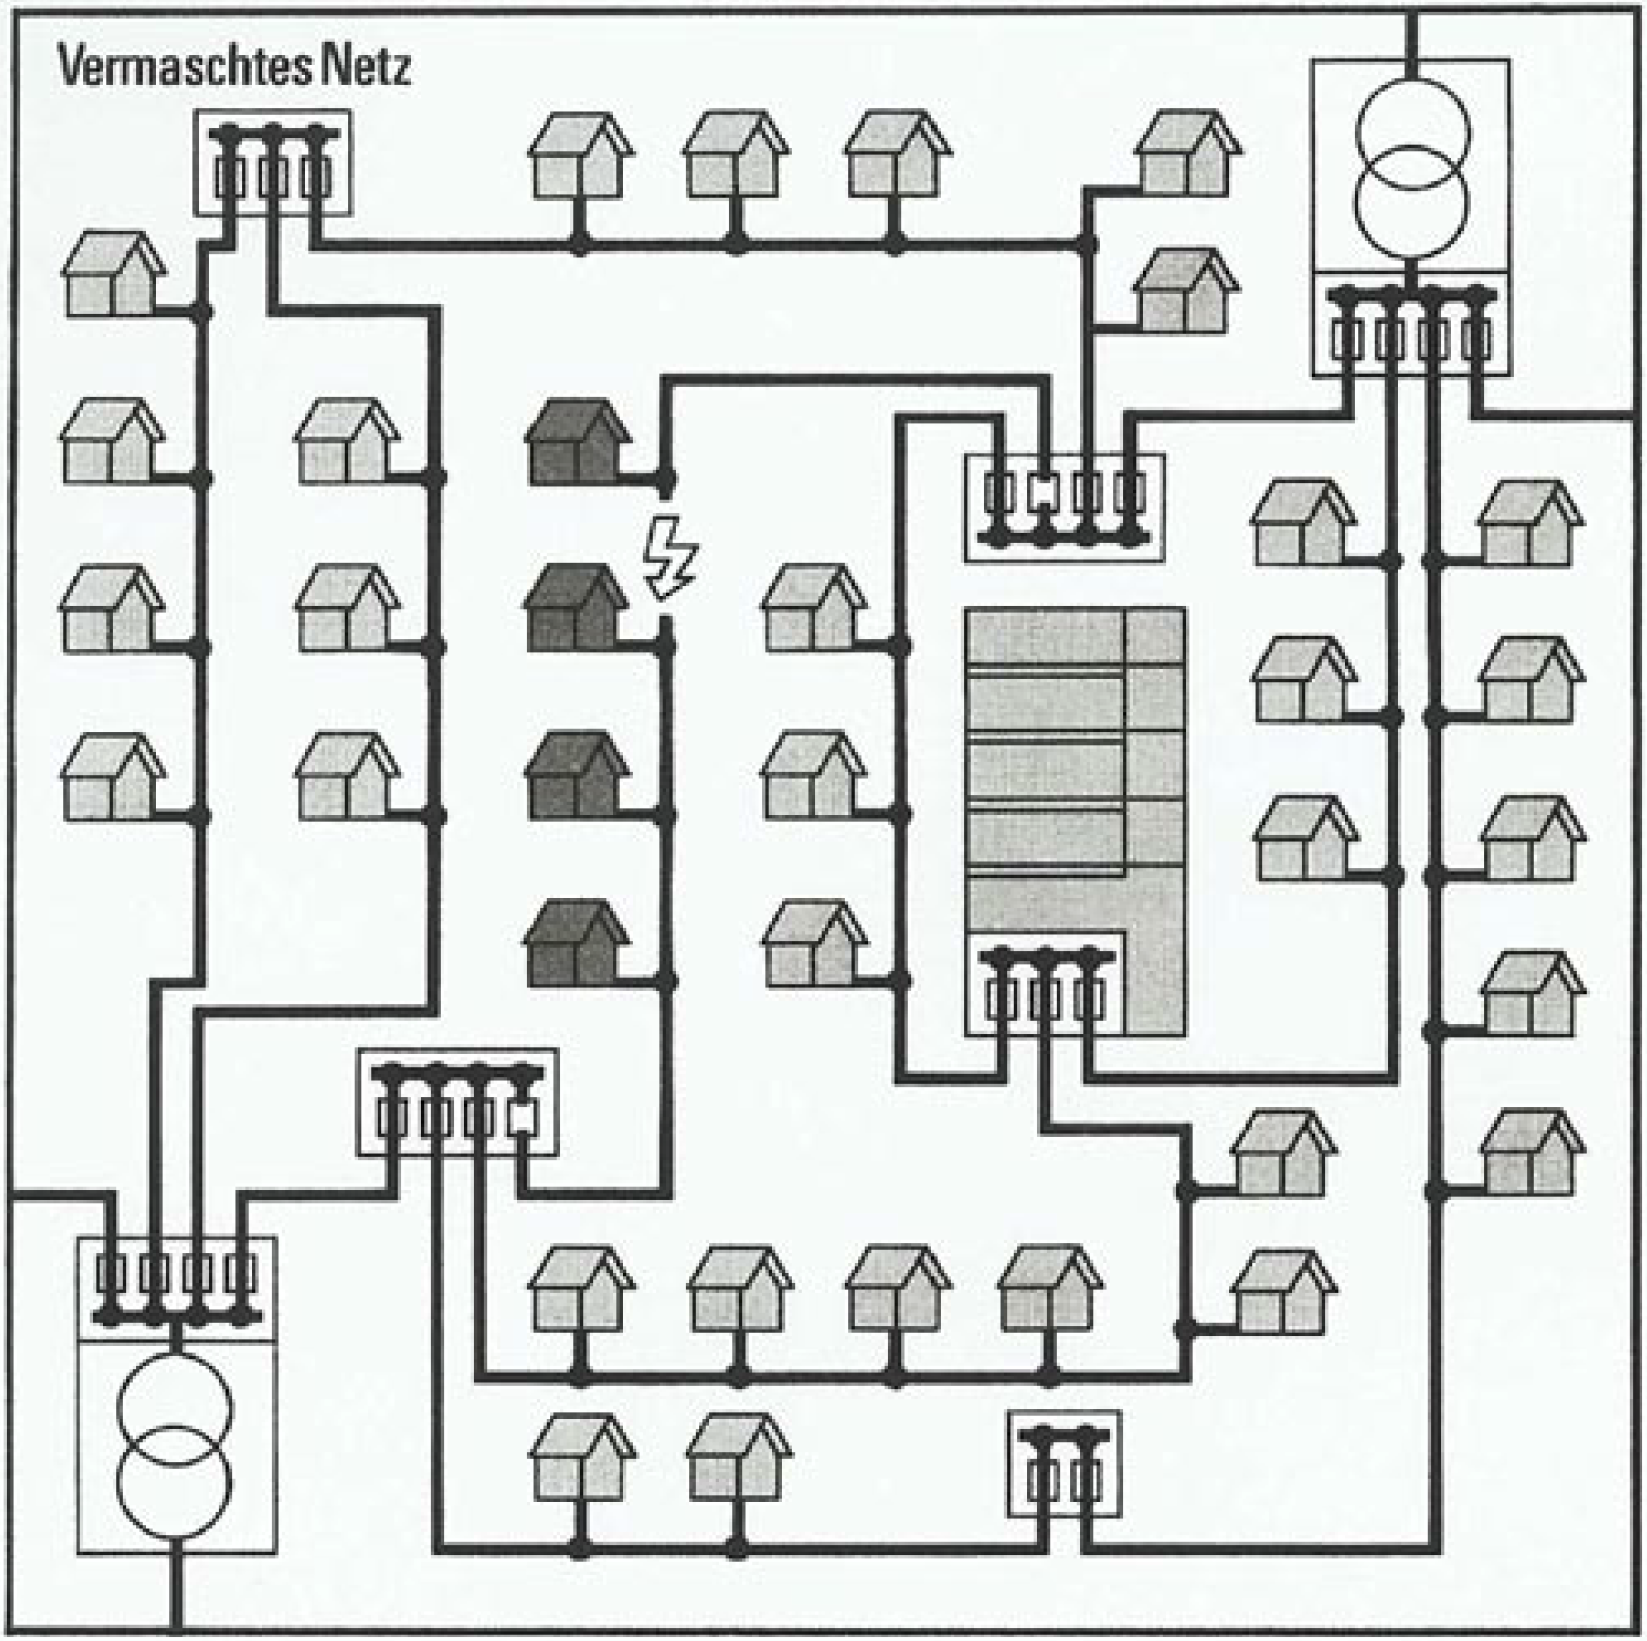
\includegraphics[width=0.55\columnwidth, align=c]{images/Maschennetz.png}

\textbf{Pro:}
\begin{itemize}
    \item eine optimale Versorgungszuverlässigkeit
    \item optimale Spannungshaltung
    \item minimale Leistungsverluste
\end{itemize}

\vspace{1em}
\textbf{Contra:}
\begin{itemize}
    \item hohe Investitionskosten
    \item hohe Projektions- und Wartungsaufwand
    \item höhere Kurzschlussströme
\end{itemize}














        %\section{Leitungen}

\textbf{Aufgabe:}
\begin{itemize}
    \item  Energieübertragung und -verteilung\\
\end{itemize}

\textbf{Wichtigsten Leitungsarten:}
\begin{itemize}
    \item Freileitung
    \item Kabelleitung
    \item \textbf{Freileitungen} in praktisch allen Spannungsebenen von der Niederspannung bis zur Höchstspannung.
    \item \textbf{Kabelleitungen} mehr in den unteren Spannungsebenen.
\end{itemize}


\subsection{Freileitungen}

\begin{itemize}
    \item \textbf{Material:}
    \begin{itemize}
        \item Al-Seile (99{,}5\% Al), Aldrey-Seile (> 98{,}5\% Al, Mg, Si, Fe) und Al-Stahl-Seile\\ 
        (Verhältnis Alu:Stahl typ. 6:1, z.\,B. 240/40 mm\textsuperscript{2}), Kupfer ist bei neuen Leitungen immer seltener
        \item Aluminium-Drähten $\Rightarrow$ eine gute elektrische Leitfähigkeit
        \item Stahlkern $\Rightarrow$ mechanische Festigkeit
        \item Aluminium hat gegenüber Kupfer einen deutlichen Preisvorteil
    \end{itemize}

    \item Ab 220\,kV $\Rightarrow$ Bündelleiter $\Rightarrow$ Sie führen also zur 
    \textbf{Verminderung des Wellenwiderstandes} und damit 
    \textbf{zur Erhöhung der übertragbaren Leistung.}

    \item \textbf{Hochtemperaturleiter:}
    \begin{itemize}
        \item normale Leiterseile $T_{\text{max}} = 80\,^{\circ}\mathrm{C}$
        \item Hochtemperaturseilen $T_{\text{max}} = 210\,^{\circ}\mathrm{C}$
        \item \textbf{Steigerung der Übertragungskapazität um bis zu 50 Prozent}
    \end{itemize}
\end{itemize}


\subsection{Masten}

\textbf{Funktionen:}
\begin{itemize}
    \item \textbf{Tragmast:} Tragwerke für die Aufhängung der Leiter einer Freileitung
    \item \textbf{Abspannmasten:} An Winkelpunkten nehmen sie die Zugkräfte der Leiterseile auf.
    \item \textbf{Verdrillmast:} alle Aussenleiter eines Stromkreises auf dem Mast tauschen ihre Plätze\\
    (verbessertes Übertragungsverhalten).
\end{itemize}

\vspace{1em}
\textbf{Materialien:}
\begin{itemize}
    \item Stahl-Gittermast
    \item Betonmast
    \item Stahlrohrmast
    \item Holzmast
\end{itemize}


\subsection{Unterscheidungsmerkmale Freileitungen}

\textbf{Die wichtigsten Unterscheidungsmerkmale:}

\begin{itemize}
    \item Anzahl Phasen
    \item Länge der Isolatorenketten (Je höher die Spannung, umso länger sind die Isolatorenketten)
    \item Abstand der Phasen und Höhe der Masten
\end{itemize}

\begin{minipage}[c]{0.48\columnwidth}
    \begin{center}
        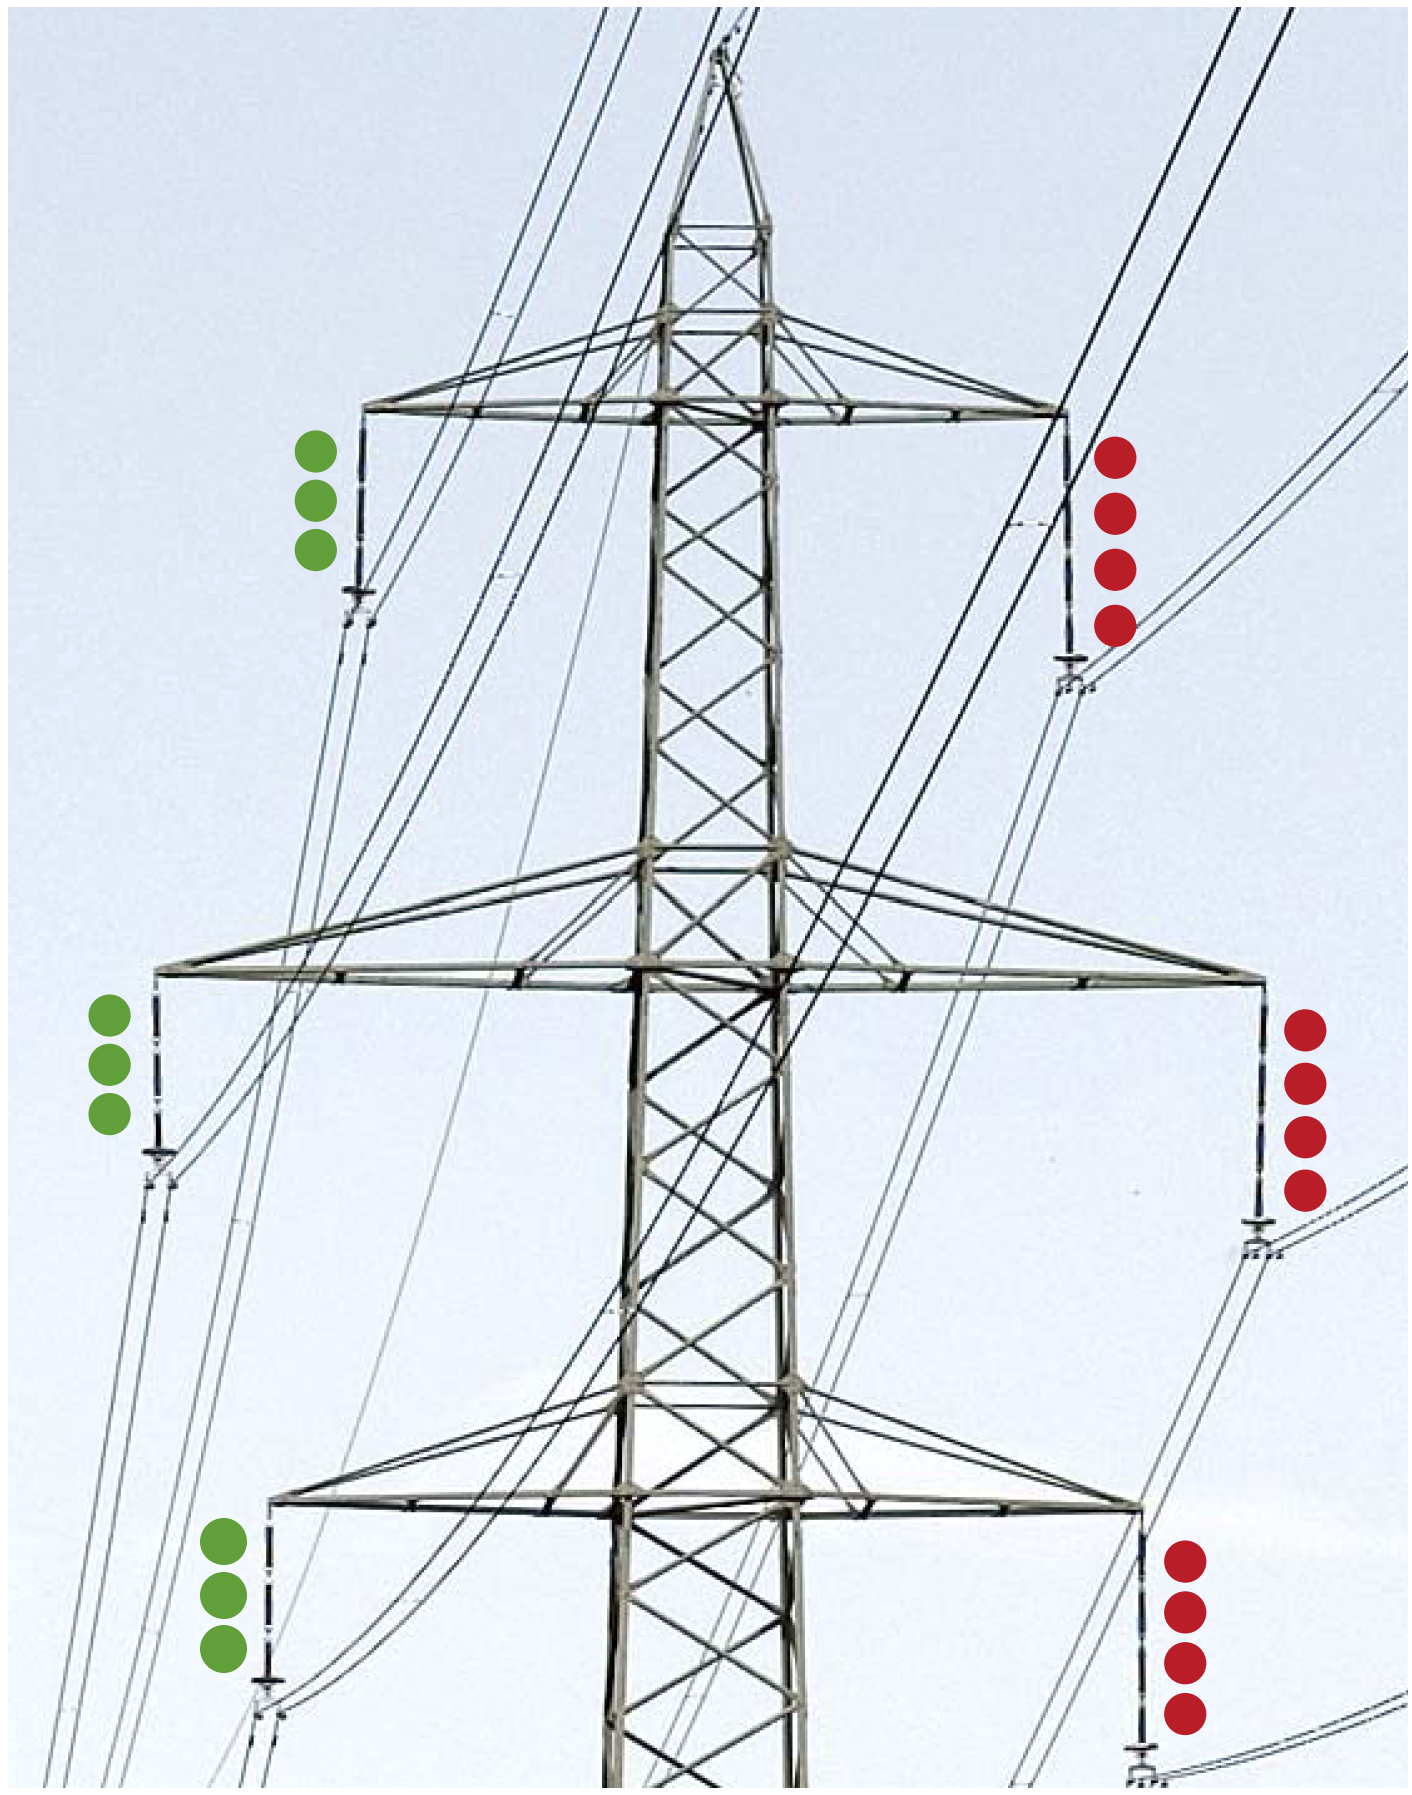
\includegraphics[width=0.9\textwidth, align=c]{images/Freileitungen_1.png}
    \end{center}
\end{minipage}
\hfill
\begin{minipage}[c]{0.48\columnwidth}
    \begin{center}
        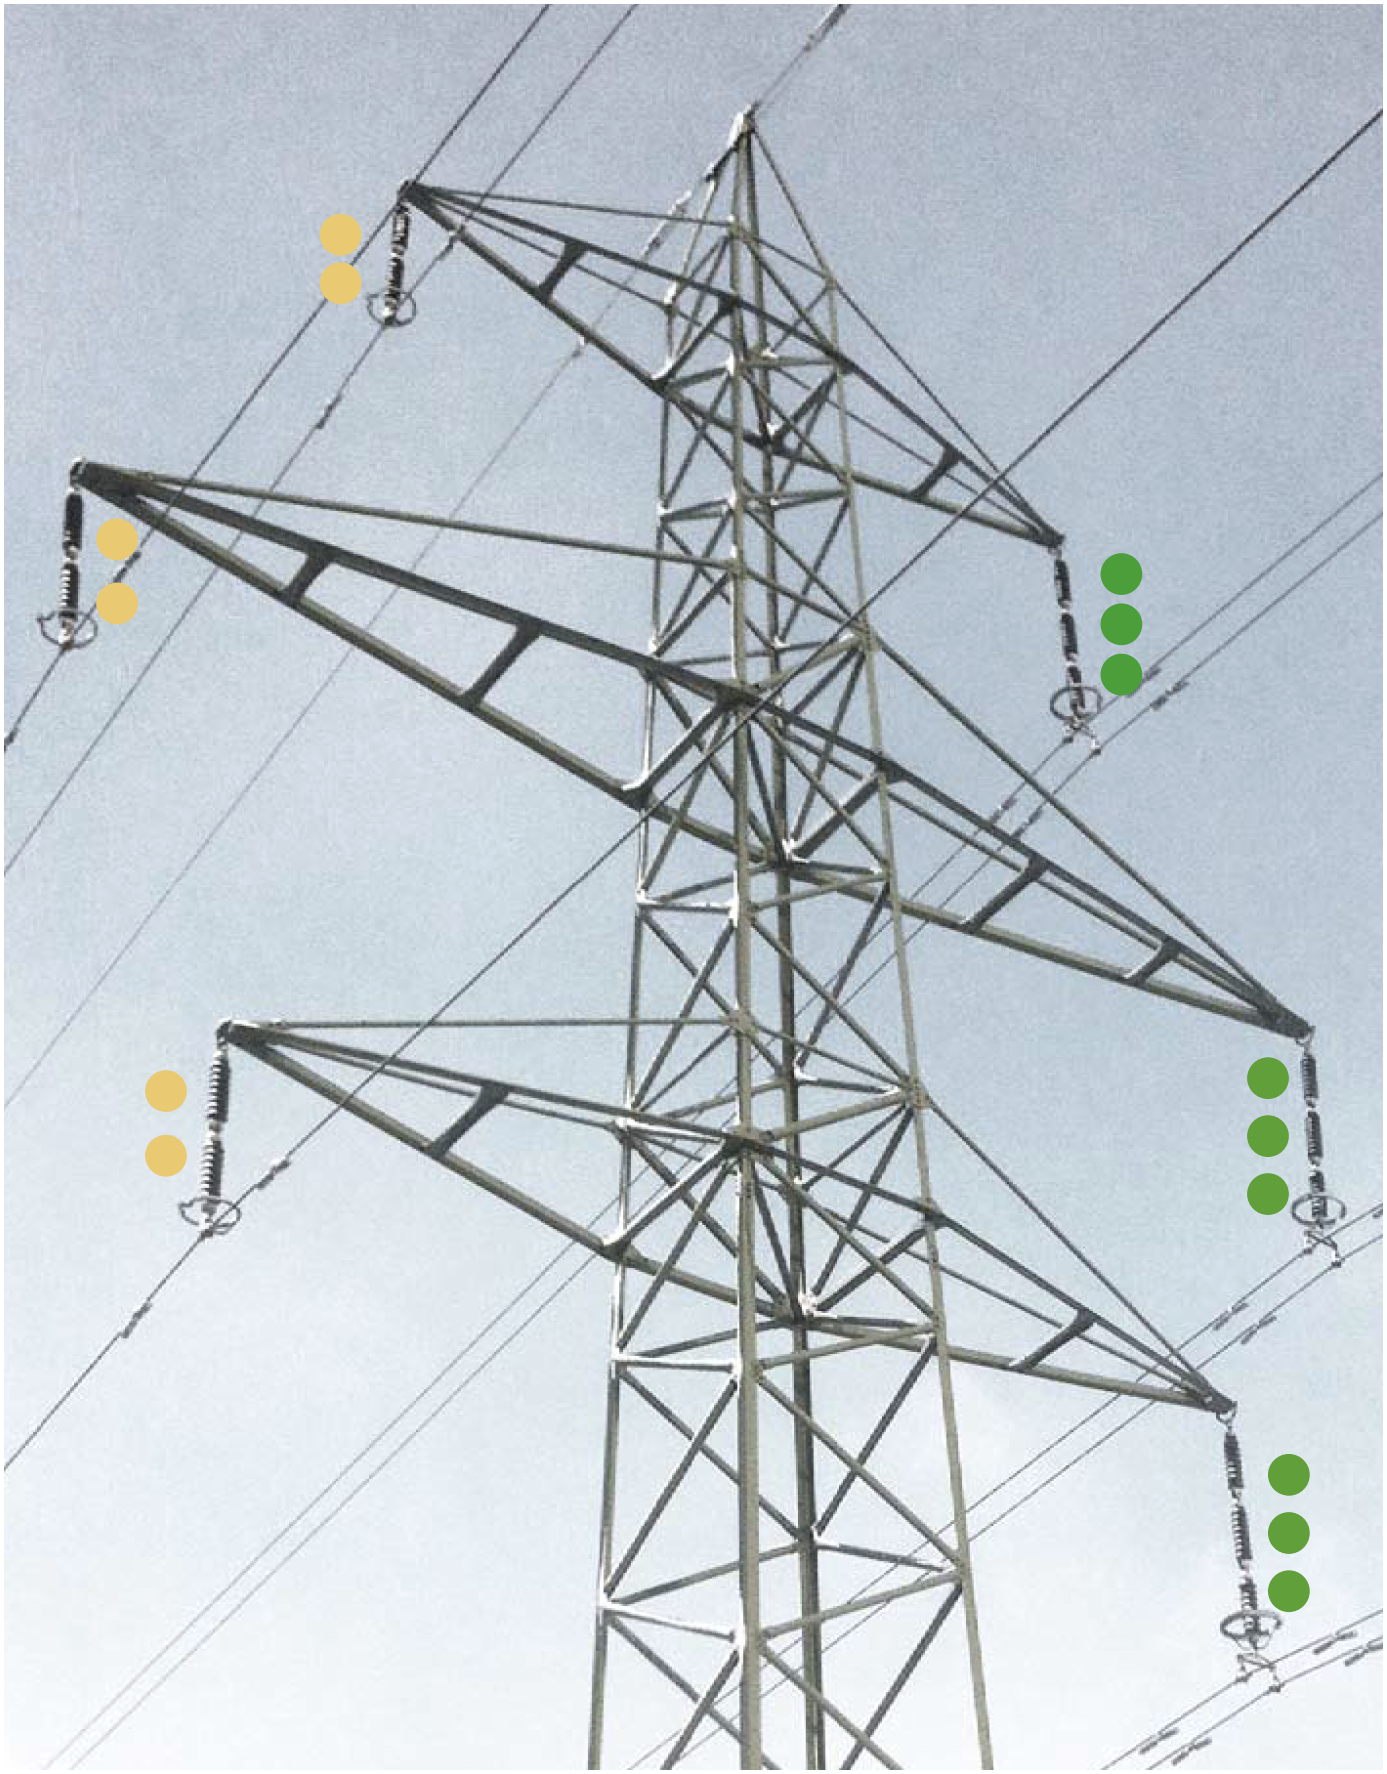
\includegraphics[width=0.9\textwidth, align=c]{images/Freileitungen_2.png}
    \end{center}
\end{minipage}

\subsection{Mastenformen}

\begin{minipage}[c]{0.4\columnwidth}
    \subsubsection{Donaumast}
\end{minipage}
\hfill
\begin{minipage}[c]{0.56\columnwidth}
    \subsubsection{Einebenenmast}
\end{minipage}

\begin{minipage}[c]{0.4\columnwidth}
    Zwei Drehstromkreise bei denen die Leiter jeweils im Dreieck angeordnet sind
\end{minipage}
\hfill
\begin{minipage}[c]{0.56\columnwidth}
    Niedrigen Bauhöhe und eine grössere Trassenbreite
\end{minipage}

\begin{minipage}[c]{0.4\columnwidth}
    \begin{center}
        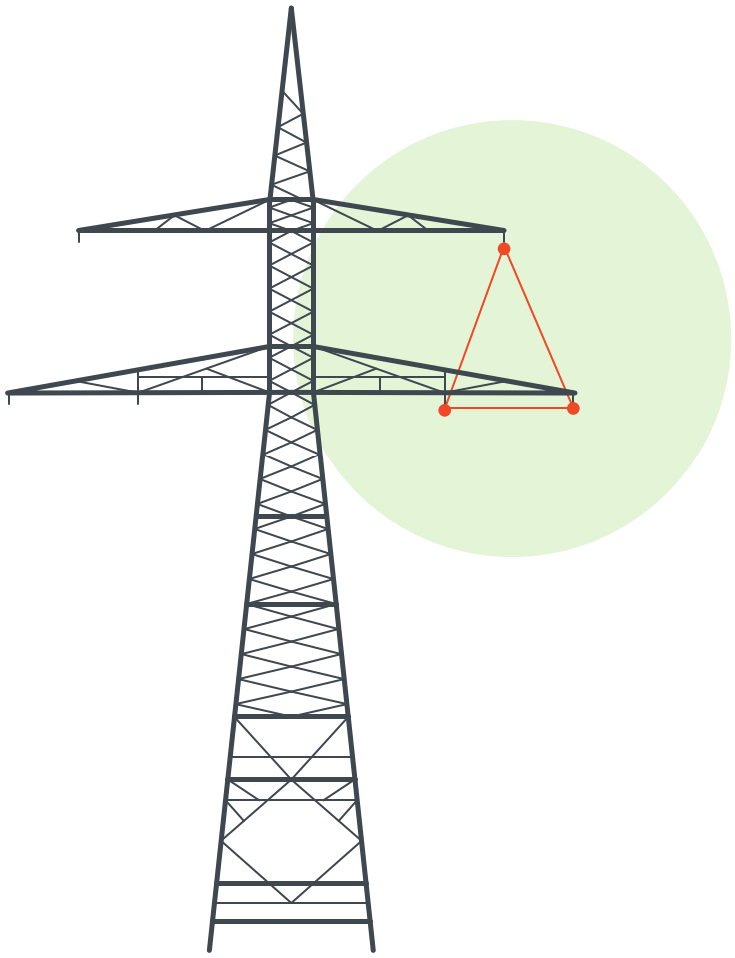
\includegraphics[height=5cm, align=c]{images/Mastenformen_1.png}
    \end{center}
\end{minipage}
\hfill
\begin{minipage}[c]{0.56\columnwidth}
    \begin{center}
        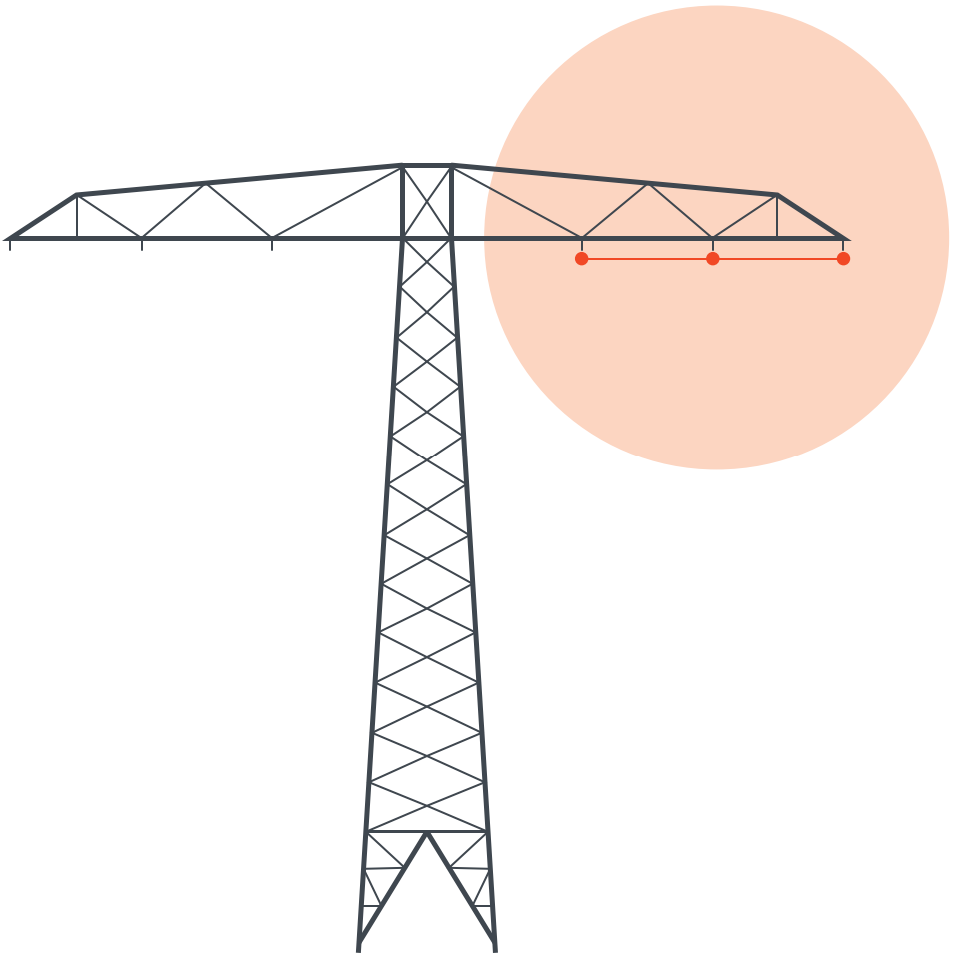
\includegraphics[height=5cm, align=c]{images/Mastenformen_2.png}
    \end{center}
\end{minipage}

\begin{minipage}[c]{0.5\columnwidth}
    \subsubsection{Tonnenmast}
    Eine geringe Trassenbreite, sind aber höher als vergleichbare Donaumasten

    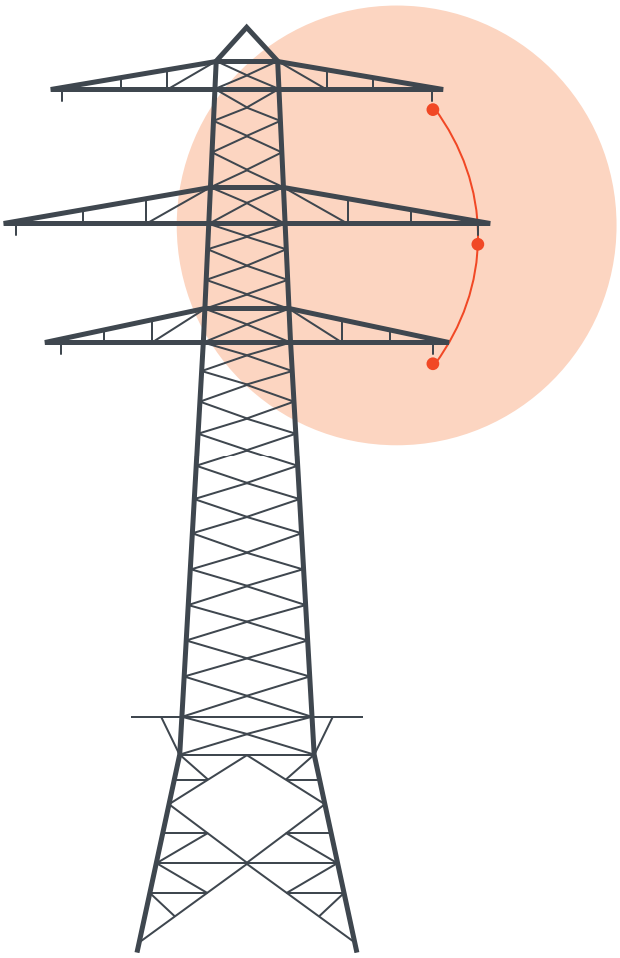
\includegraphics[height=5cm, align=c]{images/Mastenformen_3.png}    
\end{minipage}


\subsection{Freileitungen: Vor- und Nachteile}

\textbf{Pro:}
\begin{itemize}
    \item günstige Investitionskosten
    \item bessere Zugänglichkeit bei Reparaturen $\Rightarrow$ kürzere Wiederinbetriebnahmezeiten
\end{itemize}
\vspace{1em}
\textbf{Contra:}
\begin{itemize}
    \item atmosphärischen Einwirkungen ausgesetzt
    \item Akzeptanzprobleme
\end{itemize}


\section{Kabelleitungen}

\subsubsection{Material}

\begin{tabular}{>{\bfseries}l l}
    Leiter: & Kupfer oder Aluminium \\
    Isolierung: & öl-imprägniertes Papier oder Kunststoffe wie Polyäthylen (PE), \\
                & vernetztes Polyäthylen (VPE) sowie Polyvinylchlorid (PVC) \\
    Schutzmantel: & Metall \\
\end{tabular}


\subsection{Aufbau Allgemein}


\subsection{Aufbau}

\textbf{Gürtelkabel:}\\
Nichtradiales elektrisches Feld, Verwendung im Nieder- und Mittelspannungsbereich

\textbf{Dreimantel-Kabel:}\\
Radiales elektrisches Feld, Verwendung im Nieder- und Mittelspannungsbereich

\textbf{Einleiterkabel:}\\
Radiales elektrisches Feld, Verwendung im oberen Mittelspannungs- und im Hochpannungsbereich





\subsubsection{Kabel: Vor- und Nachteile}

\textbf{Pro:}
\begin{itemize}
    \item geschützt vor atmosphärischen Einwirkungen $\Rightarrow$ kleinere Ausfallsrate
    \item bessere Akzeptanz
\end{itemize}

\vspace{1em}
\textbf{Contra:}
\begin{itemize}
    \item schwierigere Zugänglichkeit bei Reparaturen $\Rightarrow$ längere Wiederinbetriebnahmezeiten
    \item im Hochspannungsbereich teurer (wirtschaftlich nur für kurze Strecken)
\end{itemize}


\subsection{Erdverkabelung in der Schweiz}

\textbf{Erdverkabelung pro Netzebene in der Schweiz}\\
\begin{tabular}{>{\bfseries}l r}
    Netzebene 1 & 8 km \\
    Netzebene 3 & 1'893 km \\
    Netzebene 5 & 30'607 km \\
    Netzebene 7 & 72'852 km \\
\end{tabular}




















        %\newpage
\section{Schaltanlagen / Umspannwerke}

\subsection{Aufgabe}

\begin{itemize}
    \item Stromfluss herstellen oder unterbrechen
    \item Betriebsmittel unter Spannung setzen oder spannungslos schalten
    \item Topologie ändern
    \item Strom- und Spannungsmessung
\end{itemize}

\subsection{Aufbau}

\begin{center}
    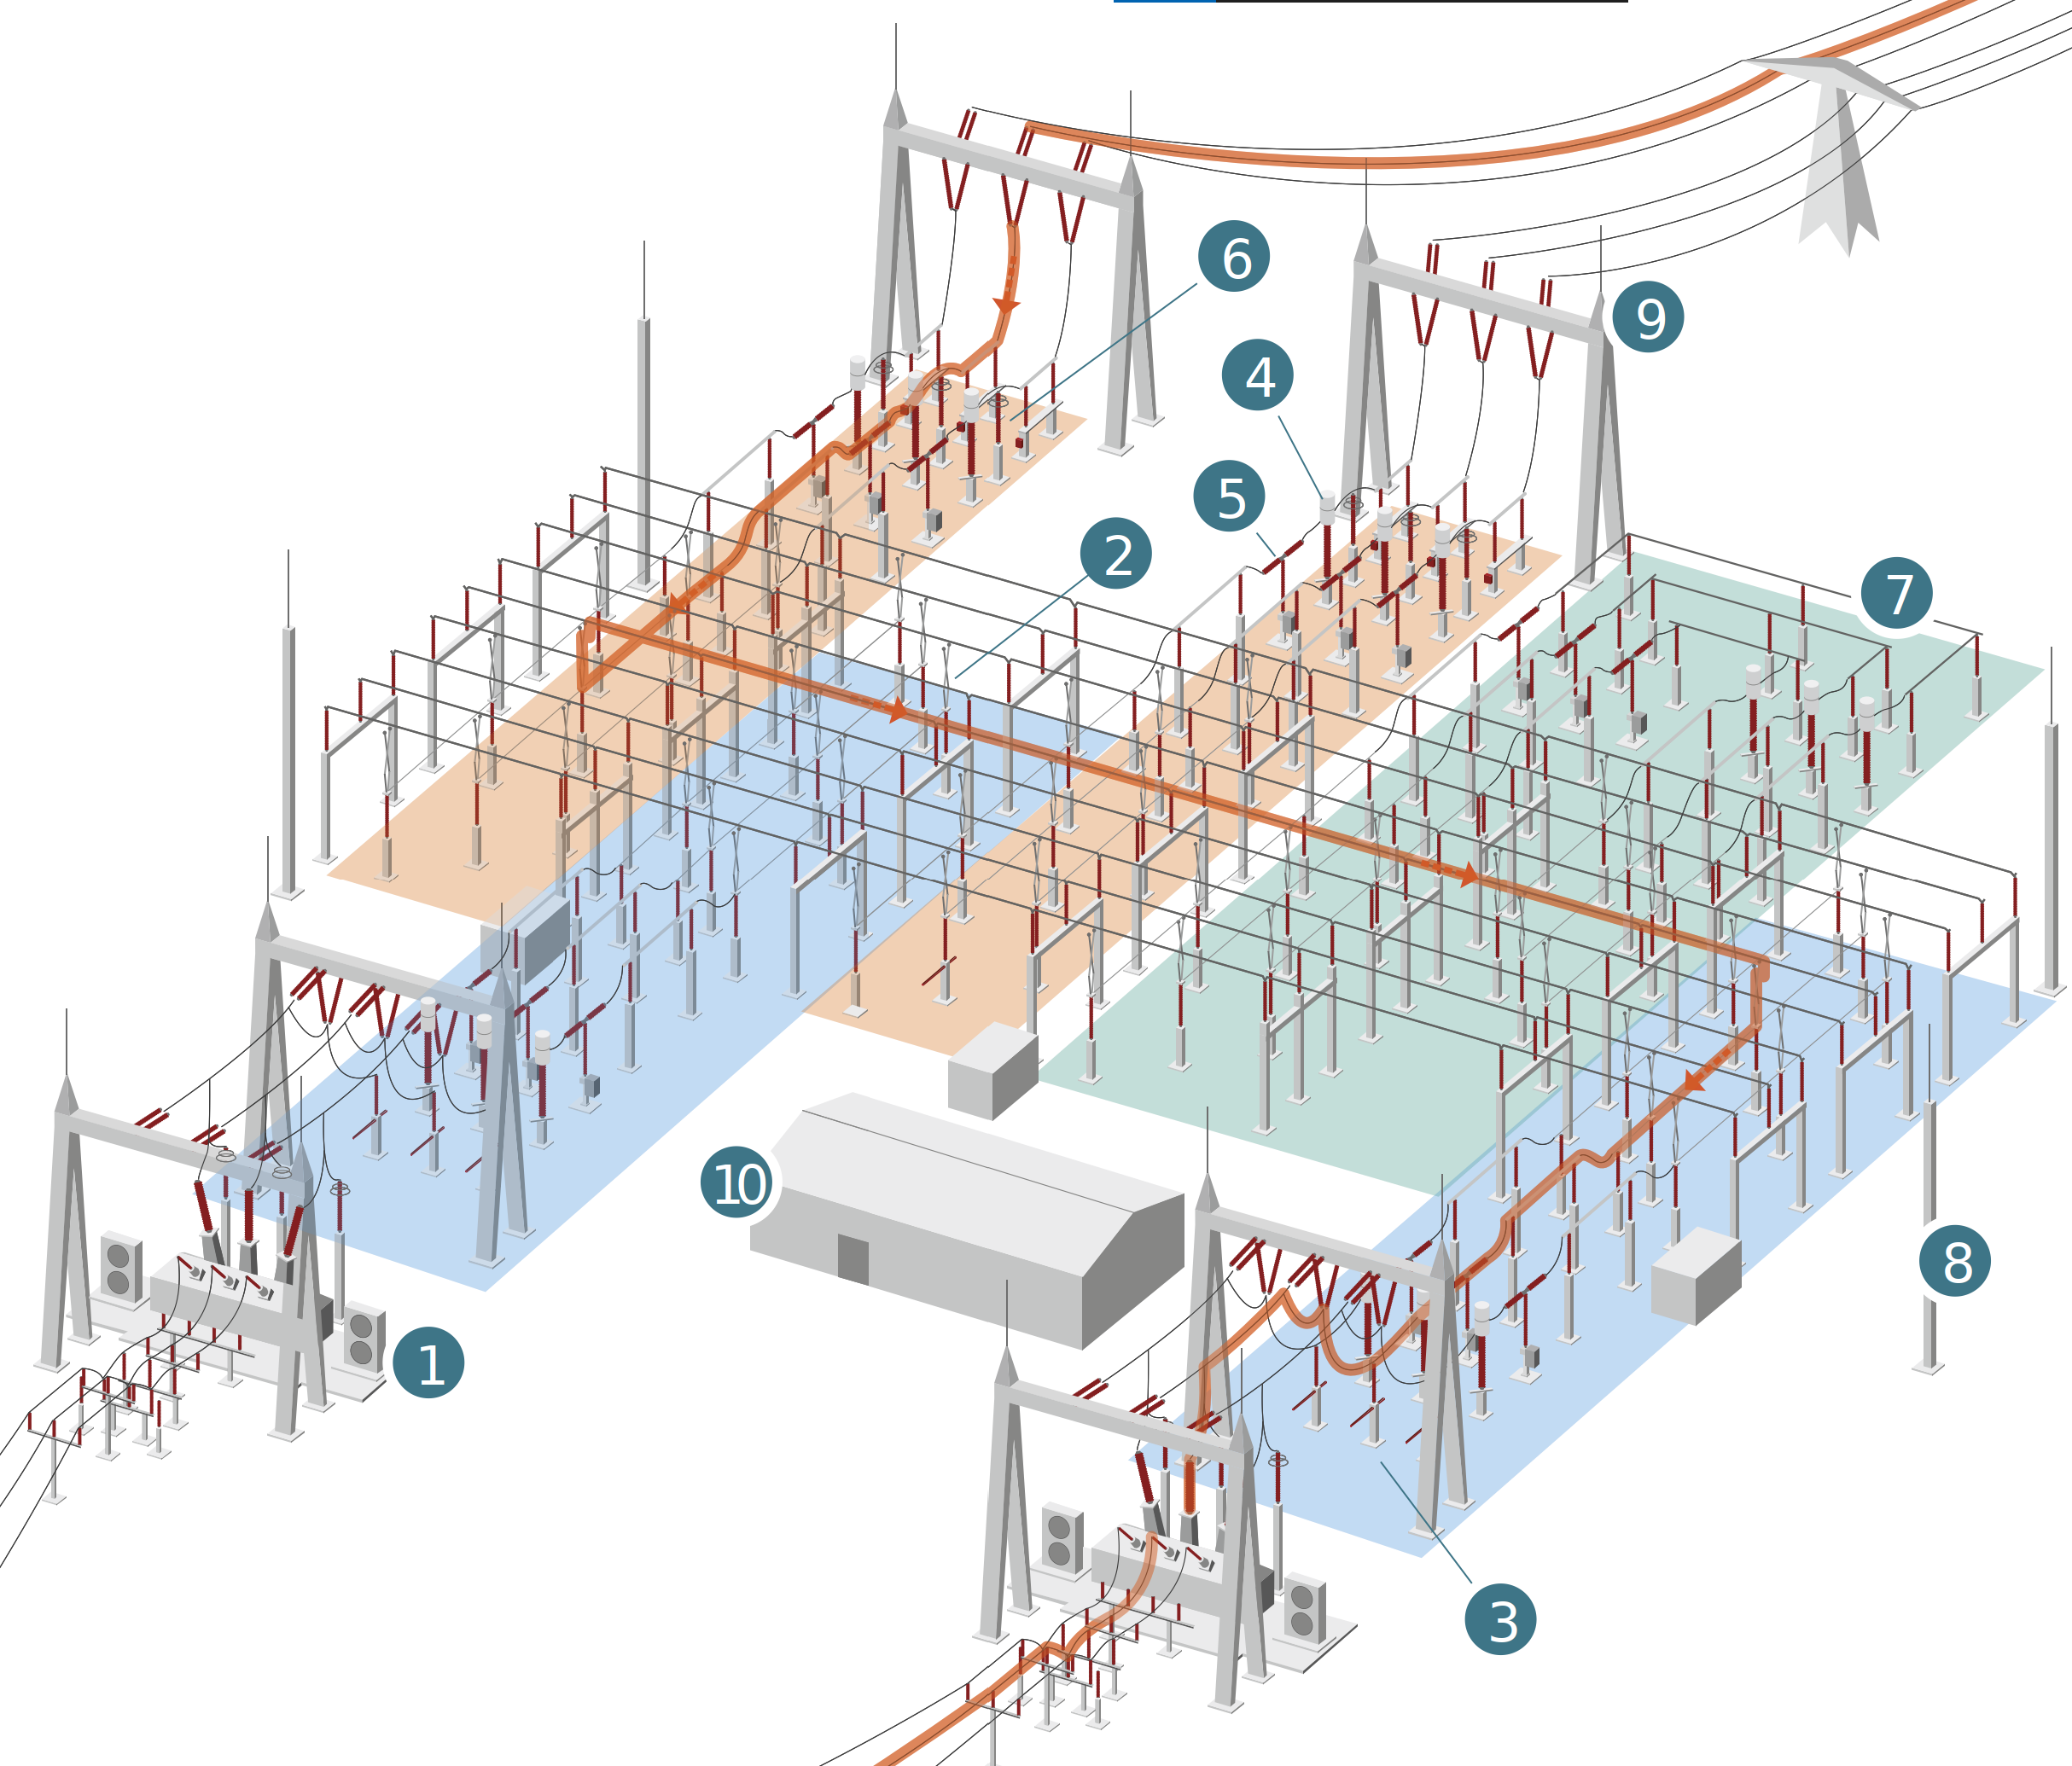
\includegraphics[width=0.98\columnwidth]{images/Aufbau_Schaltanlagen_1.png}
\end{center}

\begin{enumerate}
    \item Transformatoren
    \item Trennschalter
    \item Erdungsschalter
    \item Strom- und Spannungswandler
    \item Leistungsschalter
    \item Überspannungsableiter
    \item Sammelschiene
    \item Blitzschutzmast
    \item Portal
    \item Relais- und Betriebsgebäude
\end{enumerate}


\subsection{Transformator}

\begin{itemize}
    \item Veränderung der Spannung
    \item Öl zur Isolation und zum Wärmeabtransport
\end{itemize}

\begin{minipage}[c]{0.58\columnwidth}
    \begin{center}
        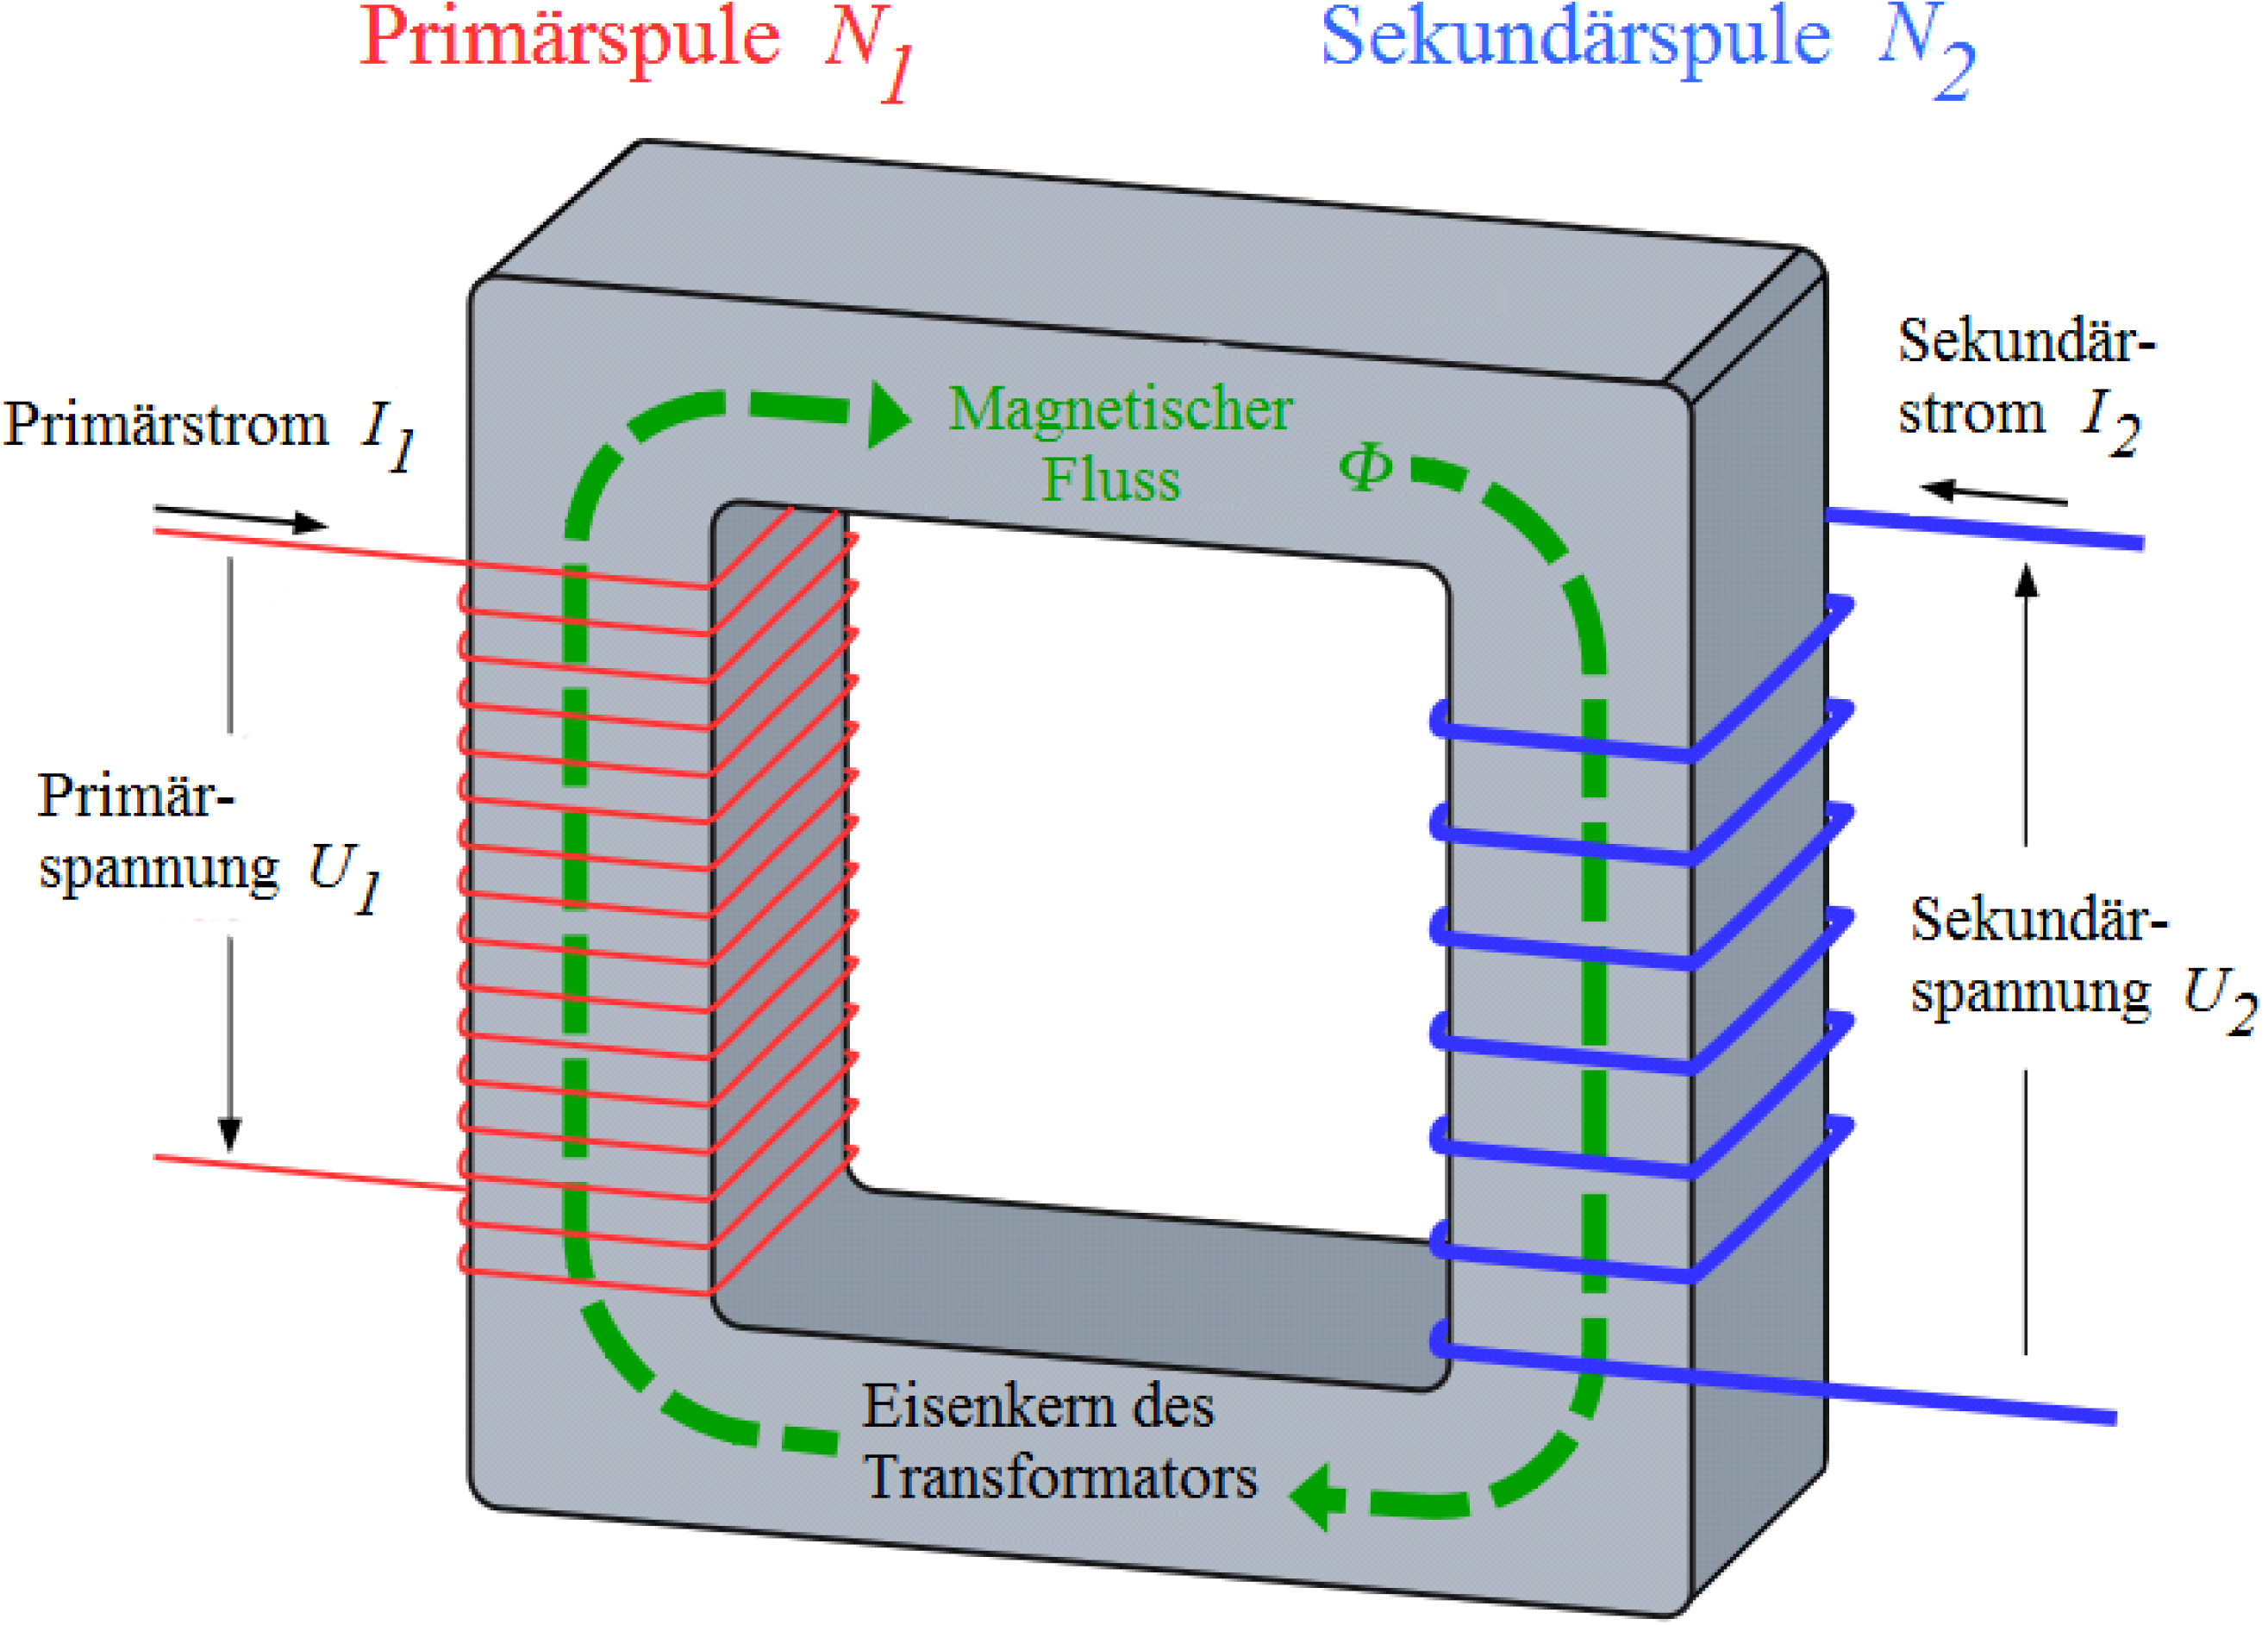
\includegraphics[width=0.98\textwidth, align=c]{images/Transformator_1.png}
    \end{center}
\end{minipage}
\hfill
\begin{minipage}[c]{0.38\columnwidth}
    \begin{center}
        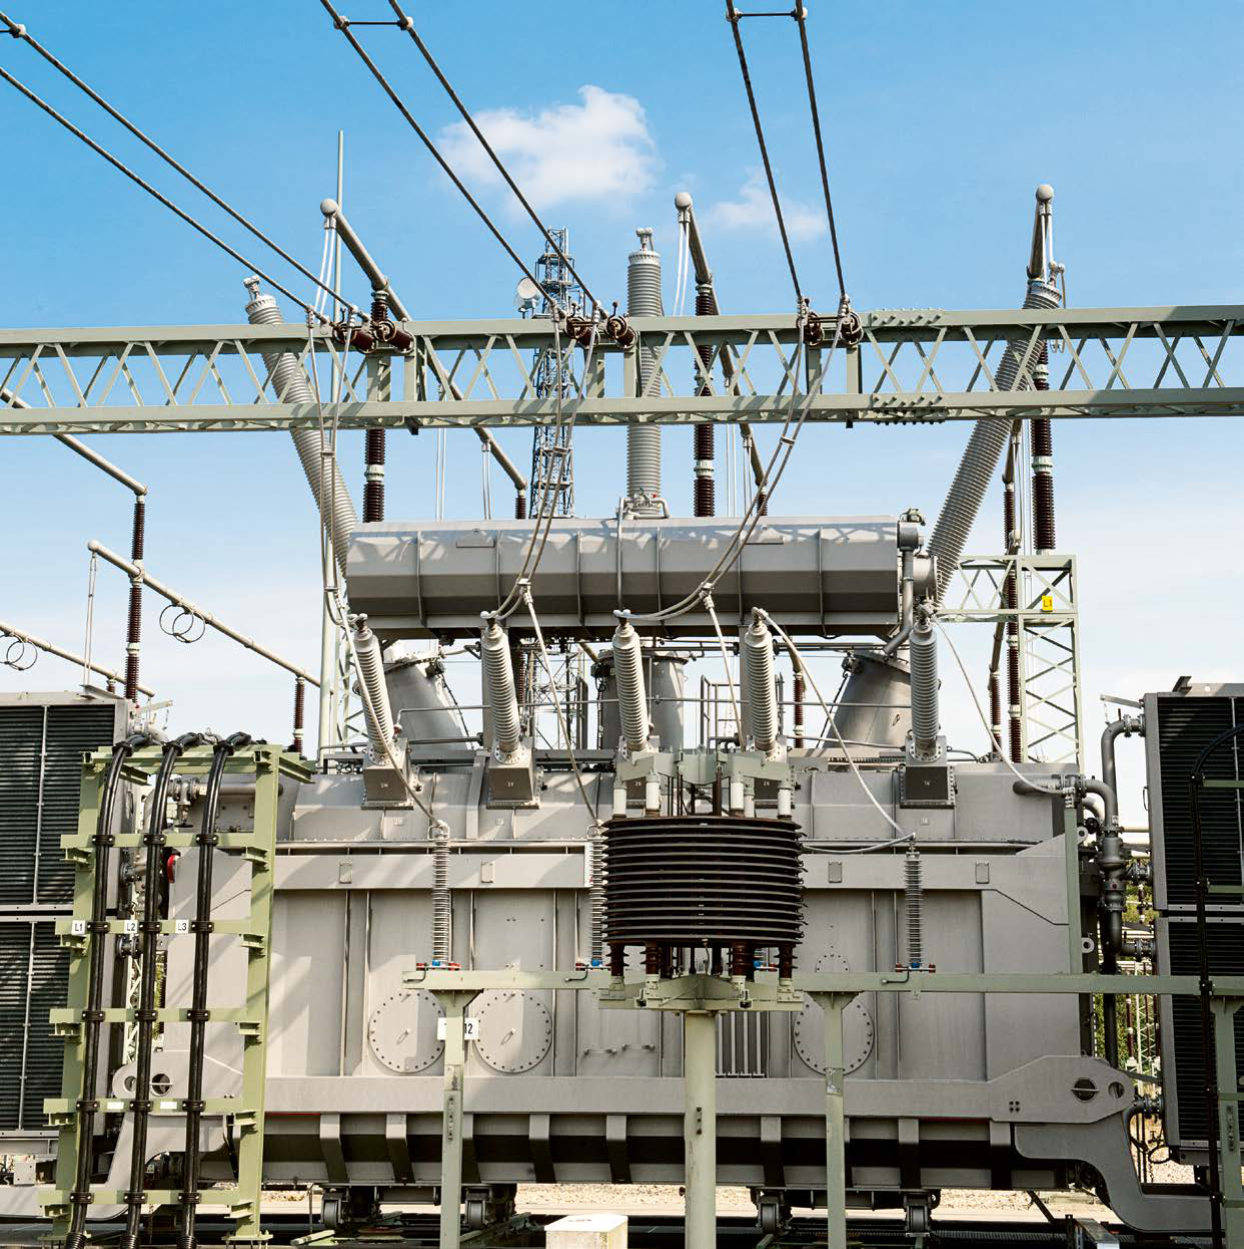
\includegraphics[width=0.98\textwidth, align=c]{images/Transformator_2.png}
    \end{center}
\end{minipage}


\subsection{Leistungsschalter}



\begin{minipage}[c]{0.28\columnwidth}
    \begin{center}
        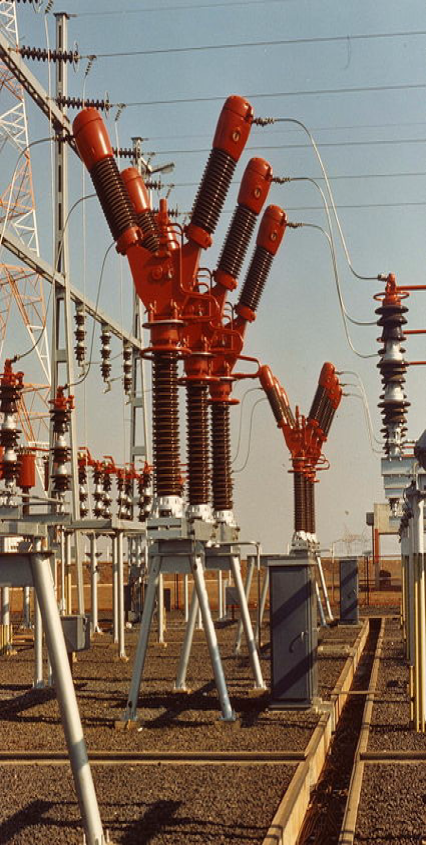
\includegraphics[width=0.98\textwidth, align=c]{images/Leistungsschalter.png}
    \end{center}
    
\end{minipage}
\hfill
\begin{minipage}[t]{0.68\columnwidth}
    \begin{itemize}
        \item Schaltet \textbf{Strom}
        \item Ein- und Ausschalten von Leitungen und Anlagenteile
        \item Schaltet im Normalbetrieb und im Fehlerfall\\(Kurzschlussstromunterbrechung)
    \end{itemize}
\end{minipage}


\subsection{Lastschalter}

\begin{itemize}
    \item Schaltet \textbf{Strom}
    \item Kann bis zu ca. 2-fachem Laststrom unterbrechen
\end{itemize}


\subsection{Trennschalter}

\begin{minipage}[c]{0.5\columnwidth}
    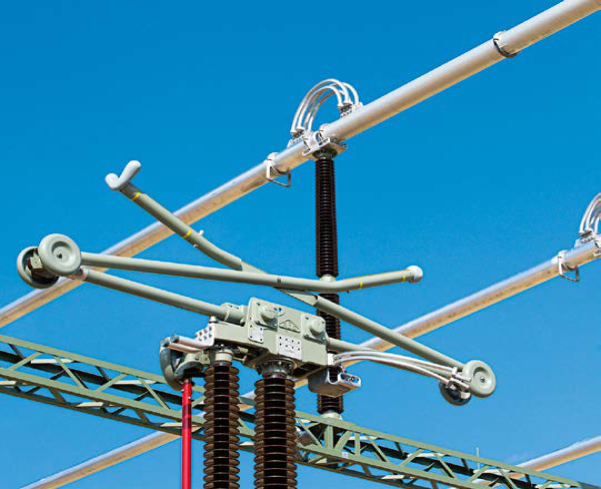
\includegraphics[width=0.98\textwidth]{images/Trennschalter.png}    
\end{minipage}

\begin{itemize}
    \item Leitungs- oder Sammelschienentrennschalter
    \item öffnen eines Stromkreises (Trennung einer Anlage von den restlichen Anlagen)
    \item Die Trennschalter schalten \textbf{keinen Strom}.
\end{itemize}


\subsection{Sonstiges}

\begin{minipage}[c]{0.48\columnwidth}
    \subsubsection{Messwandler}
\end{minipage}
\hfill
\begin{minipage}[c]{0.48\columnwidth}
    \subsubsection{Überspannungsableiter}
\end{minipage}

\begin{minipage}[c]{0.48\columnwidth}
    Messung der Spannung und Strom für Erkennung des Betriebszustandes
\end{minipage}
\hfill
\begin{minipage}[c]{0.48\columnwidth}
    Spannungsabhängiger Widerstand, Bei hoher Spannung verringert sich Widerstand schlagartig
\end{minipage}

\vspace{0.15cm}

\begin{minipage}[c]{0.48\columnwidth}
    \begin{center}
        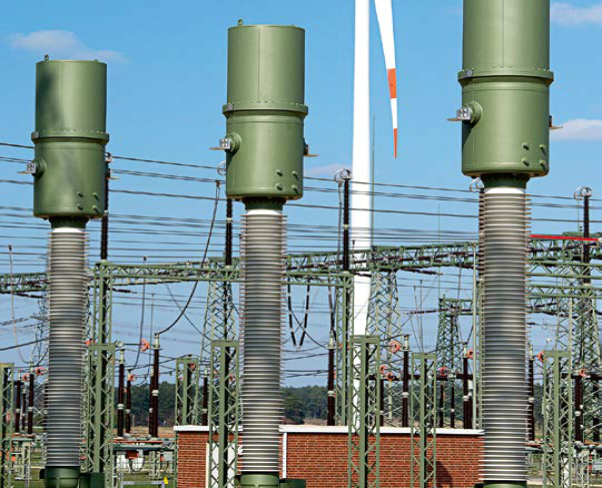
\includegraphics[width=0.98\columnwidth]{images/Messwandler.png}
    \end{center}
\end{minipage}
\hfill
\begin{minipage}[c]{0.48\columnwidth}
    \begin{center}
        \includegraphics[width=0.98\columnwidth]{images/Überspannungsableiter.png}
    \end{center}
\end{minipage}


\subsection{Schaltfelder Aufbau}

\begin{minipage}[c]{0.48\columnwidth}
    \subsubsection{Einfachsammelschiene}
\end{minipage}
\hfill
\begin{minipage}[c]{0.48\columnwidth}
    \subsubsection{Doppelsammelschiene}
\end{minipage}

\begin{minipage}[c]{0.48\columnwidth}
    \begin{itemize}
        \item übersichtliche und billige Lösung
    \end{itemize}
\end{minipage}
\hfill
\begin{minipage}[c]{0.48\columnwidth}
    \begin{itemize}
        \item ein Sammelschienenwechsel eines beliebigen Feldes jederzeit möglich
    \end{itemize}
\end{minipage}

\vspace{0.15cm}

\begin{minipage}[c]{0.48\columnwidth}
    \begin{center}
        \includegraphics[width=0.98\columnwidth]{images/Einfachsammelschiene.png}
    \end{center}
\end{minipage}
\hfill
\begin{minipage}[c]{0.48\columnwidth}
    \begin{center}
        \includegraphics[width=0.98\columnwidth]{images/Doppelsammelschiene.png}
    \end{center}
\end{minipage}

\vspace{0.15cm}

\begin{minipage}[c]{0.48\columnwidth}
    \subsubsection{Sammelschienenkupplung}
\end{minipage}
\hfill
\begin{minipage}[c]{0.48\columnwidth}
    \subsubsection{Umgehungsschiene}
\end{minipage}

\begin{minipage}[c]{0.48\columnwidth}
    \begin{itemize}
        \item Ermöglicht die Parallelschaltung der beiden Sammelschienensysteme und damit den Sammelschienenwechsel des Feldes ohne Betriebsunterbruch
    \end{itemize}
\end{minipage}
\hfill
\begin{minipage}[c]{0.48\columnwidth}
    \begin{itemize}
        \item Bei dieser Schaltung ersetzt Reserveschalter den Kuppelschalter beim
        Sammelschienenwechsel
    \end{itemize}
\end{minipage}

\vspace{0.15cm}

\begin{minipage}[c]{0.48\columnwidth}
    \begin{center}
        \includegraphics[width=0.98\columnwidth]{images/Sammelscheinenkupplung.png}
    \end{center}
\end{minipage}
\hfill
\begin{minipage}[c]{0.48\columnwidth}
    \begin{center}
        \includegraphics[width=0.98\columnwidth]{images/Umgehungsschiene.png}
    \end{center}
\end{minipage}

\subsection{Reglen beim Schalten (Reihenfolge)}

\subsubsection{Allgemein}
Es muss immer beidseitig Spannungsfrei sein, um ein Teil auszutauschen.\\
Es darf kein Strom fliessen.

\subsubsection{Ausschalten}
Beim Ausschalten werden Leistungsschalter zuerst geöffnet, dann Last- und Trennschalter
\subsubsection{Einschalten}
Beim Einschalten müssen zuerst Trennschalter, dann Lastschalter und zuletzt Leistungsschalter geschlossen werden







        %\input{sections/55_Leitungsbeläge.tex}
        %\newcolumn
\section{Leitungsmodell}

\subsection{Leitungsgleichungen}
\includegraphics[width=0.98\columnwidth, align=c]{images/Leitungsgleichungen_1.png}

\subsubsection{Allgemeine Differential Gleichung}
 
    \vspace{0.15cm}
    $
    \boxed{\frac{\partial u}{\partial x} = -\left(R' + L' \frac{\partial}{\partial t}\right)  \cdot i}
    \quad
    \boxed{\frac{\partial i}{\partial x} = -\left(G' + C' \frac{\partial}{\partial t}\right)  \cdot u}
    $
    \vspace{0.15cm}

\subsubsection{Allgemeine Differential Gleichung für Wechselstrom}
    
    \vspace{0.15cm}
    $
    \boxed{\frac{\partial U}{\partial x} = -\left(R' \cdot I + j \omega L' \cdot I\right)}
    \quad
    \boxed{\frac{\partial I}{\partial x} = -\left(G' \cdot U + j \omega C' \cdot U\right)}
    $

\subsubsection{Weitere Gleichungen}

$
\boxed{\frac{d^2 U}{dx^2} = \left(R' + j \omega L'\right)\left(G' + j \omega C'\right) \cdot U}
$

$
\boxed{\frac{d^2 I}{dx^2} = \left(R' + j \omega L'\right)\left(G' + j \omega  C'\right) \cdot I}
$

\vspace{0.15cm}

Mit folgender Definition von $\gamma$ ergibt sich:

\vspace{0.15cm}

$
\boxed{\underline{\gamma} = \sqrt{(R' + j\omega L')(G' + j \omega C')} = \alpha + j\beta}
$

$
\boxed{\frac{d^2 U}{dx^2} = \underline{\gamma}^2 \cdot U}
$

$
\boxed{\frac{d^2 I}{dx^2} = \underline{\gamma}^2 \cdot I}
$


\subsection{Lösung der Leitungsgleichung}

$
\boxed{\underline{U}(x) = \underline{U}_a + \underline{U}_b = \underline{U}^+ \cdot e^{-\underline{\gamma} x} + \underline{U}^- \cdot e^{\underline{\gamma} x}}
$

$
\boxed{\underline{I}(x) = \underline{I}_a + \underline{I}_b = \underline{I}^+ \cdot e^{-\underline{\gamma} x} + \underline{I}^- \cdot e^{\underline{\gamma} x}}
$

$
\boxed{\underline{I}(x) = \frac{-1}{R' + j\omega L'} \cdot \frac{d\underline{U}}{dx}
= \sqrt{\frac{G' + j\omega C'}{R' + j\omega L'}} 
\cdot \left( \underline{U}^+ \cdot e^{-\underline{\gamma} x} - \underline{U}^- \cdot e^{\underline{\gamma} x} \right)}
$

$
\boxed{\underline{Z}_W = \sqrt{\frac{R' + j\omega L'}{G' + j\omega C'}} \quad \ldots \text{ Wellenimpedanz in } \Omega}
$

\subsubsection{Wenn die Spannung der Leitung bekannt ist}

$
\boxed{\underline{U}(x = 0) = \underline{U}_1 = \underline{U}^+ + \underline{U}^-}
$

$
\boxed{\underline{I}(x = 0) = \underline{I}_1 = \frac{1}{Z_W} \left( \underline{U}^+ - \underline{U}^- \right)}
$

\subsubsection{Lösen nach $U^+$ und $U^-$}

$
\boxed{\underline{U}^+ = \frac{\underline{U}_1 + Z_W \cdot \underline{I}_1}{2}}
$

$
\boxed{\underline{U}^- = \frac{\underline{U}_1 - Z_W \cdot \underline{I}_1}{2}}
$

$
\boxed{\underline{U}(x) = \underline{U}_1 \cdot \frac{e^{\underline{\gamma} x} + e^{-\underline{\gamma} x}}{2} 
- Z_W \cdot \underline{I}_1 \cdot \frac{e^{\underline{\gamma} x} - e^{-\underline{\gamma} x}}{2}}
$

$
\boxed{\underline{U}(x) = \underline{U}_1 \cdot \cosh(\underline{\gamma} x) 
- Z_W \cdot \underline{I}_1 \cdot \sinh(\underline{\gamma} x)}
$

$
\boxed{\underline{I}(x) = \underline{I}_1 \cdot \cosh(\underline{\gamma} x) 
- \frac{\underline{U}_1}{Z_W} \cdot \sinh(\underline{\gamma} x)}
$

$
\boxed{}
$

\newcolumn
\subsection{Allgemein und für 50Hz}
\subsubsection{Modell Allgemein}

\includegraphics[width=0.98\columnwidth, align=c]{images/Leitungsgleichungen_1.png}

\vspace{0.15cm}

$\boxed{
\begin{pmatrix}
    \underline{U}_1 \\
    \underline{I}_1
    \end{pmatrix}
    =
    \begin{pmatrix}
    \cosh(\underline{\gamma} \cdot l) & Z_W \cdot \sinh(\underline{\gamma} \cdot l) \\
    \frac{1}{Z_W} \cdot \sinh(\underline{\gamma} \cdot l) & \cosh(\underline{\gamma} \cdot l)
    \end{pmatrix}
    \begin{pmatrix}
    U_2 \\
    \underline{I}_2
\end{pmatrix}}
$


\subsubsection{Modell Vereinfacht}

Wenn folgende 3 Punkte zutreffen, kann diese Vereinfachung angewendet werden:\\
\begin{itemize}
    \item $| \underline{\gamma } \cdot l | \ll 1$
    \item $\text{sinh}(\underline{\gamma } \cdot l) \approx \underline{\gamma } \cdot l$
    \item $\text{cosh}(\underline{\gamma } \cdot l) \approx 1$
\end{itemize}

\includegraphics[width=0.98\columnwidth, align=c]{images/Leitungsgleichungen_2.png}

\vspace{0.15cm}

$\boxed{
\begin{pmatrix}
    \underline{U}_1 \\
    \underline{I}_1
    \end{pmatrix}
    =
    \begin{pmatrix}
    1 + \underline{Z} \cdot \dfrac{\underline{Y}}{2} & \underline{Z} \\
    \dfrac{\underline{Y}}{2} \cdot \left( 2 + \underline{Z} \cdot \dfrac{\underline{Y}}{2} \right) & 1 + \underline{Z} \cdot \dfrac{\underline{Y}}{2}
    \end{pmatrix}
    \begin{pmatrix}
    U_2 \\
    \underline{I}_2
\end{pmatrix}
}
$

\vspace{0.15cm}

$
\boxed{
    \underline{Z} = (R' + jX') \cdot l
}
\quad
\boxed{
    \dfrac{\underline{Y}}{2} = \dfrac{(G' + jB') \cdot l}{2}
}
$


\subsection{Vereinfachung für "kurze" Leitungen}

Vereinfachung für „kurze“ Leitungen mit konzentrierten Elementen R, G, L, C
\begin{itemize}
    \item 50-Hz-Freileitungen bis ca. 250 km
    \item 50-Hz-Kabel bis ca. 50 km
\end{itemize}

\vspace{0.15cm}

\includegraphics[width=0.98\columnwidth, align=c]{images/Leitungsmodell_gültigkeit.png}

\vspace{0.15cm}





























        %\newcolumn
\section{Betriebsverhalten}


\subsection{Natürliche Leistung}

\begin{itemize}
    \item Bei einer gewissen Belastung wird in den Querelementen genau so viel Blindleistung „erzeugt“ wie im Längspfad „verbraucht“ wird.
    \item Diese Belastung nennt man natürliche Belastung bzw. natürliche Leistung.
    \item Die Leitung verhält sich neutral bezüglich Blindleistung.
    \item Die natürliche Leistung wird übertragen, wenn die Leitung mit ihrer Wellenimpedanz belastet wird.
\end{itemize}

\vspace{0.15cm}

\includegraphics[width=0.98\columnwidth, align=c]{images/Natürliche_Leistung.png}


\subsection{Wellenimpedanz}

\begin{itemize}
    \item Bei Abschluss mit der Wellenimpedanz „erzeugt“ die Leitung genau so viel Blindleistung wie sie „verbraucht“.
    \item Typische Wellenimpedanzwerte für Freileitung: \( |\!Z_W\!| = 200 \ldots 400\,\Omega \).
    \item Typische Wellenimpedanzwerte für Kabel: \( |\!Z_W\!| = 30 \ldots 50\,\Omega \).
\end{itemize}


\subsection{Unternatürliche Belastung}

\begin{itemize}
    \item Die Lastimpedanz ist höher als die Wellenimpedanz.
    \item Die Last nimmt weniger als die natürliche Leistung auf.
    \item Die Längsinduktivität „verbraucht“ weniger Blindleistung als die Quer­kapazität „erzeugt“.
    \item Die Spannung am Leitungsende ist höher als am Leitungsanfang.
\end{itemize}


\subsection{Übernatürliche Belastung}

\begin{itemize}
    \item Die Lastimpedanz ist niedriger als die Wellenimpedanz.
    \item Die Last nimmt mehr als die natürliche Leistung auf.
    \item Die Längsinduktivität „verbraucht“ mehr Blindleistung als die Quer­kapazität „erzeugt“.
    \item Die Spannung am Leitungsende ist tiefer als am Leitungsanfang.
\end{itemize}


\subsection{Praxis}

\begin{itemize}
    \item \textbf{Kabel} ausschließlich \textbf{unternatürlich} betrieben
    \item \textbf{Freileitungen} meistens \textbf{unternatürlich} betrieben, in seltenen Fällen \textbf{übernatürlich}
\end{itemize}


\subsection{Leerlauf}

\begin{itemize}
    \item Extremfall der unternatürlichen Belastung
    \item Leitung verhält sich wie Kapazität
    \item Spannung steigt entlang der Leitung an
    \item Spannungsüberhöhung am Leitungsende (Ferranti Effekt)
\end{itemize}

\vspace{0.15cm}

\includegraphics[width=0.55\columnwidth, align=c]{images/Leerlauf.png}

\vspace{0.15cm}


\subsection{Kurzschluss}

\begin{itemize}
    \item Extremfall der übernatürlichen Belastung
    \item Leitung verhält sich wie Induktivität
    \item Spannung sinkt entlang der Leitung ab
\end{itemize}


\subsection{Spannungsabfall entlang einer Leitung}

\includegraphics[width=0.75\columnwidth, align=c]{images/Spannungsabfall_entlang_einer_Leitung.png}

\vspace{0.15cm}































        %\section{Transformatormodell}


\subsection{Idealer Transformator}

\begin{minipage}[t]{0.4\columnwidth}
    \includegraphics[width=0.8\columnwidth, align=c]{images/Idealer_Transformator_1.png}
\end{minipage}
\hfill
\begin{minipage}[t]{0.58\columnwidth}
    $
        \boxed{\frac{\underline{U_1}}{\underline{U_2}} = \frac{\underline{I_2}}{\underline{I_1}} = t}
    $
\end{minipage}



\subsection{Reales Transformatormodell}

\includegraphics[width=0.98\columnwidth, align=c]{images/Reales_Transformatorbild_1.png}

\vspace{0.15cm}

\begin{itemize}
    \item Streuverluste
    \item Wicklungsverluste
    \item Kernverluste
\end{itemize}


\subsection{Praktisches Transformatormodell}

\includegraphics[width=0.98\columnwidth, align=c]{images/Praktisches_Transformatorbild_2.png}

\vspace{0.15cm}

\begin{itemize}
    \item \( Z_h \gg Z_t \Rightarrow Z_h \) vernachlässigen
    \item \( I_h \approx \,\%\!1 \) von \( I_t \) bei großen Transformatoren
    \item Kernverluste
\end{itemize}


\subsection{Umrechnung von Impedanzen}


\begin{minipage}[t]{0.48\columnwidth}
    \includegraphics[width=0.98\columnwidth, align=c]{images/Umrechnung_Impedanzen_1.png}
\end{minipage}
\hfill
\begin{minipage}[t]{0.48\columnwidth}
    \includegraphics[width=0.98\columnwidth, align=c]{images/Umrechnung_Impedanzen_2.png}
\end{minipage}

\vspace{0.15cm}

$
    \boxed{\frac{\underline{Z_1}}{\underline{Z_2}} = t^2}
$


\subsection{Dreiphasentransformatoren}

\begin{itemize}
    \item Verschaltung der drei Phasenwicklungen auf Primär- und Sekundärseite wirkt sich auf Übersetzungsverhältnis aus.
    \item Amplitude und Phasenlage der Spannung können verändert werden.
    \item Übersetzungsverhältnis wird komplex: \( t \)
\end{itemize}

\vspace{0.15cm}

\begin{minipage}[c]{0.48\columnwidth}
    \myul{\textbf{Mögliche Schaltungen}}\\
\end{minipage}
\hfill
\begin{minipage}[c]{0.48\columnwidth}
    \myul{\textbf{Bezeichnung}}\\
\end{minipage}

\begin{minipage}[c]{0.48\columnwidth}
    \begin{itemize}
        \item Y \dots\ Sternschaltung
        \item D \dots\ Dreieck-Schaltung
        \item Z \dots\ „Zick-zack“-Schaltung
    \end{itemize}
\end{minipage}
\hfill
\begin{minipage}[c]{0.48\columnwidth}
    \begin{itemize}
        \item 1. Buchstabe (groß): \\
        Schaltung Oberspannungsseite
        \item 2. Buchstabe (klein): \\
        Schaltung Unterspannungsseite
        \item Zahl: Phasendrehung = Zahl \( \times \) 30°
    \end{itemize}
\end{minipage}

\subsection{Schaltgruppen}

\includegraphics[width=0.75\columnwidth, align=c]{images/Schaltgruppen.png}































        %\input{sections/60_Leistungsfluss_über_eine_Leitung.tex}
        %\newcolumn
\section{Lastflussproblem}


\subsection{Problemformulierung}

\includegraphics[width=0.98\columnwidth, align=c]{images/Problemstellung_1.png}

\vspace{0.15cm}

\includegraphics[width=0.98\columnwidth, align=c]{images/Problemstellung_2.png}


\subsection{Analyse der Spannung-Leistung Verhältnisses}

$
\boxed{
P_{\text{last}} = -U_1 \cdot U_2 \cdot \frac{1}{X_L} \cdot \sin{\delta}
}
$

\vspace{0.15cm}

$
\boxed{
Q_{\text{last}} = -U_1^2 \cdot \frac{1}{X_L} + U_1 \cdot U_2 \cdot \frac{1}{X_L} \cdot \cos{\delta}
}
$

\vspace{0.15cm}

Nach der elimination von $\delta$ ergibt sich:

\vspace{0.15cm}

$
\boxed{
P_{\text{last}}^2 + \left(Q_{\text{last}} + \frac{U_2^2}{X_L} \right)^2 - \frac{U_1^2 \cdot U_2^2}{X_L^2} = 0
}
$

\vspace{0.15cm}

$
\boxed{
U_2 = \sqrt{
\frac{U_1^2}{2} - Q_{\text{last}} \cdot X_L 
\pm \sqrt{
\frac{U_1^4}{4} - P_{\text{last}}^2 \cdot X_L^2 - Q_{\text{last}} \cdot U_1^2 \cdot X_L}}}
$

\vspace{0.15cm}

Voraussetzung, dass mindestens eine Lösung existiert, ist:

\vspace{0.15cm}

$
\boxed{
\left(2 \cdot Q_{\text{last}} \cdot X_L - U_1^2 \right)^2 - 4 \cdot X_L^2 \cdot \left(P_{\text{last}}^2 + \left(Q_{\text{last}}\right)^2 \right) \geq 0
}
$

\vspace{0.15cm}

\begin{itemize}
  \item 2 Lösungen für $U_2$
  \item Stabile Lösung bei hohen Spannungen
  \item Instabile Lösung bei niedrigen Spannungen
  \item Die PV-Kurve wird auch „Nasenkurve” genannt
\end{itemize}


\subsubsection{PV-Kurve, Nasenkurve}

\includegraphics[width=0.98\columnwidth, align=c]{images/Nasenkurve.png}







        %\input{sections/65_Störungen_in_Stromnetzen.tex}
        %\section{}


\subsection{}


\subsection{}


\subsection{}


\subsection{}


\subsection{}


\subsection{}


\subsection{}


\subsection{}


\subsection{}


\subsection{}

        %\section{}


\subsection{}


\subsection{}


\subsection{}


\subsection{}


\subsection{}


\subsection{}


\subsection{}


\subsection{}


\subsection{}


\subsection{}

        %\input{sections/70_Stabilität.tex}
        %\section{Frequenzregelung}
Frequenzstabilität bezieht sich auf die Fähigkeit eines Stromversorgungssystems, eine konstante Frequenz nach einem schweren Systemstörfall aufrechtzuerhalten, der zu einem signifikanten Ungleichgewicht zwischen Erzeugung und Last führt. Sie hängt von der Fähigkeit ab, das Gleichgewicht zwischen Systemgeneration und Last bei minimalem unbeabsichtigtem Lastverlust aufrechtzuerhalten bzw. wiederherzustellen.

\subsection{Modell eines einzelnen Synchrongenerators}

$
\boxed{
\frac{d\omega}{dt} = \frac{(P_{\text{Gen}} - P_{\text{Last}})}{2 \cdot H} 
}
$

\vspace{0.15cm}

\renewcommand{\arraystretch}{1.2}
\begin{tabular}{@{} l p{7cm} l @{}}
    $[\omega]$            & Elektrische Winkelgeschwindigkeit \dotfill       & $\frac{\text{rad}}{\text{s}}$ \\
    $[t]$                 & Zeit \dotfill                                    & $\text{s}$ \\
    $[H]$                 & Trägheitskonstante (proportional zur Schwungmasse) \dotfill & $\text{s}$ \\
    $[P_{\text{Gen}}]$    & Erzeugte Leistung von der Turbine \dotfill       & $\text{W}$ \\
    $[P_{\text{Last}}]$   & Elektrische Lastleistung (Netzeinspeisung) \dotfill & $\text{W}$ \\
\end{tabular}



\subsection{}


\subsection{}


\subsection{}


\subsection{}


\subsection{}


\subsection{}


\subsection{}


\subsection{}


\subsection{}

        \input{sections/75_Transiente_Stabilität.tex}
        \section{Spannungsregelung}
Unter Spannungsstabilität versteht man die Fähigkeit eines Stromversorgungssystems, an allen Bussen im System konstante Spannungen aufrechtzuerhalten, nachdem es einer Störung aus einem gegebenen Betriebszustand ausgesetzt wurde.


\subsection{Spannungskollaps}

\includegraphics[width=0.68\columnwidth, align=c]{images/Spannungsregelung_2.jpg}

\vspace{0.15cm}


\subsection{}


\subsection{}


\subsection{}


\subsection{}


\subsection{}


\subsection{}


\subsection{}


\subsection{}


\subsection{}


\subsection{}




    \end{layout}
\end{document}
